%\RequirePackage[l2tabu, orthodox]{nag}
\documentclass[11pt,a4paper]{article}

\usepackage[T1]{fontenc}
\usepackage[utf8]{inputenc}
\usepackage[bottom=1in, top=1.5in,right=2cm,left=2cm]{geometry}
\usepackage{amssymb}
\usepackage{csquotes}
\usepackage{amsfonts}
%\usepackage[bibencoding=ascii,backend=bibtex,url=false,isbn=false,doi=false,giveninits=true,maxbibnames=99,style=numeric]{biblatex}

\usepackage[labelfont=bf]{caption}
\usepackage{subcaption}
\captionsetup[algorithm]{labelfont=rm,labelsep=period}
\usepackage{microtype}
\usepackage{lmodern}
\usepackage[USenglish]{babel}
\usepackage{hyperref}
\usepackage{flafter}
\usepackage{amsthm}
\usepackage{amsmath}
\usepackage{amssymb}
\usepackage{madefs}%
\usepackage{algorithm}
\usepackage{algpseudocode}
\usepackage[mathscr]{eucal}
\usepackage{pgfplots,tikz}
\pgfplotsset{compat=newest}
\usetikzlibrary{plotmarks}
\usepackage{tcolorbox}
\usetikzlibrary{matrix,arrows}
\usepackage{bm}
\usepackage{enumerate} % change to enumitem
\usepackage[capitalize]{cleveref}
\crefname{definition}{Definition}{Definitions}
\crefname{rem}{Remark}{Remarks}
\crefname{cor}{Corollary}{Corollaries}
\crefname{thm}{Theorem}{Theorems}
\crefname{alg}{Algorithm}{Algorithms}
\crefname{lem}{Lemma}{Lemmas}
\crefname{exa}{Example}{Examples}
\crefname{pro}{Proposition}{Propositions}
\crefname{defpro}{Definition and Proposition}{}
\crefname{equation}{Equation}{Equations}
\theoremstyle{plain}
\newtheorem{definition}{Definition}[section]
\newtheorem{rem}{Remark}
\newtheorem{exa}{Example}
\theoremstyle{plain}
\newtheorem{cor}[definition]{Corollary}
\newtheorem{thm}[definition]{Theorem}
\newtheorem{alg}[definition]{Algorithm}
\newtheorem{lem}[definition]{Lemma}
\newtheorem{pro}[definition]{Proposition}
\newtheorem{defpro}[definition]{Definition and Proposition}

\newlength\figureheight
\newlength\figurewidth

\hypersetup{
    colorlinks,
    linkcolor={blue!50!black},
    citecolor={green!50!black},
    urlcolor={red!80!black}
}

\date{\today}
\author{
	{\large Abdul-Lateef Haji-Ali\textsuperscript{a}, Fabio Nobile\textsuperscript{b}, Raúl Tempone\textsuperscript{c}, Sören Wolfers\textsuperscript{c}\footnote{Corresponding author. Email address: \texttt{soeren.wolfers@kaust.edu.sa}}}\\[0.5em]
{\small \textsuperscript{a} Oxford University}\\
{\small \textsuperscript{b}  École Polytechnique Fédérale de Lausanne (EPFL), CSQI-MATH}\\
{\small \textsuperscript{c} King Abdullah University of Science and Technology (KAUST), Applied Mathematics and Computational Science}\\
}

\title{Multilevel weighted least squares polynomial approximation}
%\addbibresource{library.bib}

% Fixed
\newcommand{\work}{\text{Work}}
\newcommand{\mix}{\text{mix}}
\newcommand{\tot}{\text{tot}}
\newcommand{\smol}{\mathcal{S}}
\DeclareMathOperator{\sign}{sign}
\newcommand{\norm}[2]{\|#1\|_{#2}}
\renewcommand{\dist}[1]{d(#1)}
\newcommand{\ddiff}[1]{\Delta_{#1}}

% Exchangable notation
\renewcommand{\complement}[1]{\overline{#1}}
\newcommand{\cond}{c}

% Exchangeable letters
% measures and densities
\newcommand{\expect}{\mathbb{E}}
\newcommand{\prob}{\mathbb{P}}
\newcommand{\measure}{\mu}
\newcommand{\samplingmeasure}{\nu}
\newcommand{\density}{\rho}
\newcommand{\optimaldistribution}{\samplingmeasure^{*}}
\newcommand{\optimaldensity}{\density^{*}}
\newcommand{\weight}{w}
\newcommand{\optimalweight}{\weight^{*}}
\newcommand{\arcsine}{p^{\infty}}

% polynomials
\newcommand{\p}{v}% polynomial
\newcommand{\pss}{\mathcal{P}}
\newcommand{\onb}{B}
\newcommand{\leg}{P}
\newcommand{\her}{H}
\newcommand{\vsp}{V}% polynomial space
\newcommand{\dvsp}{m}% dim vsp=\dvsp
\newcommand{\NS}{N}% number of samples
\renewcommand{\P}{\Pi}% least squares approximator
\newcommand{\coeff}{c}% coefficients

% multi-indices
\newcommand{\neighbors}{\mathcal{N}}
\newcommand{\mi}{\mathbf{\k}} %Multi-index of polynomial space
\newcommand{\mis}{\mathcal{I}}
\newcommand{\mia}{\mathcal{A}}
\newcommand{\mip}{\eta} %Multi-index of polynomial degrees
\newcommand{\mipp}{\eta'} %Multi-index of polynomial degrees

% variables
\newcommand{\ps}{\gamma}% parameter
\newcommand{\psmi}{\bm{\ps}}
\newcommand{\domPS}{\Gamma}
\newcommand{\dps}{d}% \domPS\subset\R^{\dps}

% functions
\newcommand{\rs}{f}% response surface
\newcommand{\f}{g}% generic function
\newcommand{\n}{n}% \rs_{\n}\to\rs
\newcommand{\QoI}{Q}
\newcommand{\pde}{u}% solution of PDE
\newcommand{\rhs}{g}% right hand side

% dimensions
\newcommand{\dpde}{D}

% etc
\newcommand{\samples}{X}% collects data in adaptive algorithm
\newcommand{\genericmeasure}{\pi}
\newcommand{\gap}{g}
\newcommand{\mathup}[1]{\text{\textup{#1}}}
\newcommand{\dimp}{\sigma}

% multilevel
\renewcommand{\l}{l}% level. Exponential larger than \n. - won't change, can use l
\renewcommand{\k}{k}% parameter for polynomial spaces. Exponentially larger than \dvspd
\renewcommand{\L}{L}% threshold - won't change, can use L

% spaces
%\newcommand{\Linf}{L^{\infty}_{\weight}}
\newcommand{\F}{F}% regularity space such that \rs\in\F
\newcommand{\polka}{P_k}

% rates
\newcommand{\rate}{\lambda}% convergence rate
\newcommand{\lrate}{t}% logarithmic exponent
\newcommand{\lw}{t}% logarithmic exponent in work estimate
\newcommand{\lc}{s}% logarithmic exponent in convergence estimate
\newcommand{\pdeorder}{\beta}
\newcommand{\uqsummability}{\alpha}

\renewcommand{\sc}{\beta_{s}}
\newcommand{\wc}{\beta_{w}}

\providecommand{\todo}[1]{ {\color{red}[\textbf{TODO:} #1]}}
% pseudocode
\algdef{SE}[DOWHILE]{Do}{doWhile}{\algorithmicdo}[1]{\algorithmicwhile\ #1}%


\begin{document}
\maketitle
\abstract{
%We propose and analyze a multilevel weighted least squares polynomial approximation method. 
Weighted least squares polynomial approximation uses random samples to determine projections of functions onto spaces of polynomials. It has been shown that, using an optimal distribution of sample locations, the number of samples required to achieve quasi-optimal approximation in a given polynomial subspace scales, up to a logarithmic factor, linearly in the dimension of this space. However, in many applications, the computation of samples includes a numerical discretization error. Thus, obtaining polynomial approximations with a single level method can become prohibitively expensive, as it requires a sufficiently large number of samples, each computed with a sufficiently small discretization error. As a solution to this problem, we propose a multilevel method that utilizes samples computed with different accuracies and is able to match the accuracy of single-level approximations with reduced computational cost. We derive complexity bounds under certain assumptions about polynomial approximability and sample work. Furthermore, we propose an adaptive algorithm for situations where such assumptions cannot be verified a priori. Finally, we provide an efficient algorithm for the sampling from optimal distributions and an analysis of computationally favorable alternative distributions. Numerical experiments underscore the practical applicability of our method.\\

 \textbf{Keywords} Multilevel methods, least squares approximation, multivariate approximation, polynomial approximation, convergence rates, error analysis \\
\textbf{Mathematics Subject Classification (2010)}
41A10, % Approximations and expansions: App by polynomials
41A25, % ": Rate of convergence
41A63, % ": multi-d. problmes
65B99, % Acceleration of conv: General
65D10, % NumApp: smoothing, curve fitting
65N12, % PDE: stability and convergence of numerical methods
65N15, % ": error bounds
65N22, % ": Solution of discretized equations
65N35 % ": collocation
 }
\pagenumbering{roman}
\pagestyle{headings}
%\pdfbookmark{\contentsname}{toc}
%\tableofcontents
\pagenumbering{arabic}

% \leavevmode
% \\
% \\
% \\
% \\
% \\
\section{Introduction}
\label{introduction}

AutoML is the process by which machine learning models are built automatically for a new dataset. Given a dataset, AutoML systems perform a search over valid data transformations and learners, along with hyper-parameter optimization for each learner~\cite{VolcanoML}. Choosing the transformations and learners over which to search is our focus.
A significant number of systems mine from prior runs of pipelines over a set of datasets to choose transformers and learners that are effective with different types of datasets (e.g. \cite{NEURIPS2018_b59a51a3}, \cite{10.14778/3415478.3415542}, \cite{autosklearn}). Thus, they build a database by actually running different pipelines with a diverse set of datasets to estimate the accuracy of potential pipelines. Hence, they can be used to effectively reduce the search space. A new dataset, based on a set of features (meta-features) is then matched to this database to find the most plausible candidates for both learner selection and hyper-parameter tuning. This process of choosing starting points in the search space is called meta-learning for the cold start problem.  

Other meta-learning approaches include mining existing data science code and their associated datasets to learn from human expertise. The AL~\cite{al} system mined existing Kaggle notebooks using dynamic analysis, i.e., actually running the scripts, and showed that such a system has promise.  However, this meta-learning approach does not scale because it is onerous to execute a large number of pipeline scripts on datasets, preprocessing datasets is never trivial, and older scripts cease to run at all as software evolves. It is not surprising that AL therefore performed dynamic analysis on just nine datasets.

Our system, {\sysname}, provides a scalable meta-learning approach to leverage human expertise, using static analysis to mine pipelines from large repositories of scripts. Static analysis has the advantage of scaling to thousands or millions of scripts \cite{graph4code} easily, but lacks the performance data gathered by dynamic analysis. The {\sysname} meta-learning approach guides the learning process by a scalable dataset similarity search, based on dataset embeddings, to find the most similar datasets and the semantics of ML pipelines applied on them.  Many existing systems, such as Auto-Sklearn \cite{autosklearn} and AL \cite{al}, compute a set of meta-features for each dataset. We developed a deep neural network model to generate embeddings at the granularity of a dataset, e.g., a table or CSV file, to capture similarity at the level of an entire dataset rather than relying on a set of meta-features.
 
Because we use static analysis to capture the semantics of the meta-learning process, we have no mechanism to choose the \textbf{best} pipeline from many seen pipelines, unlike the dynamic execution case where one can rely on runtime to choose the best performing pipeline.  Observing that pipelines are basically workflow graphs, we use graph generator neural models to succinctly capture the statically-observed pipelines for a single dataset. In {\sysname}, we formulate learner selection as a graph generation problem to predict optimized pipelines based on pipelines seen in actual notebooks.

%. This formulation enables {\sysname} for effective pruning of the AutoML search space to predict optimized pipelines based on pipelines seen in actual notebooks.}
%We note that increasingly, state-of-the-art performance in AutoML systems is being generated by more complex pipelines such as Directed Acyclic Graphs (DAGs) \cite{piper} rather than the linear pipelines used in earlier systems.  
 
{\sysname} does learner and transformation selection, and hence is a component of an AutoML systems. To evaluate this component, we integrated it into two existing AutoML systems, FLAML \cite{flaml} and Auto-Sklearn \cite{autosklearn}.  
% We evaluate each system with and without {\sysname}.  
We chose FLAML because it does not yet have any meta-learning component for the cold start problem and instead allows user selection of learners and transformers. The authors of FLAML explicitly pointed to the fact that FLAML might benefit from a meta-learning component and pointed to it as a possibility for future work. For FLAML, if mining historical pipelines provides an advantage, we should improve its performance. We also picked Auto-Sklearn as it does have a learner selection component based on meta-features, as described earlier~\cite{autosklearn2}. For Auto-Sklearn, we should at least match performance if our static mining of pipelines can match their extensive database. For context, we also compared {\sysname} with the recent VolcanoML~\cite{VolcanoML}, which provides an efficient decomposition and execution strategy for the AutoML search space. In contrast, {\sysname} prunes the search space using our meta-learning model to perform hyperparameter optimization only for the most promising candidates. 

The contributions of this paper are the following:
\begin{itemize}
    \item Section ~\ref{sec:mining} defines a scalable meta-learning approach based on representation learning of mined ML pipeline semantics and datasets for over 100 datasets and ~11K Python scripts.  
    \newline
    \item Sections~\ref{sec:kgpipGen} formulates AutoML pipeline generation as a graph generation problem. {\sysname} predicts efficiently an optimized ML pipeline for an unseen dataset based on our meta-learning model.  To the best of our knowledge, {\sysname} is the first approach to formulate  AutoML pipeline generation in such a way.
    \newline
    \item Section~\ref{sec:eval} presents a comprehensive evaluation using a large collection of 121 datasets from major AutoML benchmarks and Kaggle. Our experimental results show that {\sysname} outperforms all existing AutoML systems and achieves state-of-the-art results on the majority of these datasets. {\sysname} significantly improves the performance of both FLAML and Auto-Sklearn in classification and regression tasks. We also outperformed AL in 75 out of 77 datasets and VolcanoML in 75  out of 121 datasets, including 44 datasets used only by VolcanoML~\cite{VolcanoML}.  On average, {\sysname} achieves scores that are statistically better than the means of all other systems. 
\end{itemize}


%This approach does not need to apply cleaning or transformation methods to handle different variances among datasets. Moreover, we do not need to deal with complex analysis, such as dynamic code analysis. Thus, our approach proved to be scalable, as discussed in Sections~\ref{sec:mining}.
\section{Weighted least squares polynomial approximation}

\label{sec:dpls}
In this section, we provide a short summary of the theory of weighted discrete least squares polynomial approximation, closely following \cite{cohen2016optimal}.

Assume that we want to approximate a function $\rs\in L^2_{\measure}(\domPS)$, where $\domPS\subset\R^\dps$ and $\measure$ is a probability measure on $\domPS$. % Here, we denote by $L^2_{\measure}(\domPS)$ the space of Lebesgue measurable functions that are square-integrable functions with respect to $\measure$, which we abbreviate by $L^2(\measure)$ whenever the domain is clear from the context. 
The strategy of weighted discrete least squares polynomial approximation is to 
\begin{itemize}
	\item choose a finite-dimensional space $\vsp\subset L^2_{\measure}(\domPS)$ of polynomials on $\domPS$
	\item choose a function $\density\colon\domPS\to\R$ that satisfies $\int_{\domPS}\density(\psmi) \measure(d\psmi)=1$ and $\density>0$
	\item generate $\NS>0$ independent random samples from the \emph{sampling distribution} $\samplingmeasure$ defined by $\frac{\text{d}\samplingmeasure}{\text{d}\measure}:=\density$, 
	$$
	\psmi_j\sim \samplingmeasure, \quad j\in\{1,\dots,\NS\}.
	$$
	Here, $\frac{\text{d}\samplingmeasure}{\text{d}\measure}$ denotes the density, or Radon-Nikodym derivative, of the probability measure $\samplingmeasure$ with respect to the reference measure $\measure$.
	\item evaluate $\rs$ at $\psmi_j$, $j\in\{1,\dots,\NS\}$
	
	\item define the \emph{weight function} $\weight:=\frac{1}{\density}\colon \domPS\to\R$
	\item  and finally define the \emph{weighted discrete least squares approximation}
	\begin{equation}
	\label{eq:dpls:def}
	\P_{\vsp}\rs:=\argmin_{\p\in \vsp} \norm{\rs-\p}{\NS},
	\end{equation}
	where 
	\begin{equation}
	\label{eq:dpls:discretenorm}
	\norm{\f}{\NS}^2:=\langle \f,\f\rangle_{\NS}:=\frac{1}{\NS}\sum_{j=1}^{\NS} w(\psmi_j)|\f(\psmi_j)|^2\quad \forall \f\colon\domPS\to\R.
	\end{equation}
\end{itemize}
It is straightforward to show that the coefficients $\mathbf{\p}$ of $\P_{\vsp}\rs$ with respect to any basis $(\onb_j)_{j=1}^{\dvsp}$ of $\vsp$ are given by
\begin{equation}
\label{eq:dpls:computation}
	\mathbf{G}\mathbf{\p}=\mathbf{\coeff},
\end{equation}
with $\mathbf{G}_{ij}:=\langle \onb_i,\onb_j\rangle_{\NS}$, and $\coeff_j:=\langle \rs,\onb_j\rangle_{\NS}$, $i,j\in\{1,\dots,\dvsp\}$, assuming that $\mathbf{G}$ is invertible. If $\mathbf{G}$ is not invertible, then \Cref{eq:dpls:def} has multiple solutions and we define $\Pi_{\vsp}\rs$ as the one with the minimal $L^2_{\measure}(\domPS)$ norm. 
\begin{rem}
	\label{rem:matvec}
	Assembling the matrix $\mathbf{G}$ requires $\mathcal{O}(m^2N)$ operations. However, using the fact that $\mathbf{G}=\mathbf{M}^{\top}\mathbf{M}$ for $\mathbf{M}_{ij}:=N^{-1/2}\sqrt{\weight(\psmi_i)}\onb_j(\psmi_i)$, matrix vector products with $\mathbf{G}$ can be computed at the lower cost $\mathcal{O}(mN)$ as $\mathbf{G}\mathbf{x}=\mathbf{M}^{\top}(\mathbf{M}\mathbf{x})$. 
\end{rem}

Since $\weight\density=1$, the semi-norm defined in \Cref{eq:dpls:discretenorm} is a Monte Carlo approximation of the $L^2_{\measure}(\domPS)$ norm. Therefore, we may expect that the error $\norm{\rs-\P_{\vsp}\rs}{L^2_{\measure}(\domPS)}$ is close to the optimal one,
\begin{equation}\label{eq:best2}
e_{\vsp,2}(\rs):=\min_{\p\in\vsp}\norm{\rs-\p}{L^2_{\measure}(\domPS)}.
\end{equation}
Part (iii) of \Cref{thm:dpls} below shows that this is true in expectation, provided that the number of samples $\NS$ is coupled appropriately to the dimension $\dvsp=\dim\vsp$ of the approximating polynomial subspace and provided that we ignore outcomes where $\mathbf{G}$ is ill-conditioned.  For results in probability, we need to replace the best $L^2_{\measure}(\domPS)$ approximation by the best approximation in a weighted supremum norm,
\begin{equation}
\label{eq:bestlinf}
e_{\vsp,\weight,\infty}(\rs):=\inf_{\p\in\vsp}\sup_{\psmi\in\domPS}|\rs(\psmi)-\p(\psmi)|\sqrt{\weight(\psmi)}.
\end{equation}

%Whenever we talk about weighted least squares approximation in the remainder of this work, we imply that the density $\density_{*}$ and the corresponding optimal weight function $\weight_*=1/\density_*$ are being used.
\begin{thm}[\textbf{Convergence of weighted least squares, \cite[Theorem 2]{cohen2016optimal}}]
	\label{thm:dpls}
For arbitrary $r>0$, define 
$$\kappa:=\frac{1/2-1/2\log 2}{1+r}.$$ Assume that for all $\psmi\in\domPS$ there exists $\p\in\vsp$ such that $\p(\psmi)\not =0$ and denote by $(\onb_j)_{j=1}^{\dvsp}$ an $L^2_{\measure}$-orthonormal basis of $\vsp$. Finally, assume that 
\begin{equation}
\label{eq:K}
K_{\vsp,\weight}:=\norm{\weight \sum_{j=1}^{\dvsp}\onb_j^2}{L^\infty(\domPS)}\leq \kappa\frac{\NS}{\log \NS}.
\end{equation}
\begin{enumerate}[(i)]
	\item With probability larger than $1-2\NS^{-r}$, we have
	\begin{equation}
	\|\mathbf{G}-\mathbf{I}\|\leq\frac{1}{2},
	\end{equation}
	where $\mathbf{G}$ is the matrix from \Cref{eq:dpls:computation}, $\mathbf{I}$ is the identity matrix, and $\|{\cdot}\|$ denotes the spectral matrix norm.
	\item If $\|{\mathbf{G}-\mathbf{I}}\|\leq 1/2$, then for all $\rs$ with $\sup_{\psmi\in\domPS}|\rs(\psmi)|\sqrt{\weight(\psmi)}<\infty$, we have
	\begin{equation*}
		\norm{\rs-\P_{\vsp}\rs}{L^2_{\measure}(\domPS)}\leq (1+\sqrt{2})e_{\vsp,\weight,\infty}(\rs).
	\end{equation*}
 %\item if $\|\rs\|_{L^\infty}\leq\tau$, then
 %\begin{equation*}
 %E(\rs-\P^{\tau}_{\vsp}\rs))^2\leq (1+\frac{4\kappa}{\log %\NS})e^2_{\vsp,2}(\rs)+8\tau^2\NS^{-r},
 %\end{equation*}
%where $(\P^{\tau}_{\vsp}\rs)(x):=\sign(\P_{\vsp}\rs(x))\min\{\P_{\vsp}\rs(x),\tau\}$
\item If $\rs\in L^2_{\measure}(\domPS)$, then 
\begin{equation*}
\expect\norm{\rs-\P^{\cond}_{\vsp}\rs}{L^2_{\measure}(\domPS)}^2\leq (1+\frac{4\kappa}{\log \NS})e^2_{\vsp,2}(\rs)+2\norm{\rs}{L^2_{\measure}(\domPS)}^2\NS^{-r},
\end{equation*}
where $\expect$ denotes the expectation with respect to the $\NS$-fold draw from the sampling distribution $\samplingmeasure$ and 
\begin{equation*}
\P^{\cond}_{\vsp}\rs:=\begin{cases}
\P_{\vsp}\rs\quad\text{if }\|{\mathbf{G}-\mathbf{I}}\|\leq\frac{1}{2},\\
0\quad\text{otherwise}.
\end{cases}
\end{equation*}
\end{enumerate}
\end{thm}
\begin{proof}
	It is proved in \cite[Theorem 2]{cohen2016optimal} that the bound in part (ii) holds for a fixed $\rs$ with probability larger than $1-2\NS^{-r}$. A look at the proof reveals that the bound only depends on the event $\|{\mathbf{G}-\mathbf{I}}\|\leq 1/2$ and not on the specific choice of $\rs$. The remaining claims are exactly as in \cite{cohen2016optimal}.
\end{proof}



%\begin{rem}
%	The work \cite{cohen2016optimal} also discusses sampling strategies to obtain samples from $\density$ for general $\measure$.% When $\domPS:=[0,1]^d$ and $\measure$ is the Lebesgue measure, it can be shown that $\frac{c}{\pi\sqrt{x(1-x)}}\leq \density \leq \frac{C}{\pi\sqrt{x(1-x)}}$ for $0<c<C<\infty$ and that the results of the previous theorem hold true if we replace $\density$ by $\frac{1}{\pi\sqrt{x(1-x)}}$ and $\kappa$ by $\frac{C}{c}\kappa$ \cite{cohen2016optimal}.\swerror{only in 1d}
%\end{rem}
%\documentclass[a4paper,11pt]{article}
\documentclass[conference, a4paper, 10pt]{IEEEtran}

\usepackage{times}
\usepackage[latin1]{inputenc}
\usepackage[T1]{fontenc}
\usepackage[english]{babel}
\usepackage{graphicx}
\usepackage{amsmath, amsfonts, dsfont,amssymb, graphicx, array, tabularx, booktabs}
\usepackage{amsthm}
\usepackage{epsf,epsfig}
%\usepackage{ulem}
\usepackage{setspace}
\usepackage{subfigure}
\usepackage[linesnumbered,ruled,vlined]{algorithm2e}
\newcommand\mycommfont[1]{\footnotesize\ttfamily\textcolor{black}{#1}}
\SetCommentSty{mycommfont}

\usepackage{multirow}
\usepackage{url}
\usepackage{color}
\usepackage[nolist,printonlyused]{acronym}      % Acronym
\usepackage{comment}
\usepackage{cite}
\usepackage{bm}
\usepackage{tikz}
\usetikzlibrary{decorations.pathreplacing}

% \usepackage[linesnumbered,ruled,vlined]{algorithm2e}
% \SetKwInOut{Initialization}{Initialization}
% \usepackage{algorithmic,float}
% \usepackage{subfig}
% \usepackage{etoolbox}
\SetKwInOut{Parameter}{Parameter}

\usepackage{hyperref}
\usepackage{mathtools}

\usepackage{blindtext}
%\usepackage{showframe}
%\renewcommand*\ShowFrameColor{\color{red}}
\renewcommand{\arraystretch}{1.2}

\usepackage{stfloats}

\newcommand{\gf}[1]{\textcolor{cyan}{{#1}}}
\newcommand{\mt}[1]{\textcolor{red}{{#1}}}
\newcommand{\dg}[1]{\textcolor{magenta}{{#1}}}

\newtheorem{thm}{Theorem} %[section]
%\newtheorem{cor}[thm]{Corollary}
%\newtheorem{lem}[thm]{Lemma}
%\newtheorem{prop}[thm]{Proposition}
%\newtheorem{res}[thm]{Result}

\newtheorem{cor}{Corollary}
\newtheorem{lem}{Lemma}
\newtheorem{prop}{Proposition}
\newtheorem{res}{Result}

\newtheorem{definition}{Definition}
%\newtheorem{algorithm}{Algorithm}
\newtheorem{remark}{Remark}
\newtheorem{observ}{Observation}
\newtheorem{assump}{Assumption}
% My macros
%\newcommand{\maxi}{\ensuremath{\mbox{maximize}}}
%\newcommand{\mini}{\ensuremath{\mbox{minimize}}}
\newcommand{\maxi}{\mathop{\displaystyle \mbox{maximize}}}
\newcommand{\mini}{\mathop{\displaystyle \mbox{minimize}}}
\newcommand{\mx}[1]{\mathbf{#1}}
% \newcommand{\mx}[1]{\mathbf{#1}}
\newcommand{\bs}[1]{\boldsymbol{#1}}
\providecommand{\keywords}[1]{\textbf{\textit{Index terms---}} #1}

\addtolength{\abovecaptionskip}{-3mm}
\addtolength{\belowcaptionskip}{-3mm}
\addtolength{\floatsep}{-4mm}
\addtolength{\textheight}{+1mm}
\addtolength{\textwidth}{+1mm}

\definecolor{amber}{rgb}{1.0, 0.49, 0.0}
\definecolor{ao}{rgb}{0.0, 0.5, 0.0}

\def\REV#1{\textcolor{black}{#1}}
\def\R2#1{\textcolor{black}{#1}}
\def\R3#1{\textcolor{black}{#1}}
\def\REVI#1{\textcolor{blue}{#1}}
\def\REVG#1{\textcolor{ao}{#1}}

\bibliographystyle{IEEEtran}


\begin{document}

\title{Sampling}
\singlespacing

\begin{comment}
\title{MU-MIMO Receiver Design and Performance Analysis in Time-Varying Rayleigh Fading}% Environment}
\title{On the Achievable SINR in MU-MIMO Systems Operating in Time-Varying Rayleigh Fading}
\title{Performance Analysis of MU-SIMO Systems Operating in Continuous Time-Varying Fading Channels}
\title{On Pilot Spacing and Power Control in MU-MIMO Systems with Continuous Time-Varying Rayleigh Fading Channels}
\title{Optimizing Pilot Spacing in MU-MIMO Systems with Continuous Time-Varying Fast Fading Channels}
\title{Optimizing Pilot Spacing in MU-MIMO Systems Operating in the Presence of Channel Aging}
\end{comment}
\title{Optimizing Pilot Spacing in MU-MIMO Systems Operating Over Aging Channels}

\singlespacing
\author{
Sebastian Fodor$^\flat$, G\'{a}bor Fodor$^{\star\dag}$, Do\u{g}a G\"{u}rg\"{u}no\u{g}lu$^{\dag}$,
Mikl\'{o}s Telek$^{\ddag\sharp}$ \\
\small $^\flat$Stockholm University, Stockholm, Sweden. E-mail: \texttt{sebbifodor@fastmail.com}\\
\small $^\star$Ericsson Research, Stockholm, Sweden. E-mail: \texttt{Gabor.Fodor@ericsson.com}\\
\small $^\dag$KTH Royal Institute of Technology, Stockholm, Sweden. E-mail: \texttt{gaborf|dogag@kth.se}\\
% \small $^\diamond$KTH Royal Institute of Technology, Stockholm, Sweden. E-mail: \texttt{dogag@kth.se}\\
\small $^\ddag$Budapest University of Technology and Economics, Budapest, Hungary. E-mail: \texttt{telek@hit.bme.hu}\\
\small $^\sharp$MTA-BME Information Systems Research Group, Budapest, Hungary. E-mail: \texttt{telek@hit.bme.hu}
}
\maketitle
\pagestyle{plain}
% \thispagestyle{empty}

% !TEX root = main.tex

\acrodef{APK}{Android Application Package}


\begin{abstract}
In the uplink of multiuser multiple input multiple output (MU-MIMO) systems operating over aging channels, pilot spacing is crucial for acquiring channel state information and achieving high signal-to-interference-plus-noise ratio (SINR). Somewhat surprisingly, very few works examine the impact of pilot spacing on the correlation structure of subsequent channel estimates and the resulting quality of channel state information considering channel aging. In this paper, we consider a fast-fading environment characterized by its exponentially decaying autocorrelation function, and model pilot spacing as a sampling problem to capture the inherent trade-off between the quality of channel state information and the number of symbols available for information carrying data symbols. We first establish a quasi-closed form for the achievable asymptotic deterministic equivalent SINR when the channel estimation algorithm utilizes multiple pilot signals. Next, we establish upper bounds on the achievable SINR and spectral efficiency, as a function of pilot spacing, which helps to find the optimum pilot spacing within a limited search space. Our key insight is that to maximize the achievable SINR and the spectral efficiency of MU-MIMO systems, proper pilot spacing must be applied to control the impact of the aging channel and to tune the trade-off between pilot and data symbols.
\end{abstract}
\keywords{autoregressive processes, channel estimation, estimation theory, multiple input multiple output, receiver design}

\section{Introduction}
In wireless communications, pilot symbol-assisted channel estimation and prediction are used to achieve
reliable coherent reception, and thereby to provide a variety of high quality services in a spectrum efficient
manner. In most practical systems, the transmitter and receiver nodes acquire and predict channel state information
by employing predefined pilot sequences during the training phase, after which information symbols can be
appropriately modulated and precoded at the transmitter and estimated at the receiver.
Since the elapsed time between pilot transmissions and the transmit power level of pilot symbols have a
large impact on the quality of channel estimation, a large number of papers investigated the optimal
spacing and power control of pilot signals in both single and multiple antenna systems
\cite{Yan:01, Zhang:07B, Abeida:10, Hijazi:10, GH:12,Truong:13, Kong:2015, Chiu:15, Kashyap:17, Kim:20, Yuan:20, Fodor:21}.

Specifically in the uplink of \ac{MU-MIMO} systems, several papers proposed pilot-based channel estimation and
receiver algorithms assuming that the complex vector channel undergoes block fading, meaning that the channel is
constant
%during the coherence time of the channel
between two subsequent channel estimation instances
\cite{Couillet:2012, Wen:2013, Hoydis:13, Mallik:18}.
In the block fading
model, the evolution of the channel is memoryless in the sense that each channel realization is drawn independently
of previous channel instances from some characteristic distribution. While the block fading model is useful for
obtaining analytical expressions for the achievable \ac{SINR} and capacity \cite{Hoydis:13, Hanlen:2012}, it fails
to capture the correlation between subsequent channel realizations and the aging of the channel between estimation
instances \cite{Truong:13, Kong:2015, Yuan:20, Fodor:21}.

\begin{comment}
The wireless channels in the uplink of \ac{MU-MIMO} systems can often be advantageously modelled as
\ac{AR} processes, because \ac{AR} channel models capture the time-varying (aging) nature of the channels and
facilitate channel estimation and prediction \cite{Yan:01, Zhang:07B, Lehmann:08, Abeida:10, Hijazi:10, GH:12,Truong:13,
Kong:2015, Chiu:15, Kashyap:17, Kim:20, Yuan:20, Fodor:21}.
\end{comment}

Due to the importance of capturing the evolution of the wireless channel in time, several papers developed
time-varying channel models, as an alternative to block fading models, whose states are advantageously estimated
and predicted by means of suitably spaced pilot signals. In particular,
a large number of related works assume that the wireless channel can be represented as an \ac{AR} process whose
states are estimated and predicted using Kalman filters, which exploit the correlation between subsequent
channel realizations \cite{Abeida:10, Hijazi:10, Truong:13, Kim:20, Fodor:21}.
These papers assume that the coefficients of the related \ac{AR} process are known, and the
current and future states of the process (and thereby of the wireless channel) can be well estimated.
Other important related works concentrate on estimating the coefficients of \ac{AR} processes based on
suitable pilot-based observations and measurements \cite{Mahmoudi:11, Xia:15, Esfandiari:20}.
In our recent work \cite{Fodor:21}, it was shown that when an \ac{AR} process is a good model of the
wireless channel and the \ac{AR} coefficients are well estimated, not only the channel estimation can
exploit the memoryful property of the channel, but also a new \ac{MU-MIMO} receiver can be
designed, which minimizes the \ac{MSE} of the received data symbols by exploiting the correlation
between subsequent channel states.
It is important to realize that the above references build on discrete time \ac{AR} models, in which the state transition matrix is an input of the model and can be estimated by some suitable system identification technique, such as the one
proposed in \cite{Esfandiari:20}.
However, these papers do not ask the question of how often
the channel state of a continuous time channel should be observed by suitably spaced pilot signals to realize a certain state transition matrix in the \ac{AR} model of the channel.

Specifically, a key characteristic of a continuous time Rayleigh fading environment is that the autocorrelation
function of the associated stochastic process is a zeroth-order Bessel function, which must be properly modelled \cite{Zheng:03, Wang:07}.
This requirement is problematic when developing discrete-time \ac{AR} models, % for wireless channels,
since it is well-known
that Rayleigh fading cannot be perfectly modelled with any finite order \ac{AR} process
(since the autocorrelation function of discrete time \ac{AR} processes does not follow a Bessel function),
although the statistics of \ac{AR} process can approximate those of Rayleigh fading \cite{McGuire:05,Zheng:05}.

Recognizing the importance of modeling fast fading, including Rayleigh fading, channels with proper autocorrelation function as a basis for
pilot spacing optimization, papers \cite{Savazzi:09, Savazzi:09B} use a continuous time process as a representation of
the wireless channel, and address the problem of pilot spacing as a sampling problem. %of this continuous time process.
According to this approach, pilot placement can be considered as a sampling problem of the fading variations,
and the quality of the channel estimate is determined by the density and accuracy of channel sampling \cite{Savazzi:09B}.
However, these papers consider \ac{SISO} systems, do not deal with the problem of pilot and data power control, and
are not applicable to \ac{MU-MIMO} systems employing a \ac{MMSE} receiver, which was proposed in, for example, \cite{Fodor:21}.
On the other hand, paper \cite{Truong:13} analyzes the impact of channel aging on the performance of MIMO systems, without investigating the interplay between pilot spacing and the resulting state transition matrix of the \ac{AR} model of the fast fading channel.
The most important related works, their assumptions and key performance metrics are listed and compared with those
of the current paper in Table \ref{tab:tab1}.

\begin{comment}
--- Original table with more references ------
\begin{table*}[t]
	\centering
	\caption{Overview of Related Literature}
	\vspace{2mm}
	\label{tab:tab1}
	\footnotesize
	\begin{tabular}{
			|p{0.12\textwidth}|
			>{\centering}p{0.12\textwidth}|
			>{\centering}p{0.13\textwidth}|
			>{\centering}p{0.1\textwidth}|
			>{\centering}p{0.12\textwidth}|
			>{\centering}p{0.12\textwidth}|
			p{0.14\textwidth}|}
		% \begin{tabularx}{\columnwidth}{|X|X|X|X|X|X|}
		\hline
		\hline
		\textbf{~~Reference} & \textbf{Block fading vs. Aging channel} & \textbf{Is \ac{AR} modeling used?}
		& \textbf{Channel est.} & \textbf{SISO or MIMO receiver structure} & \textbf{Key performance indicators} & \textbf{~~Comment}  \\
		\hline
		\hline
		Hoydis et al., \cite{Hoydis:13} & block fading channel & not applicable & MMSE based on a single observation
		& regularized MMSE receiver that takes into account the estimated channel of each user & average SINR, spectral efficiency & both UL and DL are considered \\
		\hline
		Truong et al., \cite{Truong:13} & channel aging between pilots & discrete time AR approximating Bessel & MMSE based on perfectly known AR params and channel prediction
		& max. ration combiner (MRC) receiver (not AR-aware) & average SINR, achievable rate & both UL and DL are considered \\
		\hline
        Zhang et al., \cite{Zhang:07B} & channel aging between pilots & discrete time AR approximating Bessel & adaptive est. of AR params & SISO joint channel and data est.
        & BER & joint AR(2) parameter estimation and demodulation for SISO systems \\
        \hline
		Savazzi and Spagnolini \cite{Savazzi:09} & channel aging between pilots & discrete time AR to model channel evolution over multiple channel estimation instances  & interpolation based on multiple observations & SISO
		& average SINR and BER & power control is out of scope \\
		\hline
		Savazzi and Spagnolini \cite{Savazzi:09B} & channel aging between pilots & discrete time AR to model channel evolution over multiple channel estimation instances & interpolation based on multiple observations & SISO
		& average SINR and BER & pilot/data power control is out of scope \\
		\hline
		Mallik et al., \cite{Mallik:18} & block fading channel & not applicable & MMSE channel estimation & SIMO with MRC
		& average SINR, symbol error probability & pilot/data power control is out of scope \\
		\hline
		Akin and Gursoy \cite{Akin:07} & channel aging between pilots & discrete time first order AR (Gauss-Markov) process & MMSE channel  estimation
		& SISO & achievable rate and bit energy $E_b/N_0$ & optimal power distribution and training period for SISO are derived \\
		\hline
		Chiu and Wu \cite{Chiu:15} & channel aging between plots & discrete time AR model approximating a Rayleigh fading & Kalman filter assisted channel estimation and tracking
		& receiver structure is out-of-scope & MSE of channel estimation, achievable data rate, capacity lower bound & pilot/data power control is out of scope \\
		\hline
		Fodor et al., \cite{Fodor:21} & no channel aging between pilots; correlation between channel realizations & discrete time AR(1) model & Kalman filter assisted channel estimation & AR(1)-aware MIMO MMSE receiver
		& MSE of the received data symbols & optimum pilot power control for AR(1) channels is determined \\
		\hline
		Present paper & channel aging between pilots & AR(1) to model channel aging between pilots & MMSE interpolation based on multiple subsequent observations
		& MU-MIMO with MMSE receiver & average SINR & both pilot spacing and pilot/data power control are considered \\
		\hline
	\end{tabular}
\end{table*}
\end{comment}
% Current table with less references and modified text
\begin{table*}[h!]
	\centering
	\caption{Overview of Related Literature}
	\vspace{2mm}
	\label{tab:tab1}
	\footnotesize
	\begin{tabular}{
			|p{0.08\textwidth}|
			>{\centering}p{0.12\textwidth}|
			>{\centering}p{0.13\textwidth}|
			>{\centering}p{0.1\textwidth}|
			>{\centering}p{0.12\textwidth}|
			>{\centering}p{0.12\textwidth}|
			p{0.14\textwidth}|}
		% \begin{tabularx}{\columnwidth}{|X|X|X|X|X|X|}
		\hline
		\textbf{Reference} & \textbf{Block fading vs. Aging channel} & \textbf{Is \ac{AR} modeling used?}
		& \textbf{Channel est.} & \textbf{SISO or MIMO receiver} & \textbf{Key performance indicators} & \textbf{~~Comment}  \\
		\hline
		\begin{comment}
		\hline
		Hoydis et al., \cite{Hoydis:13} & block fading channel & not applicable & MMSE based on a single observation
		& regularized MMSE receiver that takes into account the estimated channel of each user & average SINR, spectral efficiency & both UL and DL are considered \\
		\end{comment}
		
		Truong et al., \cite{Truong:13} & channel aging between pilots & discrete time AR approximating a Bessel func. & MMSE based on known AR params %and channel prediction
		& max. ratio combiner (MRC) receiver (not AR-aware) & average SINR, achievable rate & both UL and DL are considered \\
		\hline
        Zhang et al., \cite{Zhang:07B} & channel aging between pilots & discrete time AR approximating a Bessel f. & adaptive est. of AR params & SISO joint channel and data est.
        & BER & %joint
        AR(2) parameter estimation and demodulation %for SISO systems
        \\
        \hline
		Savazzi and Spagnolini \cite{Savazzi:09} & channel aging between pilots & %discrete time
		AR %to model
		channel evolution over %multiple channel
		estimation instances  & interpolation based on multiple observations & SISO
		& average SINR and BER & power control is out of scope \\
		\hline
		\begin{comment}
		Savazzi and Spagnolini \cite{Savazzi:09B} & channel aging between pilots & discrete time AR to model channel evolution over multiple channel estimation instances & interpolation based on multiple observations & SISO
		& average SINR and BER & pilot/data power control is out of scope \\
		\hline
		\end{comment}
		Mallik et al., \cite{Mallik:18} & block fading channel & not applicable & MMSE channel estimation & SIMO with MRC
		& average SINR, symbol error probability & pilot/data power control is out of scope \\
		\hline
		Akin and Gursoy \cite{Akin:07} & channel aging between pilots & discrete time first order AR (Gauss-Markov) process & MMSE channel  estimation
		& SISO & achievable rate and bit energy $E_b/N_0$ & optimal power distribution and training period for SISO are derived \\
		\hline
		Chiu and Wu \cite{Chiu:15} & channel aging between plots & discrete time AR model approximating a Rayleigh fading & Kalman filter assisted channel estimation %and tracking
		& receiver structure is out-of-scope & MSE of channel est., %achievable
		data rate, capacity %lower bound
		& pilot/data power control is out of scope \\
		\hline
		Fodor et al., \cite{Fodor:21} & no aging between pilots; correlated
		pilot intervals% between channel realizations
		& discrete time AR(1) model & Kalman assisted ch. est. & AR(1)-aware MIMO MMSE receiver
		& MSE of the received data symbols & optimum pilot power control for AR(1) channels \\
		\hline
		Present paper & channel aging between pilots & AR(1) to model channel aging between pilots & MMSE interpolation by multiple %subsequent
		observations
		& MU-MIMO with MMSE receiver & average (det. equivalent) SINR & both pilot spacing and pilot/data power control are considered \\
		\hline
	\end{tabular}
\end{table*}

In this paper, we are interested in determining the average \ac{SINR} in the uplink of \ac{MU-MIMO} systems
operating in fast fading as a function of pilot spacing, pilot/data power allocation,
number of antennas and spatially multiplexed users. Specifically, we ask the following two important questions,
which are not answered by previous works:

\begin{itemize}
	\item
	What is the average \ac{SINR} in a closed or quasi-closed form in the uplink of \ac{MU-MIMO} systems
	in fast fading in the presence of antenna correlation?
	How does the average \ac{SINR} depend on pilot spacing and pilot/data power control?
	\item
	What is the optimum pilot spacing and pilot/data power allocation as a function of
	the number of antennas and the Doppler frequency associated with the continuous time fast fading channel?
\end{itemize}

In the light of the above discussion and questions, the main contributions of the present paper
are as follows:

\begin{itemize}
	\item
	Proposition \ref{Prop:SINR} derives the asymptotic deterministic equivalent \ac{SINR} of any user
	in a \ac{MU-MIMO} system
	in every data slot for fast fading channels that can be characterized by an associated \ac{AR} process;
	\item
	Theorem \ref{thm:upperbound} and Proposition \ref{UpperB1} establish an upper bound on the achievable \ac{SINR} as a function of
	pilot spacing, which is instrumental for determining the optimum pilot spacing.
	\item
	Proposition \ref{UpperB2}, building on Proposition \ref{UpperB1}, provides and upper bound on the average achievable spectral efficiency, which is instrumental in limiting the search space for the optimal frame size as a function of the Doppler frequency.
\end{itemize}
In addition, we believe that the engineering insights drawn from the numerical studies are
useful when designing pilot spacing, for example in the form of determining the number of reference signals in an uplink frame structure, for \ac{MU-MIMO} systems.

Specifically, to answer the above questions, we proceed as follows. In the next section, we present our system model,
which admits correlated wireless channels between any of the single-antenna mobile terminal and the receive
antennas of the \ac{BS}.
Next, Section \ref{Sec:ChannelE} focuses on channel estimation, which is based on subsequent pilot-based
measurements and an \ac{MMSE}-interpolation for the channel states in between estimation instances.
Section \ref{Sec:SINR} proposes an algorithm to determine the average \ac{SINR}.
Section \ref{Sec:PilotSpacing}  studies the impact of pilot spacing and power control on the achievable \ac{SINR} and the \ac{SE} of all users in the system.
That section investigates the impact of pilot spacing %and power control
on the achievable \ac{SINR}
and establishes an upper bound on this \ac{SINR}. We show that this upper bound is monotonically
decreasing as the function of pilot spacing. This property is very useful, because it enables to
limit the search space of the possible pilot spacings when looking for the optimum pilot spacing in Section \ref{Sec:Alg}.
That section also considers the special case when the channel coefficients associated with the different
receive antennas are uncorrelated and identically distributed. It turns out that in this special
case a simplified \ac{SINR} expression can be derived.
Section \ref{Sec:Num} presents numerical results and discusses engineering insights.
Finally, Section \ref{Sec:Conc} draws conclusions.

\section{System Model}

\begin{figure}
\centering
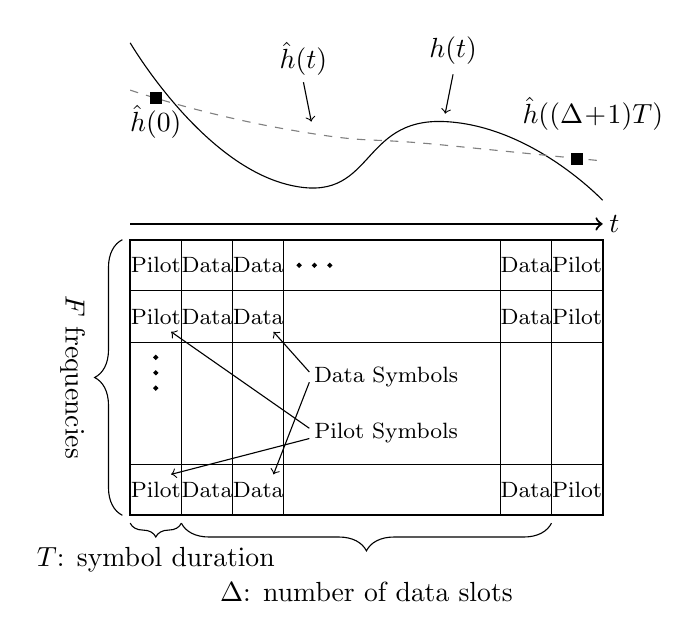
\begin{tikzpicture}[scale = 1]
  \def\x{0.65}
  \def\y{0.07}

  \draw[black, thick] (0,0) rectangle (6,3.5);

  \draw (\x,0) -- (\x,3.5);
  \draw (2*\x,0) -- (2*\x,3.5);
  \draw (3*\x,0) -- (3*\x,3.5);
  \draw (6-\x,0) -- (6-\x,3.5);
  \draw (6-2*\x,0) -- (6-2*\x,3.5);

  \draw (0, \x) -- (6, \x);
  \draw (0, 3.5-\x) -- (6, 3.5-\x);
  \draw (0, 3.5-2*\x) -- (6, 3.5-2*\x);

  \node at (\x/2, \x/2) {\footnotesize Pilot};
  \node at (\x/2, 3.5-\x/2) {\footnotesize Pilot};
  \node at (\x/2, 3.5-3*\x/2) {\footnotesize Pilot};

  \node at (3*\x/2, \x/2) {\footnotesize Data};
  \node at (3*\x/2, 3.5-\x/2) {\footnotesize Data};
  \node at (3*\x/2, 3.5-3*\x/2) {\footnotesize Data};

  \node at (5*\x/2, \x/2) {\footnotesize Data};
  \node at (5*\x/2, 3.5-\x/2) {\footnotesize Data};
  \node at (5*\x/2, 3.5-3*\x/2) {\footnotesize Data};

  \node at (6-3*\x/2, \x/2) {\footnotesize Data};
  \node at (6-3*\x/2, 3.5-\x/2) {\footnotesize Data};
  \node at (6-3*\x/2, 3.5-3*\x/2) {\footnotesize Data};

  \node at (6-\x/2, \x/2) {\footnotesize Pilot};
  \node at (6-\x/2, 3.5-\x/2) {\footnotesize Pilot};
  \node at (6-\x/2, 3.5-3*\x/2) {\footnotesize Pilot};

  \draw [->] (3.5*\x, 1.5*\x) -- (0.8*\x, 0.8*\x);
  \draw [->] (3.5*\x, 1.7*\x) -- (0.8*\x, 3.5-1.8*\x);
  \node at (5*\x, 1.6*\x) {\footnotesize Pilot Symbols};

  \draw [->] (3.5*\x, 2.6*\x) -- (2.8*\x, 0.8*\x);
  \draw [->] (3.5*\x, 2.8*\x) -- (2.8*\x, 3.5-1.8*\x);
  \node at (5*\x, 2.7*\x) {\footnotesize Data Symbols};

  \filldraw [black] (\x/2,3.5-2.3*\x) circle (0.7pt);
  \filldraw [black] (\x/2,3.5-2.6*\x) circle (0.7pt);
  \filldraw [black] (\x/2,3.5-2.9*\x) circle (0.7pt);

  \filldraw [black] (3.3*\x,3.5-\x/2) circle (0.7pt);
  \filldraw [black] (3.6*\x,3.5-\x/2) circle (0.7pt);
  \filldraw [black] (3.9*\x,3.5-\x/2) circle (0.7pt);

  \draw [decorate,decoration={brace,amplitude = 10pt}] (6-\x,-0.1) -- (\x,-0.1)
  node [black,midway,yshift=-25pt] {$\Delta$: number of data slots};
  \draw [decorate,decoration={brace,amplitude = 5pt}] (\x,-0.1) -- (0,-0.1)
  node [black,midway,yshift=-13pt] {$T$: symbol duration};


  \draw [decorate,decoration={brace,amplitude = 10pt}] (-0.1, 0) -- (-0.1,3.5)
  node [black,midway,xshift=-18pt] {\rotatebox{270}{$F$ frequencies}};

  \draw [->, thick] (0,3.7) -- (6,3.7);
  \node at (6.15, 3.7) {$t$};

  \draw plot [smooth, tension=1] coordinates { (0, 6) (2,4.2) (4,5) (6,4)};
  \draw [dashed, gray] plot [smooth, tension=1] coordinates { (0,5.4) (2,4.9) (4,4.7) (6,4.5)};

  \filldraw (\x/2-\y,5.3-\y) rectangle (\x/2+\y, 5.3+\y);
  \node at (\x/2, 5) {$\hat{\mx{h}}(0)$};
  \filldraw (6-\x/2-\y,4.52-\y) rectangle (6-\x/2+\y, 4.52+\y);
  \node at (6.2-\x/2, 5.1) {$\hat{\mx{h}}((\Delta\!+\!1)T)$};

  \draw [->] (4.1,5.6) -- (4,5.1);
  \node at (4.1, 5.9) {$\mx{h}(t)$};

  \draw [->] (2.2,5.5) -- (2.3,5);
  \node at (2.2, 5.8) {$\hat{\mx{h}}(t)$};
\end{tikzpicture}
\caption{Pilot (P) and data (D) symbols in the time-frequency domains of the system in the $(0,(\Delta+1)T)$ interval. The solid line above the
time-frequency resource grid represents the continuous time complex channel $\mx{h}(t)$, while the dashed line represents
the \ac{MMSE} channel estimate $\hat{\mx{h}}(t)$.
Notice that in each time slot of length $T$ all symbols are either pilot or
data symbols.}
\label{fig:Model}
\end{figure}

\begin{table}[t]
\caption{System Parameters}
\vspace{2mm}
\label{tab:notation}
\footnotesize
\begin{tabularx}{\columnwidth}{|X|X|}
\hline
\hline
\textbf{Notation} & \textbf{Meaning} \\
\hline
\hline
% Network layout
$K$ & Number of \ac{MU-MIMO} users \\
\hline
$N_r$ & Number of antennas at the BS \\
\hline
$F$ & Number of frequency channels used for pilot and data transmission within one slot \\
\hline
$\Delta$ & number of data slots in a data-pilot cycle \\
\hline
$\tau_p=F, \tau_d=\Delta F$ & Number of pilot/data symbols within a coherent set of subcarriers  \\
\hline
$\mx{s}\in \mathds{C}^{\tau_p \times 1}$ & Sequence of pilot symbols\\
\hline
$x$ & Data symbol \\
\hline
%$P_p, P, P_{\text{tot}}$ & Pilot power per symbol, data power per symbol, and total power budget  \\
$P_p, P$ & Pilot power per symbol, data power per symbol\\
\hline
$\mx{Y}^p(t) \in \mathds{C}^{N_r \times \tau_p}, y(t) \in \mathds{C}^{N_r}$ & Received pilot and data signal at time $t$, respectively  \\
\hline
% $\mx{N}, \mx{n}_d(t)$ & Additive white Gaussian noise at the received pilot and data signal, respectively \\
% \hline
$\alpha$ & Large scale fading between the mobile station and the base station \\
\hline
$\mx{C} \in \mathds{C}^{N_r \times N_r}$ & Stationary covariance matrix of the fast fading channel \\
\hline
$\mx{h}(t), \hat{\mx{h}}(t) \in \mathds{C}^{N_r}$ & Fast fading channel and estimated channel \\
% $\sigma_p^2 \mx{I}_{N_r}, \sigma_d^2 \mx{I}_{N_r}, \mx{C} \in \mathds{C}^{N_r \times N_r}$
% & Covariance of $\mx{N}$, $\mx{n}_d$, $\mx{h}(t)$, respectively \\
% \hline
\hline
$\bs{\varepsilon}(t) \in \mathds{C}^{N_r}, \bs{\Sigma} \in \mathds{C}^{N_r \times N_r}$
& Channel estimation error and its covariance matrix\\
\hline
%$\mx{G}, \mx{G}^\text{naive}, \mx{G}^\star$ & MU-MIMO receivers: generic, naive, and optimal, respectively. \\
$\mx{G}^\star$ & Optimal MU-MIMO receiver. \\
\hline
$f_D$ & Maximum Doppler frequency \\
\hline
$T$ & Slot duration \\
%\hline
%$\bs{\Lambda}_p$ & AWGN on the received pilot symbols at the \ac{BS} \\
\hline
\end{tabularx}
\end{table}

\subsection{Uplink Pilot Signal Model}
By extending the single antenna channel model of \cite{Savazzi:09},
each transmitting \ac{MS} uses a single time slot to send $F$ pilot symbols,
followed by $\Delta$ time slots, each of which containing $F$ data symbols according to Figure \ref{fig:Model}.
Each symbol is transmitted within a coherent time slot of duration $T$.
Thus, the total frame duration is $(1+\Delta) T$, such that each frame consists of 1 pilot
and $\Delta$ data time slots, which we will index with $i=1 \ldots \Delta$.
User-$k$ transmits each of the $F$ pilot symbols with transmit power $P_{p,k}$, and each data
symbol in slot-$i$ with transmit power $P_k(i),~k=1 \ldots K$.
To simplify notation, in the sequel we tag User-1, and will
drop index $k=1$ when referring to the tagged user.

Assuming that the coherence bandwidth accommodates at least $F$ pilot symbols,
this system allows to create $F$ orthogonal pilot sequences.
To facilitate spatial multiplexing
and \ac{CSIR} acquisition at the \ac{BS}, the \acp{MS} use orthogonal complex
sequences, such as shifted Zadoff-Chu sequences of length $\tau_p=F$, which we denote as:
\begin{align}
\mathbf{s} &\triangleq \left[s_1,...,s_{\tau_p}\right]^T \in \mathds{C}^{{\tau_p \times 1}},
\end{align}
whose elements satisfy %are scaled appropriately according to
$|s_i|^2 = 1$. %, for $i=1,..,\tau_p$ \cite{Sesia:11}.
% To enable spatial multiplexing, the length of the pilot sequences
% $\tau_p$ is chosen such that a maximum of $K$ users can be served simultaneously, implying that
% $\tau_p \geq K$ holds.
Under this assumption, the system can spatially multiplex $K\leq F$ \acp{MS}.
Focusing on the received pilot signal from the tagged user at the \ac{BS},
the received pilot signal takes the form of \cite{Fodor:21}:
\begin{align}
\mathbf{Y}^p(t)
&=
\alpha \sqrt{P_{p}}\mathbf{h}(t) \mathbf{s}^T +\mathbf{N}(t) ~~ \in \mathds{C}^{N_r \times \tau_p},
\label{eqn:received_training_seq}
\end{align}
where %we assume that
$\mathbf{h}(t) \in \mathds{C}^{N_r \times 1} \sim \mathcal{CN}(\mathbf{0},\mathbf{C})$, that is,
$\mathbf{h}(t)$ is a %circular symmetric
complex normal distributed column vector
with mean vector $\mathbf{0}$ and covariance matrix $\mx{C} \in \mathds{C}^{N_r \times N_r}$. % $\in \mathds{C}^{N_r \times N_r}$. %(of size $N_r$), %at all $t$ time instance,
Furthermore, $\alpha$ denotes
% propagation loss
large scale fading, $P_p$ denotes the pilot power of the tagged user,
and $\mathbf{N}(t)\in \mathds{C}^{N_r \times \tau_p}$
is the %spatially and temporally
\ac{AWGN} with element-wise variance $\sigma_p^2$.
It will be convenient to introduce $\mathbf{\tilde Y}^p(t)$ by stacking the columns of  $\mathbf{Y}^p(t)$ as:
\begin{align}
\mathbf{\tilde Y}^p(t)=\textbf{vec}\big(\mathbf{Y}^p(t)\big)=\alpha\sqrt{P_p} \mathbf{S} \mathbf{h}(t) +\mathbf{\tilde N}(t) ~\in \mathds{C}^{\tau_p N_r \times 1},
\label{eqn:received_training_seq2}
\end{align}
where $\textbf{vec}$ is the column stacking vector operator,
$\mathbf{\tilde Y}^p(t)$, $\mathbf{\tilde N}(t) \in \mathds{C}^{\tau_p N_r \times 1}$
and
$\mathbf{S} \triangleq \mathbf{s}\otimes \mathbf{I}_{N_r} \in \mathds{C}^{\tau_p N_r \times N_r}$
is such that $\mathbf{S}^H\mathbf{S}=\tau_p\mathbf{I}_{N_r}$,
where $\mathbf{I}_{N_r}$ is the identity matrix of size $N_r$.
\vspace{-2mm}
\subsection{Channel Model}
\vspace{-1mm}
% Consider a single block of $\Delta$ data symbols sent at time instances $iT$ for $i = 1\ldots \Delta$
% and a pilot symbol sent at time $0$ and subsequently at $(\Delta+1)T$.
In \eqref{eqn:received_training_seq},
the channel $\mx{h}(t)$ evolves continuously according to a multivariate complex stochastic process
with stationary covariance matrix $\mx{C}$.
That is, for symbol duration $T$, the channel ($\mx{h}(t)$) evolves according to the following \ac{AR} process:
\begin{align}
\label{eq:AR1}
\mx{h}(t+T) &= \mx{A} \mx{h}(t) + \bs{\vartheta}(t),
\end{align}
where the transition matrix of the \ac{AR} process is denoted by $\mx{A}$.
This \ac{AR} model has been commonly used to approximate Rayleigh fading channels in e.g. \cite{Baddour05}.
Equation \eqref{eq:AR1} implies that the autocorrelation function of the channel process is:
\begin{align}
\mathds{E}\left(\mx{h}(t)\mx{h}^H(t+iT)\right) &= \mx{C}\left(\mx{A}^H\right)^i, \quad \forall i.
\end{align}
%satisfies the following equation:
Consequently, the autocorrelation function of
the fast fading channel ($\mx{h}(t)$) is modelled as:
\begin{align}
\label{eq:autocorr}
\mx{R}(i) \triangleq
\mathds{E}\left(\mx{h}(t)\mx{h}^H(t+iT)\right) &= \mx{C} e^{\mx{Q}^H i T },
\end{align}
where matrix $\mx{Q}$ describes the correlation decay, such that:
\begin{align}
e^{\mx{Q}T} = \mx{A}.
\end{align}

Similarly, for user $k$,
\begin{align}
\label{eq:autocorrk}
\mx{R}_k(i) \triangleq
\mathds{E}\left(\mx{h}_k(t)\mx{h}_k^H(t+iT)\right) &= \mx{C}_k e^{\mx{Q}_k^H i T },
\end{align}

%We denote by $R(i) \triangleq cJ_0(2 \pi f_D i T)$ the correlation between the $i$-th element of
%the channel vectors that are $i \cdot T$ apart from each other in time.
% For the pilot channels we
In each pilot slot,
the \ac{BS} utilizes \ac{MMSE} channel estimation to obtain the channel estimate of each user, as it will be detailed in Section \ref{Sec:ChannelE}.
Without loss of generality, to simplify the notation, hereafter we assume that the time unit is $T$ and $iT=i$.

\begin{comment}
\begin{align}
\label{eq:LS}
\hat{\mx{h}}(t) &= \mx{h}(t) + \boldsymbol{\varepsilon}(t), \\
\boldsymbol{\varepsilon}(t) & \sim
%\mathcal{CN}\left(0,\frac{\boldsymbol{\Lambda}_p}{\alpha^2 F P_p} \right) \triangleq
\mathcal{CN}\left(0,\mx{\Sigma}\right)
\text{~with~} \mx{\Sigma} = \frac{\boldsymbol{\Lambda}_p}{\alpha^2 F P_p}
\end{align}
where $\mathcal{CN}\left(0,\mx{\Sigma}\right)$ is the $N_r$ dimensional complex normal distribution with mean $0$ and covariance matrix $\mx{\Sigma}$,  $\boldsymbol{\Lambda}_p$ is the covariance matrix of the \ac{AWGN} on the pilot symbols at the receiver
and $\alpha$ is the path loss between the \ac{MS} and the \ac{BS} \cite{Fodor:21}, which are assumed to be identical for all $F$ frequencies.
\end{comment}


\subsection{Data Signal Model}
When spatially multiplexing $K$ \ac{MU-MIMO} users,
the received data signal at the \ac{BS} at time $t$ is \cite{Fodor:21}:

\begin{align}
\mathbf{y}(t)
&=
\underbrace{\mathbf{\alpha} \mathbf{h}(t) \sqrt{P} x(t)}_{\text{tagged user}}
+ \underbrace{\sum_{k=2}^K \mathbf{\alpha}_{k} \mathbf{h}_k(t) \sqrt{P_{k}} x_{k}(t)}_{\text{co-scheduled MU-MIMO users}}
% \underbrace{\sum_{i \neq 1}^L \sum_{k=1}^K \mathbf{g}_{1,i,k} \sqrt{P_{i,k}} x_{i,k}}_{\text{Other cells}}
+\mathbf{n}_d(t),
%~~\in \mathds{C}^{N_r \times 1},
\label{eq:mumimo2}
\end{align}
\noindent where $\mathbf{y}(t)\in \mathds{C}^{N_r \times 1}$;
% and $\mathbf{\alpha}_{k} \mathbf{h}_k(t) \in \mathds{C}^{N_r \times 1}$
% denotes the channel vector,
and $x_k(t)$ denotes the transmitted data symbol of User-$k$
at time $t$ with transmit power $P_k$.
Furthermore, $\mathbf{n}_d(t)~\sim \mathcal{CN}\left(\mx{0},\sigma_d^2 \mathbf{I}_{N_r}\right)$
is the \ac{AWGN} at the receiver.
\vspace{-2mm}
\section{Channel Estimation}
\label{Sec:ChannelE}
In this section, we are interested in calculating the \ac{MMSE} estimation of the
channel in each slot $i$, based on received pilot signals, as a function of the frame
size corresponding to pilot spacing (see $\Delta$ in Figure \ref{fig:Model}).
Note that estimating the channel at the receiver can be based on
multiple received pilot signals both before and after the actual data slot $i$.
While using pilot signals that are received before data slot $i$ requires to
store the samples of the received pilot, using pilot signals that arrive after
data slot $i$ necessarily induces some delay in estimating the transmitted data symbol.
In the numerical section, we will refer to specific channel estimation strategies
as, for example, "1 before, 1 after" or "2 before, 1 after" depending on the number
of utilized pilot signals received prior to or following data slot $i$
for \ac{CSIR} acquisition.
In the sequel we use the specific case of "2 before, 1 after" to illustrate the
operation of the \ac{MMSE} channel estimation scheme,
that is when the receiver uses the pilot signals
$\mathbf{\tilde Y}^p(-\Delta-1)$, $\mathbf{\tilde Y}^p(0)$, and $\mathbf{\tilde Y}^p(\Delta+1)$
for \ac{CSIR} acquisition.
We are also interested in determining the distribution of the
resulting channel estimation error, whose covariance matrix, denoted by
$\mx{Z}(\Delta,i)$, will play an important role in subsequently determining
the deterministic equivalent of the \ac{SINR}.
\vspace{-2mm}
\subsection{\ac{MMSE} Channel Estimation and Channel Estimation Error}
As illustrated in Figure \ref{fig:Model},
in each data slot $i$, the \ac{BS} utilizes the \ac{MMSE} estimates of the channel
obtained in the neighboring pilot slots, for example at $(-\Delta-1)$, $0$ and $(\Delta+1)$, %according to \eqref{eqn:received_training_seq2}.
using the respective received pilot signals according to \eqref{eqn:received_training_seq2}, that is
$\mathbf{\tilde Y}^p\big((-\Delta-1)\big)$, $\mathbf{\tilde Y}^p(0)$ and $\mathbf{\tilde Y}^p\big((\Delta+1)\big)$, using the following lemma.

\begin{lem}
\label{lem:mmsechannel}	
The \textup{MMSE} channel estimator approximates the autoregressive fast fading channel in time slot $i$
based on the received pilots at $(-\Delta-1)$, $0$ and $(\Delta+1)$ as
\begin{align}
\label{eq:hmmse}
&\mathbf{\hat h}_{\textup{MMSE}}(\Delta,i)=
\mx{H^\star}(\Delta,i) \mathbf{\hat Y}^p(\Delta),
\end{align}
where
\begin{align*}
\mx{H^\star}(\Delta, i) = \frac{1}{\alpha \sqrt{P_p} \tau_p} \mx{E}(\Delta,i). \big(\mx{M}(\Delta)+\mx{\Sigma}_3\big)^{-1}.(\mx{s}^H\otimes \mx{I}_{3N_r}),
\end{align*}

$\mathbf{\hat Y}^p(\Delta) \triangleq \begin{bmatrix}
\mathbf{\tilde Y}^p((-\Delta-1)) \\
\mathbf{\tilde Y}^p(0) \\
\mathbf{\tilde Y}^p((\Delta+1))
\end{bmatrix}$~~and~~$\mx{\Sigma}_3\triangleq \frac{\sigma_p^2}{\alpha^2P_p \tau_p} \mx{I}_{3N_r}$,
\begin{align}
\label{eq:E}
\mx{E}(\Delta,i) &\triangleq
\begin{bmatrix}
\mx{R}(\Delta \!+\! 1 \!+\! i) & \mx{R}(i) &
\mx{R}(\Delta \!+\! 1 \!-\! i)
\end{bmatrix},
\\
\label{eq:M}
\mx{M}(\Delta) &\triangleq
\begin{bmatrix}
\mx{C} & \mx{R}(\Delta \!+\! 1) & \mx{R}(2\Delta \!+\! 2)  \\
\mx{R}^H(\Delta \!+\! 1) & \mx{C} & \mx{R}(\Delta \!+\! 1) \\
\mx{R}^H(2\Delta \!+\! 2) & \mx{R}^H(\Delta \!+\! 1) & \mx{C}\\
\end{bmatrix}.
\end{align}

\end{lem}

\begin{proof}
The \ac{MMSE} channel estimator aims at minimizing the \ac{MSE} between the channel estimate
$\mathbf{\hat h}_{\textrm{MMSE}}(\Delta, i) = \mathbf{H}^\star(\Delta, i) \mathbf{\hat Y}^p(\Delta)$ and the channel $\mathbf{h}(i)$, that is
\begin{align}
\mathbf{H^\star}(\Delta, i)= \text{arg} \min_{\mathbf{H}} \mathds{E}_{\mathbf{h},\mathbf{n}}\{ ||\mathbf{H} \mathbf{\hat Y}^p(\Delta) - \mathbf{h}(i)||^2 \}.
\end{align}
The solution of this quadratic optimization problem is
$\mathbf{H^\star}(\Delta, i)= \mx{a}(\Delta, i)^H \mx{F}^{-1}(\Delta)$
with
\begin{align}
\label{eq:Fandb}
\mx{F}(\Delta) &\triangleq \mathds{E}_{\mathbf{h},\mathbf{n}}\left(\mx{\hat Y}^p(\Delta) \left(\mx{\hat Y}^p(\Delta)\right)^H\right), \\
\mx{a}(\Delta, i) &\triangleq \mathds{E}_{\mathbf{h},\mathbf{n}}\left( \mx{\hat Y}^p(\Delta) \mx{h}^{H}(i)\right).
\end{align}
Let
\begin{align}
\mx{\bar h}(\Delta) \triangleq \begin{bmatrix}
\mx{h}((-\Delta-1)) \\
\mx{h}(0) \\
\mx{h}((\Delta+1))
\end{bmatrix} \nonumber
\end{align}
and
\begin{align}
\mx{\tilde{\bar{N}}}(\Delta) \triangleq \begin{bmatrix}
\mx{\tilde{N}}((-\Delta-1)) \\
\mx{\tilde{N}}(0) \\
\mx{\tilde{N}}((\Delta+1))
\end{bmatrix}.
\end{align}
Using $\mx{\bar h}(\Delta)$, we have
\begin{align}
\begin{bmatrix}
\mx{S}\mx{h}((-\Delta-1)) \\
\mx{S}\mx{h}(0) \\
\mx{S}\mx{h}((\Delta+1))
\end{bmatrix}=
\begin{bmatrix}
\mx{S}  & \mx{0} & \mx{0} \\
\mx{0} & \mx{S}  & \mx{0} \\
\mx{0} & \mx{0} & \mx{S}
\end{bmatrix}\mx{\bar h}(\Delta)
\nonumber \\
~~~~~~~~= (\mx{I}_3\otimes\mx{S}) \mx{\bar h}(\Delta)=  (\mx{s}\otimes \mx{I}_{3N_r}) \mx{\bar h}(\Delta).
\end{align}
Since $\mx{\bar h}(\Delta)$ and $\mx{\tilde{\bar{N}}}(\Delta)$ are independent and
\begin{align}
\mathds{E}_{\mathbf{h},\mathbf{n}}(\mx{\bar h}(\Delta)\mx{\bar h}^H(\Delta))&=\mx{M}(\Delta),\\
\mathds{E}_{\mathbf{h},\mathbf{n}}(\mx{h}(i)\mx{\bar h}^H(\Delta))&=\mx{E}(\Delta,i).
\end{align}
Therefore, for $\mx{F}(\Delta)$ and $\mx{a}(\Delta,i)$, we have
\begin{align*}
\mx{F}(\Delta) &=
%\mathds{E}_{\mathbf{h},\mathbf{n}}\left(\mx{\tilde{\bar{Y}}}^p\mbox{$\mx{\tilde{\bar{Y}}}^p$}^H\right)\\&=
\mathds{E}_{\mathbf{h},\mathbf{n}}
\left(\left(\alpha\sqrt{P_p} (\mx{I}_3\otimes\mx{S}) \mx{\bar{h}}(\Delta) +\mx{\tilde{\bar{N}}}(\Delta)\right)\right.\nonumber \\
&~~~~~~~~~~~~\cdot \left.\left(\alpha\sqrt{P_p} (\mx{I}_3\otimes\mx{S}) \mx{\bar{h}}(\Delta) +\mx{\tilde{\bar{N}}}(\Delta)\right)^H\right)\\
&=\alpha^2P_p(\mx{I}_3\otimes\mx{S})\mx{M}(\Delta)\left(\mx{I}_3\otimes\mx{S}^H\right)+ \sigma_p^2 \mathbf{I}_{3N_r\tau_p},\\
\mx{a}(\Delta, i) &= \mathds{E}_{\mathbf{h},\mathbf{n}}\left( \mx{\hat Y}(\Delta) \mx{h}^{H}(i)\right) \\
&=\mathds{E}_{\mathbf{h},\mathbf{n}}
\left(\left(\alpha\sqrt{P_p} (\mx{I}_3\otimes\mx{S}) \mx{\bar{h}}(\Delta) +\mx{\tilde{\bar{N}}}(\Delta)\right)
\mx{h}^{H}(i)\right)\\
&= \alpha\sqrt{P_p} ~(\mx{I}_3\otimes\mx{S})~\mx{E}(\Delta,i)^T,
\end{align*}
which yields Lemma \ref{lem:mmsechannel}.
\end{proof}

The \ac{MMSE} estimate of the channel is then expressed as:
\begin{align}
\nonumber
&\mathbf{\hat h}_{\textrm{MMSE}}(\Delta, i)=\mathbf{H^\star}(\Delta, i) \mathbf{\hat Y}^p(\Delta) ~~~~ \\
&~~~~=\mathbf{H^\star}(\Delta, i)
\left(\alpha\sqrt{P_p} (\mx{I}_3\otimes\mx{S}) \mx{\bar{h}}(\Delta) +\mx{\tilde{\bar{N}}}(\Delta)\right)
\nonumber
\\
&~~~~=
\frac{1}{\alpha\sqrt{P_p} \tau_p}
\mx{E}(\Delta, i) \left(   \mx{M}(\Delta) + \mx{\Sigma}_{3} \right)^{-1}
\nonumber
\\&~~~~~~~~~~.
\left(\alpha\sqrt{P_p} \tau_p \mx{\bar{h}}(\Delta) + \left(\mx{I}_3 \otimes \mx{S}^H\right) \mx{\tilde{\bar{N}}}(\Delta)\right).
\label{eq:MMSEt}
\end{align}

Next, we are interested in deriving the distribution of the estimated channel and
the channel estimation error, since these will be important for understanding the
impact of pilot spacing on the achievable \ac{SINR} and spectral efficiency of
the \ac{MU-MIMO} system. To this end, the following two corollaries of
Lemma \ref{lem:mmsechannel} and \eqref{eq:MMSEt} will be important in the sequel.
\begin{cor}
\label{cor:rmmse}	
The estimated channel $\mathbf{\hat h}_{\textup{MMSE}}(\Delta, i)$ is a circular symmetric complex normal distributed vector
$\mathbf{\hat h}_{\textup{MMSE}}(\Delta, i) \sim %\mathcal{CN}(\mathbf{0},\mathbf{R}_{\textup{MMSE}}(\Delta, i))$,
\mathcal{CN}\Big(\mathbf{0},\mathbf{\hat \Phi}_{\textup{MMSE}}(\Delta, i)\Big)$,
with
\begin{align}
\label{eq:rmmse}
\mathbf{\hat \Phi}_{\textup{MMSE}}(\Delta, i) \triangleq
& \mathds{E}_{\mathbf{h},\mathbf{n}} \{\mathbf{\hat h}_{\textup{MMSE}}(\Delta, i) \mathbf{\hat h}_{\textup{MMSE}}^H(\Delta, i)\}
 \nonumber \\
=& \mx{E}(\Delta, i) \big(\mx{M}(\Delta)+\mx{\Sigma}_3\big)^{-1} \mx{E}(\Delta, i)^H.
\end{align}

\end{cor}

\begin{proof}
Equation \eqref{eq:rmmse} follows directly from \eqref{eq:MMSEt}.	
\end{proof}

An immediate consequence of Corollary \ref{cor:rmmse}
is the following corollary regarding the covariance of the channel estimation
error, as a function of pilot spacing.
\begin{cor}
\label{Cor:ChEstError}
The channel estimation error in slot $i$, $\mx{\hat{h}}_{\textup{MMSE}}(\Delta, i)-\mx{h}(\Delta, i)$,
is complex normal distributed with zero mean vector and
covariance matrix given by:
\begin{align}
\label{eq:Z}
\mx{Z}(\Delta, i) \triangleq  \mx{C} -
\mx{E}(\Delta, i) \big(\mx{M}(\Delta)+\mx{\Sigma}_3\big)^{-1}
\mx{E}(\Delta, i)^H.
\end{align}
\end{cor}

In the following section we will calculate the \ac{SINR} of the received data symbols.
For simplicity of notation, we use $\mx{\hat h}_{\textup{MMSE}}(\Delta, i)=\mx{\hat h}(\Delta, i)$, and  introduce
$$\mx{b}(\Delta, i) \triangleq \alpha\sqrt{P(i)}\mx{\hat{h}}(\Delta, i)$$
with covariance matrix
\begin{align}
\label{eq:Phi}
\bs{\Phi}(\Delta, i) & \triangleq
\mathds{E}\left( \mx{b}(\Delta, i)\mx{b}^H(\Delta, i) \right)  \nonumber \\
&=\mathds{E}\left( \Big(\alpha\sqrt{P(i)} \mx{\hat{h}}(\Delta, i) \Big)\Big(\alpha\sqrt{P(i)} \mx{\hat{h}}(\Delta, i) \Big)^H  \right)  \nonumber \\
&=\alpha^2P(i)(\mx{C}-\mx{Z}(\Delta, i)).
\end{align}
% \dg{For consistency, shouldn't we use $P_i$ instead of $P(i)$?}
\subsection{Summary}

This section derived the \ac{MMSE} channel estimator (Lemma \ref{lem:mmsechannel})
that uses the received pilot signals
both before and after a given data slot $i$ and depends on the frame size $\Delta$ (pilot spacing).
As important corollaries of the channel estimation scheme, we established the distribution
of both the estimated channel (Corollary \ref{cor:rmmse})
and the associated channel estimation error in each data
slot $i$ (Corollary \ref{Cor:ChEstError}), as functions of both the employed pilot spacing and pilot power. These
results serve as a starting point for deriving the achievable \ac{SINR} and spectral
efficiency.

\section{\ac{SINR} Calculation}
\label{Sec:SINR}

\subsection{Instantaneous \ac{SINR}}
We start with recalling an important lemma from \cite{Fodor:22}, which calculates the instantaneous \ac{SINR}
in an \ac{AR} fast fading environment
when the \ac{BS} uses the \ac{MMSE} estimation of the fading channel, and employs the optimal linear
receiver:
\begin{align}
\label{eq:Gstar2}
\mx{G}^\star(\Delta, i) &=
% \textup{arg} \min_{\mx{G}} \textup{MSE}\left(\mx{G},\mx{\hat H}(t), \mx{\hat H}(t-1)\right)
\mx{b}^H(\Delta,i) \mx{J}^{-1}(\Delta,i),
\end{align}
where $\mx{J}(\Delta, i) \in \mathds{C}^{N_r \times N_r}$
is defined as
\begin{align}
%\label{eq:A3}
\nonumber
\mx{J}(\Delta, i)
&\triangleq
\sum_{k=1}^K  \mx{b}_k(\Delta, i) \mx{b}_k^H(\Delta, i) + \bs{\beta}(\Delta, i),
\end{align}
where
\begin{align}
\label{eq:beta}
\bs{\beta}(\Delta, i) \triangleq \sum_{k=1}^K \alpha_k^2 P_k  \mx{Z}_k(\Delta, i) + \sigma^2_d \mx{I}_{N_r}.
\end{align}
%and $\mx{I}$ is the identity matrix of size $N_r$.

When using the above receiver, which minimizes the \ac{MSE} of the received data symbols in the
presence of channel estimation errors, the following result from \cite{Fodor:22} will be useful in the sequel:
\begin{lem}[See \cite{Fodor:22}, Lemma 3]
Assume that
the receiver employs \textup{\ac{MMSE}} symbol estimation,
that is it employs the optimal linear receiver $\mx{G}^\star(\Delta, i)$ given in \eqref{eq:Gstar2}. %and the instantaneous channel estimates,
Then the instantaneous \textup{\ac{SINR}} of the estimated data symbols of the tagged user,
$\gamma(\Delta, i)$ %\Big(\mathbf{G}^\star, \hat{\mathbf{H}}(t),\hat{\mathbf{H}}(t-1)\Big)$
is given as:
% the instantaneous \textup{\ac{SINR}} of the data symbols, can be expressed as:
%
\begin{equation}
\label{eq:lemma2Eq}
\gamma(\Delta, i) %\Big(\mathbf{G}^\star(t), \hat{\mathbf{H}}(t),\hat{\mathbf{H}}(t-1)\Big)
=
\mx{b}^H(\Delta, i) \mathbf{\bar{J}}^{-1}(\Delta, i) \mx{b}(\Delta, i),
\end{equation}
where
\vspace{-1mm}
\begin{equation}
\mathbf{\bar{J}}(\Delta, i) \triangleq \mathbf{J}(\Delta, i)- \mx{b}(\Delta, i)\mx{b}^H(\Delta, i).
\end{equation}
\end{lem}
\begin{comment}
Using the \ac{MMSE} estimate $\bar{\mx{h}}(i) = \mx{E}(i) \mx{\hat{\bar{h}}}(\Delta)$ of the channel $\mx{h}(i)$,
we can calculate the \ac{SINR} of the estimated data symbol sent at time $i$ when the \ac{BS} employs an optimal linear receiver as provided in \cite{Fodor:22}.
Lemma 2 in \cite{Fodor:22} shows that when $K$ \acp{MS} enumerated $k = 1 \ldots K$ transmit data signals
through channels $\mx{h}_k$ with \ac{MMSE} estimates
$\bar{\mx{h}}_k$, estimation error covariance $\mx{Z}_k$, path losses $\alpha_k$,
and employing transmit powers $P_k$, the \ac{SINR} of the estimated data symbol of user $k$, $\hat x = \mx{G}\mx{y}$:

\begin{align}
    \gamma_k = \alpha_k^2 P_k \bar{\mx{h}}_k^H \left( \sum_{l \neq k}^K \alpha_l^2 P_l \bar{\mx{h}}_l\bar{\mx{h}}_l^H
    + \sum_{l = 1}^K \alpha_l^2 P_l \mx{Z}_l + \sigma_d^2 \mx{I} \right)^{-1}\bar{\mx{h}}_k,
\end{align}

where $\sigma_d^2$ is the variance of the \ac{AWGN} on the data signal.
Applying this formula on the previous section, where the data symbol of User-$k$, in data time slot $i$ is transmitted through the channel $\mx{h}_k(iT)$,
with \ac{MMSE} estimate $\bar{\mx{h}}_k(iT) = \mx{E}_k(i) \bs{\zeta}_k(\Delta)$ and channel covariance matrix $\mx{Z}(i)$
the \ac{SINR} of the estimated data symbol sent by User-$k$ is given by
\end{comment}
For the \ac{AR} fading case considered in this paper,
based on the definitions of $\mx{b}(\Delta, i)$, $\mx{J}(\Delta, i)$ and $\mx{\bar{J}}(\Delta, i)$,
the instantaneous \ac{SINR} of the tagged user is then expressed as:
\begin{align}
\gamma(i) &  =  \mx{b}^H(\Delta, i) \mathbf{\bar{J}}^{-1}(\Delta, i) \mx{b}(\Delta, i)
  \nonumber\\
 &=
\textup{tr}\left( \mx{b}(\Delta, i)\mx{b}^H(\Delta, i) \mathbf{\bar{J}}^{-1}(\Delta, i) \right).
\end{align}

\subsection{Slot-by-Slot Deterministic Equivalent of the \ac{SINR} as a Function of Pilot Spacing $\Delta$}
We can now prove the following important proposition that gives the asymptotic deterministic equivalent
of the instantaneous \ac{SINR} in data slot $i$, $\bar{\gamma}(\Delta, i)$, when the number of antennas $N_r$ approaches infinity.
This asymptotic equivalent \ac{SINR} gives a good approximation of averaging the instantaneous \ac{SINR} of the tagged user \cite{Wagner:2012, Hoydis:13, Fodor:22}.

\begin{prop}
\label{Prop:SINR}
% According to this theorem, for User-$1$ the \ac{SINR} is given by
The asymptotic deterministic equivalent \ac{SINR} of the tagged user in data slot $i$ can be calculated as:
\begin{align}
\label{eq:hoydis1}
\bar{\gamma}(\Delta, i) &= \textup{tr}\Big( \bs{\Phi}(\Delta, i)\mx{T}(\Delta, i)  \Big),
\end{align}
where $\mx{T}(\Delta, i)$ is defined as: %given by
\begin{align}
\label{eq:hoydis2}
\mx{T}(\Delta, i) \triangleq \left( \sum_{m = 2}^{K} \frac{\bs{\Phi}_m(\Delta, i)}{1 + \delta_m(\Delta, i)} + \bs{\beta}(\Delta, i) \right)^{-1},
\end{align}
and $\delta_m(\Delta, i)$ are the solutions of the following system of $K$ equations
\begin{align}
\label{eq:hoydis3}
\delta_m(\Delta, i) &= \textup{tr}\left(\bs{\Phi}_m(\Delta, i)
\left( \sum_{l = 2}^{K} \frac{\bs{\Phi}_l(\Delta, i)}{1 + \delta_l(\Delta, i)} + \bs{\beta}(\Delta, i)  \right)^{-1} \right)
\end{align}
for $\forall m = 1, \ldots, K$.
\end{prop}
The above system of $K$ equations gives the deterministic equivalent of the \ac{SINR} of the tagged user,
and a different set of $K$ equations must be used for each user.
\begin{proof}
The $\mx{b}_k(\Delta, i)$ vectors are independent for $k = 1 \ldots K$,
and the covariance matrix of $\mx{b}_k(\Delta, i)$ is $\bs{\Phi}_k(\Delta, i)$
(c.f. \eqref{eq:Phi}).
We can then express the expected value of the \ac{SINR} of the tagged user as follows:
\begin{align}
\label{eq:gammaB}
& \bar{\gamma}(\Delta, i) \triangleq \mathds{E}\Big(\gamma(\Delta, i)\Big)   \\
&= \mathds{E}\left( \textup{tr}\left( \bs{\Phi}(\Delta, i)  \left( \sum_{l = 2}^K  \mx{b}_l(\Delta, i) \mx{b}_l^H(\Delta, i)  +\bs{\beta}(\Delta, i) \right)^{\!\!-1}  \right) \right).
\nonumber
\end{align}
%We proceed
The proposition is established
by invoking Theorem \ref{thm:upperbound} in \cite{Wagner:2012}, which is applicable in multiuser systems and
% Theorem \ref{thm:upperbound} in \cite{Wagner:2012}
gives the value of the deterministic equivalent of $\bar{\gamma}(\Delta, i)$
implicitly using a system of $K$ equations and noticing that
$\bar{\gamma}(\Delta, i) = \delta_1(\Delta, i)$, since $\delta_1(\Delta, i)=\textup{tr}\big( \bs{\Phi}(\Delta, i) \mx{T}(\Delta, i)\big)$ according to \eqref{eq:hoydis3}.
\end{proof}

\subsection{Summary}
This section established the instantaneous slot-by-slot \ac{SINR} of a tagged user ($\bar \gamma(i)$) of a \ac{MU-MIMO} system operating over %continuous time
a fast fading channels modelled as \ac{AR} processes,
by applying our previous result obtained for discrete-time \ac{AR} channels
reported in \cite{Fodor:21}.
Next, we invoked Theorem \ref{thm:upperbound} in \cite{Wagner:2012}, to establish the deterministic
equivalent \ac{SINR} for each slot, as a function of the frame size (pilot spacing) $\Delta$, see Proposition \ref{Prop:SINR}.
These results serve as a basis for formulating the pilot spacing optimization problem over the frame size and pilot power as optimization variables.

\section{Pilot Spacing and Power Control}
\label{Sec:PilotSpacing}
In this section, we study the impact of pilot spacing and power control on the achievable \ac{SINR}
and the \ac{SE} of all users in the system.
The asymptotic \ac{SE} of the $i$-th data symbol of user $k$ is
\begin{align}
\label{eq:SE}
\text{SE}_k(\Delta, i) \triangleq \log\Big(1 + \bar{\gamma}_k(\Delta, i)\Big),
\end{align}
where $\bar{\gamma}_k(\Delta, i)$ denotes the average \ac{SINR} of  user $k$ when sending the $i$-th data symbol, and when $\Delta$ data symbols are sent between every pair of pilot symbols.
Consequently, the %information rate
average \ac{SE}
of  user $k$ over the $(\Delta+1)$ slot long frame is
\begin{align}
\frac{\sum_{i=1}^{\Delta}\text{SE}_k(\Delta, i)}{\Delta + 1},
\end{align}
which can be optimized over $\Delta$.
More importantly, %the sum information rate
the aggregate average \ac{SE}
of the \ac{MU-MIMO} system for the $K$ users can be expressed as:
\begin{align}
\text{SE}(\Delta) = \frac{\sum_{k=1}^K \sum_{i=1}^{\Delta}\text{SE}_k(\Delta,i)}{\Delta + 1}.
\label{eq:multiopt}
\end{align}


\subsection{An Upper Bound of the Deterministic Equivalent \ac{SINR} and the \ac{SE}}

Let us assume that $\mx{Q}_k=q_k \mx{I}_{N_r}$, that is the
channel vector $\mx{h}_k(t)$ consists of independent \ac{AR} processes in the spatial domain, implying that:
\begin{align}
\label{eq:r1}
\mx{R}_k(i) \triangleq
\mathds{E}\left(\mx{h}_k(t)\mx{h}_k^H(t+i)\right) &= \mx{C}_k e^{q_k^* i},
\end{align}
where $q_k$ is a scalar, $q_k^*$ denotes complex conjugation, and let $\bar{q}_k\triangleq Re(q_k)<0$.

Note that the exponential approximation of the autocorrelation function of the fast fading process expressed
in \eqref{eq:r1} is related to the Doppler frequency of Rayleigh fading through:
\begin{align}
\label{eq:RayleighApprox}
\underbrace{\mx{C}J_0(2 \pi f_D i)}_{\text{True autocorrelation of Rayleigh fading}} &\approx \mx{R}(i),
\end{align}
where $J_0(.)$ is the zeroth order Bessel function \cite{Wang:03}.
Based on the exponential approximation of this Rayleigh fading process in \eqref{eq:r1}, the Doppler frequency of the approximate model is obtained from $2 \pi f_D i = Re(q_k^* i)$, i.e. $f_D = 2 \pi/\bar{q}_k$.

To optimize \eqref{eq:multiopt}, we first find an upper bound of $\text{SE}_k(\Delta,i)$
via an upper bound of $\bar{\gamma}_k(\Delta, i)$.
To simplify the notation, the following discussion refers to the tagged user, and later we utilize that the same relations hold for all users.
We introduce the following upper bound of $\bar{\gamma}(\Delta, i)$:
\begin{align}
\label{eq:upper}
\bar{\gamma}^{(u)}(\Delta, i) \!&\triangleq \textup{tr}\!\left(\! \bs{\Phi}^{(u)}(\Delta, i)  \left(\sum_{l = 1}^K \!\alpha_l^2 P_l \mx{Z}^{(u)}_l(\Delta, i) \!+\! \sigma_d^2 \mx{I_{N_r}}\right)^{\!\!\!-1}  \!\right)\!,
\end{align}
where $\mx{Z}^{(u)}(\Delta, i)$ and $\bs{\Phi}^{(u)}(\Delta, i)$ are given by
\begin{align}
\label{eq:zu}
\mx{Z}^{(u)}(\Delta, i) &\triangleq \mx{C} - \rho(\Delta, i) \mx{C} \left(\eta  \mx{C} + \bs{\Sigma} \right)^{-1} \mx{C},  \\
\label{eq:phiu}
\bs{\Phi}^{(u)}(\Delta, i) &\triangleq \alpha^2 P \rho(\Delta, i) \mx{C} \left( \eta \mx{C} + \bs{\Sigma} \right)^{-1} \mx{C},
\end{align}
with $\eta$ being a constant, $\mx{\Sigma}\triangleq \frac{\sigma_p^2}{\alpha^2P_p \tau_p} \mx{I}_{N_r}$ and
\begin{align}
\label{eq:rho}
%\mx{\Sigma} &\triangleq \frac{\sigma_p^2}{\alpha^2P_p %\tau_p} \mx{I}_{N_r} \\
\rho(\Delta, i) &\triangleq e^{2\bar{q} (\Delta + 1 + i)} + e^{2\bar{q}  i} + e^{2\bar{q} (\Delta + 1 - i)}.
\end{align}

\begin{thm}
\label{thm:upperbound}
If $\bar{q}<0$ and
\begin{align}
\label{eq:etacond}
0<\eta<\frac{1}{2}\left(2+a^2-a\sqrt{8+a^2}\right),
\end{align}
with $a\triangleq e^{2\bar{q}}$
then  $\bar{\gamma}(\Delta, i)\leq \bar{\gamma}^{(u)}(\Delta, i)$.
\end{thm}
%\overset{(a)}{=}
\begin{proof}
We prove the theorem based on the following inequalities
\begin{align}
\bar{\gamma}(\Delta, i)
&\overset{(a)}{\leq}
\textup{tr}\left( \bs{\Phi}(\Delta, i) \bs{\beta}(\Delta, i)^{-1} \right) \nonumber \\
&\overset{(b)}{\leq}
   \textup{tr}\left( \bs{\Phi}^{(u)}(\Delta, i) \bs{\beta}(\Delta, i)^{-1} \right)
\overset{(c)}{\leq}
   \bar{\gamma}^{(u)}(\Delta, i),  \label{eq:gammabound}
\end{align}
which are proved in consecutive lemmas.
\end{proof}

%The following properties of positive semi-definite matrices are essential to prove the theorem.
\begin{lem}
\label{lem:AB}
Let $\mx{A}$, $\mx{B}$ and $\mx{C}$ be positive definite matrices and $\mx{D}$ be any matrix, such that $\mx{A} \preceq \mx{B}$ (i.e. $\mx{B}-\mx{A}$ is a positive semidefinite matrix), then
\begin{align}
\label{eq:ABinv}
\mx{A}^{-1} &\succeq \mx{B}^{-1},
\\
\label{eq:AB3}
\textup{tr}\left( \mx{D}^H \mx{A} \mx{D} \right) &\leq \textup{tr}\left(\mx{D}^H \mx{B} \mx{D} \right) \\
\label{eq:AB1}
\textup{tr}\left( \mx{A} \mx{C} \right) &\leq \textup{tr}\left(\mx{B} \mx{C} \right)
\\
\label{eq:AB2}
\textup{tr}\left( \mx{C} \mx{A}^{-1} \right) &\geq \textup{tr}\left( \mx{C} \mx{B}^{-1} \right).
\end{align}
\end{lem}
\begin{proof}
$\mx{A}^{-1} \succeq \mx{B}^{-1}$ is given in \cite[p. 495, Corollary 7.7.4(a)]{Horn2013}.
\eqref{eq:AB3} follows from the fact that $\mx{D}^H (\mx{B}-\mx{A}) \mx{D}$ is a positive semidefinite matrix since $\mx{B}-\mx{A}$ is a positive semidefinite matrix and
for any $\mx{x}$
\begin{align}
\mx{x}^H \mx{D}^H (\mx{B}-\mx{A}) \mx{D} \mx{x} = \mx{y}^H (\mx{B}-\mx{A}) \mx{y} \geq 0
\end{align}
where $\mx{y} \triangleq \mx{D} \mx{x}$.
Let $\mx{C}=\mx{D}^H \mx{D}$ be the Cholesky decomposition of $\mx{C}$ then
\eqref{eq:AB1} and \eqref{eq:AB2} follows from \eqref{eq:AB3}, by utilizing the cyclic property of the trace operator.
\end{proof}

\begin{lem}
\label{lem:beta}
For $\bar{q}<0$ and $\eta$ satisfying \eqref{eq:etacond},
the following relation holds
\begin{align}
&\mx{E}(\Delta, i) \big(\mx{M}(\Delta,i)+\mx{\Sigma}_3\big)^{-1} \mx{E}(\Delta, i)^H
\nonumber \\&
~~~~~~~~~~~~~~\preceq \rho(\Delta, i) \mx{C} \left( \eta \mx{C} \!+\! \bs{\Sigma} \right)^{-1} \mx{C}
\label{eq:mrel}
\end{align}
\end{lem}
\begin{proof}
The proof is in Appendix \ref{Sec:L4}.
\end{proof}

Having prepared with Lemma \ref{lem:AB} and Lemma \ref{lem:beta}, we can prove the (a), (b) and (c) inequalities in \eqref{eq:gammabound} by Lemma \ref{lem:det} ((a) part) and Lemma \ref{lem:ineq} ((b) and (c) parts) as follows.
\begin{lem}
\label{lem:det}
The deterministic equivalent \ac{SINR} of the tagged user satisfies
\begin{align}
& \bar{\gamma}(\Delta, i) \leq   \textup{tr}\left( \bs{\Phi}(\Delta, i) \bs{\beta}(\Delta, i)^{-1} \right).
\nonumber
\end{align}
\end{lem}
\begin{proof}
The proof is in Appendix \ref{Sec:L5}.
\end{proof}

%We can now state the following lemma, which completes the proof of inequality \eqref{eq:gammabound} by proving the (b) and (c) inequalities of \eqref{eq:gammabound}.
\begin{lem}
\label{lem:ineq}
When the conditions of Theorem \ref{thm:upperbound} hold, we have
\begin{align}
 \textup{tr}\left( \bs{\Phi}(\Delta, i) \bs{\beta}(\Delta, i)^{-1} \right) &\leq
\textup{tr}\left( \bs{\Phi}^{(u)}(\Delta, i) \bs{\beta}(\Delta, i)^{-1} \right)
\label{eq:gammabound1}
\\
  \textup{tr}\left( \bs{\Phi}^{(u)}(\Delta, i) \bs{\beta}(\Delta, i)^{-1} \right)
&\leq \bar{\gamma}^{(u)}(\Delta, i).
\label{eq:gammabound2}
\end{align}
\end{lem}

\begin{proof}
When the conditions of Theorem \ref{thm:upperbound} hold,
Lemma \ref{lem:beta} implies that
 $\bs{\Phi}(\Delta, i)\preceq \bs{\Phi}^{(u)}(\Delta, i)$
 and
$\mx{Z}(\Delta, i) \succeq \mx{Z}^{(u)}(\Delta, i)$.
Using the first relation and %Lemma \ref{lem:AB}
the Lemma \ref{lem:AB}
gives \eqref{eq:gammabound1},
while using the second relation and Lemma \ref{lem:AB} gives \eqref{eq:gammabound2}.
\end{proof}

%\gf{\it GF16: Maybe introducing $\bs{\beta}^{(u)}(\Delta,i) \succeq \bs{\beta}(\Delta,i)$ would simplify the presentation of the proof.}

\subsection{Useful Properties of the Upper Bounds on the Deterministic Equivalent \ac{SINR} and Overall System Spectral Efficiency}

Theorem \ref{thm:upperbound} is useful, because it establishes an upper bound,
denoted by $\bar{\gamma}^{(u)}(\Delta, i)$,
of the deterministic equivalent of the \ac{SINR},
$\bar{\gamma}(\Delta, i)$.

To use the $\bar{\gamma}^{(u)}(\Delta, i)$ upper bound for limiting the search space for an optimal $\bar{\gamma}(\Delta, i)$ in Section \ref{Sec:Alg}, we need the following properties of the upper bound.

%Clearly, the deterministic equivalent \ac{SINR} is not necessarily a monotonic function of $\Delta$. However, we can now prove that the upper bound established by Theorem \ref{thm:upperbound} is monotonically decreasing in $\rho$, and tends to zero as $\rho \rightarrow 0$, which properties will turn out to imply some useful properties of the overall spectral efficiency, as we will see later in Proposition \ref{UpperB2}.


\begin{prop}
\label{UpperB1}
The $\bar{\gamma}^{(u)}(\Delta, i)$ upper bound has the following properties:
$\partial \bar{\gamma}^{(u)}(\Delta, i) / \partial \rho(\Delta, i) \geq 0$ and $\rho(\Delta, i) \rightarrow 0 \Rightarrow \bar{\gamma}^{(u)}(\Delta, i) \rightarrow 0$.
\end{prop}
\begin{proof}
The proof is in Appendix \ref{Sec:P2}.
\end{proof}

Similarly, the SINR of user $k$ satisfies the inequality
$\bar{\gamma}_k(\Delta, i) \leq \bar{\gamma}_k^{(u)}(\Delta, i)$
where $\bar{\gamma}_k^{(u)}(\Delta, i)$ is defined in a similar way as $\bar{\gamma}_1^{(u)}(\Delta, i)$.
The $\bar{\gamma}_k^{(u)}(\Delta, i)$ upper bound is such that
$\partial \bar{\gamma}_k^{(u)}(\Delta, i) / \partial \rho_k(\Delta, i) \geq 0$ and $\rho_k(\Delta, i) \rightarrow 0 \Rightarrow \bar{\gamma}_k^{(u)}(\Delta, i) \rightarrow 0$.

Since our most important performance measure is the overall \ac{SE}, we are interested in establishing a corresponding upper bound on the overall \ac{SE} of the system.
% Having established an upper bound of the \ac{SINR},
To this end,
we introduce the related upper bound on the \ac{SE} of user $k$:
\begin{align}
\label{eq:SEku}
	\textup{SE}_k^{(u)}(\Delta) \triangleq \frac{ \sum_{i=1}^{\Delta}\log\big(1 + \bar{\gamma}^{(u)}_k(\Delta, i) \big) }{\Delta}.
\end{align}
and bound the aggregate average \ac{SE} of the \ac{MU-MIMO} system (c.f. \eqref{eq:multiopt}).
Notice that the denominator in $\textup{SE}_k^{(u)}$ is $\Delta$ while the denominator in $\textup{SE}_k$ is $\Delta + 1$.
This will be necessary for the monotonicity property in Proposition \ref{UpperB2}.
\begin{prop}
\label{UpperB2}
	\begin{align}
	\label{eq:SEupper}
	\textup{SE}^{(u)}(\Delta) \triangleq \sum_{k=1}^K \textup{SE}_k^{(u)}(\Delta)
	\geq \textup{SE}(\Delta),
	\end{align}
	and $\textup{SE}^{(u)}(\Delta)$ decreases with $\Delta$ and approaches $0$ when $\Delta$ approaches infinity.
\end{prop}

\begin{proof}
The proof is in Appendix \ref{Sec:P3}.
\end{proof}

\subsection{Summary}
This section first established an upper bound on the deterministic equivalent \ac{SINR} in Theorem \ref{thm:upperbound}. Next, Proposition \ref{UpperB1} and Proposition \ref{UpperB2} have stated some useful properties of this upper bound and a corresponding upper bound on the overall system spectral efficiency. Specifically, Proposition \ref{UpperB2} suggests that the upper bound on the spectral efficiency of the system is monotonically decreasing in $\Delta$ and tends to zero as $\Delta$ approaches infinity. As we will see in the next section, this property can be exploited to limit the search space for finding the optimal $\Delta$.

\section{A Heuristic Algorithm to Find the Optimum Pilot Power and Frame Size (Pilot Spacing)}
\label{Sec:Alg}
\subsection{A Heuristic Algorithm for Finding the Optimal $\Delta$}
In this section we build on the property of the system-wide spectral efficiency, as stated by Proposition \ref{UpperB2}, to develop a heuristic algorithm to find the optimal $\Delta$. While we cannot prove a convexity or non-convexity property of $\text{SE}(\Delta)$, we can utilize the fact that
$\text{SE}(\Delta) \leq \text{SE}^{(u)}(\Delta)$ as follows.
As Algorithm \ref{alg:Dynamic_Game}
 scans through the possible values of $\Delta$, it checks if the current best $\Delta$ (that is $\Delta_{\textup{opt}}$) is one less than the currently examined $\Delta$ (Line 17).
As it will be exemplified in Figure \ref{fig:6} in the numerical section, the key is to notice that the SE upper bound
determines the search space of the possible $\Delta$ values, where the associated SE can possibly exceed the currently found highest SE. Specifically, the search space can be limited to (Line 18):
\begin{align}
\Delta_{\textup{max}} &= \textup{SE}^{{(u)}^{-1}}(\textup{SE} _{\textup{$\Delta$}}),
\end{align}
where $\textup{SE}^{{(u)}^{-1}}$ denotes the inverse function of $\textup{SE}^{(u)}(.)$ and
$\textup{SE}_\Delta \triangleq \textup{SE}(\Delta)$ as calculated in \eqref{eq:multiopt}.

{\small
\begin{algorithm}[t!]
  %\algsetup{linenosize=\small}
  %\scriptsize
\DontPrintSemicolon
\caption{Optimum frame size algorithm using an SE upper bound}
\label{alg:Dynamic_Game}
%\SetAlgoLined
\KwIn{%\ac{SE} improvement threshold $\epsilon$,
$\mx{Q}$, %$T$,
$\mx{C}$, $\mx{\Sigma}$, $\alpha^2$, $P_{\text{tot}}$ %, $\Delta_\text{incr}$
}
% Initial data power $P_{\lambda,\kappa}^\star(\mathbf{0})$\\
% $i=0$\\
%$\text{SE}_\text{prev}=0$,
$\textup{SE}_{1}=\textup{SE}(1)$ using \eqref{eq:multiopt}, $\Delta_\text{max}={\textup{SE}^{(u)}}^{-1}(\textup{SE}_{1})$ \\
$\Delta=1$, $\Delta_{\textup{opt}} = \Delta_\text{max}$,
$\textup{SE}_{\textup{opt}}=\textup{SE}(\Delta_{\textup{opt}})$ using \eqref{eq:multiopt} \\
\While{$\Delta < \Delta_\textup{max}$\hspace{2mm}}{
\For{$k = 1 \ldots K$}{
\For{$i = 1 \ldots \Delta$\hspace{2mm}}{
Calculate $\mx{R}_k(i), \mx{R}_k(\Delta+1),$ \\
~~~$\mx{R}_k(\Delta+1 \pm i),\mx{R}_k(2\Delta+2)$ using \eqref{eq:autocorrk}\\
Calculate $\mx{E}_k(\Delta,i)$ using \eqref{eq:E}\\
Calculate $\mx{Z}_k(\Delta,i)$ using \eqref{eq:Z}\\
Calculate $\mx{\Phi}_k(\Delta,i)$ using \eqref{eq:Phi}\\
Calculate $\bs{\beta}_k(\Delta,i)$ using \eqref{eq:beta}\\
Calculate $\bar \gamma_k(\Delta,i)$ using
\eqref{eq:hoydis1}\\
%Proposition \ref{Prop:SINR}\\
Calculate $\text{SE}_k(\Delta,i)$ using \eqref{eq:SE}\\}}
$\textup{SE}_\Delta=\textup{SE}(\Delta)$ using \eqref{eq:multiopt} \\
%$\textup{SE}_\textup{change}=\textup{SE}(\Delta)-\textup{SE}_\textup{prev}$\\
%$\textup{SE}_\textup{prev}=\textup{SE}(\Delta)$\\
\If{$\textup{SE}_\Delta > \textup{SE}_{\textup{opt}}$}{
    $\Delta_{\textup{opt}} = \Delta$, $\textup{SE}_{\textup{opt}}=\textup{SE}_\Delta$
    }
	\If{$\Delta_{\textup{opt}} = \Delta-1 $}%{$|\textup{SE}_\textup{change}|<\epsilon$\textup{~OR~}$\textup{SE}_\textup{change}<0$}
    {
    $\Delta_\text{max}={\textup{SE}^{(u)}}^{-1}(\textup{SE}_{\Delta})$
    }
$\Delta=\Delta+1$
}
\KwOut{$\Delta_\textup{opt}$}
\medskip
\end{algorithm}
}

\subsection{The Case of Independent and Identical Channel Coefficients}
\label{Sec:IID}

In the special case where the elements of the vector $\mx{h}(i)$ are independent stochastically identical stochastic processes, the covariance matrices become real multiples of the identity matrix
$\mx{C} \triangleq c \mx{I}_{N_r}$, $\bs{\Sigma} = s \mx{I}_{N_r}$, $\mx{R}(i) = r(i) \mx{I}_{N_r}$, $\mx{Z}(i)= z(i) \mx{I}_{N_r}$, $\bs{\Phi}(i) = \phi(i)\mx{I}_{N_r}$,
$\bs{\beta}(i) = \beta(i) \mx{I}_{N_r}$,
further more $\mx{E}(i) = \mx{e}(i) \otimes \mx{I}_{N_r}$,
with:
\begin{align}
s &\triangleq \frac{\sigma_p^2}{\alpha^2P_p \tau_p},\\
\label{eq:Rdiag}
r(i) &\triangleq ce^{q^* i},
\end{align}
%
\begin{align}
\label{eq:Ediag}
 \mx{e}(i) &\triangleq
\begin{bmatrix}r(\Delta+1+i)&r(i)&r(\Delta+1-i)\end{bmatrix}
\nonumber\\
&~~\cdot\begin{bmatrix}
c+s & r(\Delta+1) &r(2\Delta+2) \\
r^H(\Delta+1) &c+s &r(\Delta+1) \\
r^H(2\Delta+2) & r^H(\Delta+1) & c+s\\
\end{bmatrix}^{-1}
\end{align}
%
\begin{align}
\label{eq:Zdiag}
 z(i) &\triangleq
\left(c - \mx{e}(i)  \begin{bmatrix}
r^H(\Delta+1+i) \\
r^H(i) \\
r^H(\Delta+1-i) \\
\end{bmatrix}
\right),
\end{align}
%
\begin{align}
\label{eq:Phidiag}
 \phi(i)  &\triangleq \alpha^2P(i)(c-z(i)),
\end{align}
%
\begin{align}
\label{eq:Betadiag}
\beta(i) &\triangleq  \left(\sum_{k=1}^K \alpha_k^2 P_k  z_k(i) + \sigma^2_d\right).
\end{align}

In this special case, calculating the deterministic equivalent of the \ac{SINR} by Proposition \ref{Prop:SINR} simplifies to solving a set of scalar equations as stated in the following corollary.

\begin{cor}
\label{Cor:DetEq}
In this special case, the deterministic equivalent of the \textup{SINR} in slot $i$,
$\bar{\gamma}(i)$, can be obtained as the solution of the scalar equation
\begin{align}
\beta(i)  &=
\frac{N_r \phi(i)}{\bar{\gamma}(i)} - \sum_{k = 2}^K \frac{\phi_k(i)}{1 + \frac{\bar{\gamma}(i)\phi_k(i)}{\phi(i)}}.
\label{eq:diag_hoydis1}
\end{align}
\end{cor}

\begin{proof}
Since the matrices $\bs{\Phi}_k(i)$ and $\mx{Z}_k(i)$ are constant multiple of identity matrices, \eqref{eq:hoydis3} can then be rewritten as
\begin{align}
\delta_k(i) &= N_r \phi_k(i) \left( \sum_{l = 2}^{K} \frac{\phi_l(i)}{1 + \delta_l(i)} +
\beta(i) \right)^{-1}
\label{eq:diag_hoydis}
\end{align}
for $k = 1, \ldots, K$.
Using $\bar{\gamma}(i) = \delta_1(i)$ and comparing \eqref{eq:diag_hoydis} for different values of $k$ we get
\begin{align}
\delta_k(i) = \frac{ \phi_k(i)  }{  \phi_1(i)  } \delta_1(i) = \frac{ \phi_k(i)  }{  \phi_1(i) } \bar{\gamma}(i).
\label{eq:deltarealtion}
\end{align}
Substituting the rightmost expression of \eqref{eq:deltarealtion} into \eqref{eq:diag_hoydis} with $k = 1$ and rearranging gives the corollary.
\end{proof}

Notice that calculations inside the inner for loop of Algorithm \ref{alg:Dynamic_Game}, that is the
calculations in Lines 6-13 can be substituted by equations
\eqref{eq:Rdiag}, \eqref{eq:Ediag}, \eqref{eq:Zdiag}, \eqref{eq:Phidiag} and \eqref{eq:Betadiag}.

\section{Numerical Results}
\label{Sec:Num}

\begin{table}[ht]
\caption{System Parameters}
\vspace{1mm}
\label{tab:params}
\footnotesize
\begin{tabularx}{\columnwidth}{|X|X|}
		\hline
		\hline
		\textbf{Parameter}                     & \textbf{Value} \\
		\hline
		\hline
        % Network layout
        % \ac{AR} state transition matrix, $\mx{A}=a\mx{I}_{N_r}$ & $a=0, 0.1, \dots 0.95$ \\ \hline
		Number of receive antennas at the \ac{BS} antennas  & $N_r=10, 100$  \\ \hline
		Path loss of the tagged MS               & $\alpha=90$ dB \\ \hline
        Frame size                              & $\Delta=2 \dots 50$ \\ \hline
		Pilot and data power levels             & $P_p=50...125$ mW; $P=125$ mW \\ \hline
        MIMO receivers                         & MMSE receiver given by \eqref{eq:Gstar2} \\ \hline
        Channel estimation                      & MMSE channel estimation given by Lemma \ref{lem:mmsechannel} \\ \hline
        Maximum Doppler frequency               & $f_D=50, 500, 1500$ Hz \\ \hline
        Slot duration ($T$)                     & $32\mu$s \\ \hline
        Number of users                         & $K=2$ \\ \hline
		\hline
\end{tabularx}
\end{table}

In this section, we consider a single cell of a \ac{MU-MIMO} ($K=2$) system with $N_r=10$ and $N_r=100$ receive antennas,
in which the wireless channel between the served \ac{MS} and the \ac{BS} is Rayleigh fading according to \eqref{eq:RayleighApprox}, which we approximate with \eqref{eq:r1}.

The \ac{MU-MIMO} case with greater number of users ($K>2$) gives similar results
albeit with somewhat lower \ac{SINR} values from the point of view of the tagged user.
The \ac{BS} estimates the state of the wireless channel based on
the properly (i.e. $\Delta \times T$) spaced the pilot signals using \ac{MMSE} channel estimation and interpolation according to Lemma \ref{lem:mmsechannel}, and uses \ac{MMSE}
symbol estimation employing the optimal linear receiver $\mx{G}^\star(i T)$ in each slot as given in \eqref{eq:Gstar2}.
Specifically, except for the results shown in Figure \ref{fig:7},
in each time slot $i=1 \dots \Delta$, the \ac{BS} uses one pilot signal transmitted by the \ac{MS} at the
beginning of the frame at time instance $i=0$ and one pilot sent at the beginning of the next frame at time
instance $i=\Delta+1$. We refer to these two pilot signals as sent "before" and "after" time slot $i$.
In practice, the \ac{BS} can store the received data symbols until it receives the pilot signal in slot
$i=\Delta+1$ before using an \ac{MMSE} interpolation of the channel states between $i=0$ and $i=\Delta+1$.
Furthermore,
%except for the results reported in Figure \ref{fig:8},
we will assume that the \ac{BS} estimates
perfectly the autocorrelation function of the channel, including the associated maximum Doppler frequency
and, consequently, the characterizing zeroth order Bessel function.
\begin{comment}
Since many previous works used an \ac{AR}(1) approximation of the fast fading channel, Figure \ref{fig:8} examines
the case, in which the \ac{BS} assumes that the channel is AR(1) (although the actual channel is characterized by
a Doppler-dependent Bessel autocorrelation function) or when the \ac{BS} underestimates or overestimates the
actual Doppler frequency.
\end{comment}
The most important system parameters are listed in Table \ref{tab:params}.
Here we assume that the slot duration ($T$) corresponds to a symbol duration in
5G \ac{OFDM} systems using 122 MHz clock frequency, which can be used up to 20 GHz
carrier frequencies \cite{Zaidi:16}.
Note that the numerical results presented below are obtained by using the %closed form
results on the deterministic equivalent of the \ac{SINR} and the corresponding average spectral efficiency.

\begin{figure}[t]
\begin{center}
%\includegraphics[width=0.85\hsize]{cont1eps}
%\includegraphics[width=\hsize]{figura_new}
\includegraphics[width=\hsize]{ExpFig1}
\caption{
Spectral efficiency as a function of frame size ($\Delta$) with maximum Doppler frequency
$f_D=50, 500, 1500$ Hz with $N_r=10$ (lower three curves) and $N_r=100$ (upper three curves).
At higher maximum Doppler frequency, the optimum frame size is smaller than at low Doppler
frequency.
}
\label{fig:1}
\end{center}
\end{figure}

Figure \ref{fig:1} shows the achieved spectral efficiency averaged over the data slots $i=1\dots\Delta$,
that is averaged over the data slots of a frame of size $\Delta+1$.
Short frames imply that the pilot overhead
is relatively large, which results in poor spectral efficiency.
On the other hand, too large frames (that is when $\Delta$
is too large) make the channel estimation quality in the "middle" time slots poor, since for these time slots both
available channel estimates $\mx{\hat h}(0)$ and $\mx{\hat h}(\Delta+1)$ convey little useful information, especially
at high Doppler frequencies when the channel ages rapidly.
Indeed, as seen in Figure \ref{fig:1}, the frame size
has a large impact on the achievable spectral efficiency, suggesting that the optimum frame size depends critically on
the Doppler frequency.
As we can see, the spectral efficiency as a function of the frame size is in general neither monotone nor concave,
and is hence hard to optimize.

\begin{figure}[t]
\begin{center}
%\includegraphics[width=0.85\hsize]{cont1eps}
%\includegraphics[width=\hsize]{figura_new}
\includegraphics[width=\hsize]{ExpFig2V2}
\caption{
Spectral efficiency for each data slot $i=1 \dots \Delta$ when the frame size is kept fixed ($\Delta=50$).
At high maximum Doppler frequency, the spectral efficiency is low at the "middle" slot,
while at low maximum Doppler the spectral efficiency reaches its maximum at the middle slots.
}
\label{fig:2}
\end{center}
\end{figure}

Figure \ref{fig:2} shows the spectral efficiency for
each data slot $i=1 \dots \Delta$ within a frame of size $\Delta=50$.
At lower Doppler frequencies, that is when the channel fades relatively slowly,
the channel state information acquisition in the middle slots benefits from using the estimates at $i=0$ and $i=\Delta+1$,
and making an \ac{MMSE} interpolation of the channel coefficients as proposed in Lemma \ref{lem:mmsechannel}.	
However, at a high Doppler frequency, the channel state in the middle data slots are weakly
correlated with the channel estimates $\mx{\hat h}(0)$ and $\mx{\hat h}(\Delta+1)$,
which makes the \ac{MMSE} channel estimation error in Corollary \ref{cor:rmmse} large.
This insight suggests that in such cases, the optimum frame size
is much less than when the Doppler frequency is low.

\begin{figure}[t]
\begin{center}
%\includegraphics[width=0.85\hsize]{cont1eps}
%\includegraphics[width=\hsize]{figura_new}
\includegraphics[width=\hsize]{ExpFig3}
\caption{
Spectral efficiency as a function of the pilot/data power ratio and the frame size
for maximum Doppler frequency $f_D=500$ Hz and $f_D=1500$ Hz when $N_r=10$.
In both cases, the spectral efficiency depends heavily on the employed pilot power
and pilot spacing (frame size).
}
\label{fig:3}
\end{center}
\end{figure}

The average spectral efficiency as a function of the pilot/data power ratio and the
frame size is shown in Figure \ref{fig:3}. This figure clearly shows that setting the
proper frame size and tuning the pilot/data power ratio are both important to maximize
the average spectral efficiency of the system. The optimal frame size and power
configuration are different for different Doppler frequencies, which in turn emphasizes
the importance of accurate Doppler frequency estimates.
%(which will be discussed further
%in conjunction with Figure \ref{fig:8}).

\begin{figure}[t]
\begin{center}
%\includegraphics[width=0.85\hsize]{cont1eps}
%\includegraphics[width=\hsize]{figura_new}
\includegraphics[width=\hsize]{ExpFig4}
\caption{
Optimal frame size as a function of the maximum Doppler frequency for different values of
the employed pilot power ($P_p=50$ mW and $P_p=125$ mW) when the BS is equipped with $N_r=10$
and $N_r=100$ receive antennas.
}
\label{fig:4}
\end{center}
\end{figure}

The optimal frame size as a function of the maximum Doppler frequency is shown in Figure \ref{fig:4}.
The optimal frame size decreases rapidly, as the Doppler effect increases. As this figure shows,
a much larger frame size is optimal when the number of antennas is high and the \ac{MS} uses high
pilot power to achieve a high pilot \ac{SNR}.

\begin{figure}[t]
\begin{center}
%\includegraphics[width=0.85\hsize]{cont1eps}
%\includegraphics[width=\hsize]{figura_new}
\includegraphics[width=\hsize]{ExpFig5}
\caption{
Optimal spectral efficiency as a function of the maximum Doppler frequency, that is the spectral
efficiency when using the optimal frame size as shown in Figure \ref{fig:4}.
}
\label{fig:5}
\end{center}
\end{figure}

Figure \ref{fig:5} shows the achieved spectral efficiency when the frame size is set optimally,
as a function of the maximum Doppler frequency. At $f_D=500$ Hz, for example, when the optimal
frame size is 8 (see also Figures \ref{fig:1} and \ref{fig:4}), the achieved spectral efficiency
when using $N_r=10$ antennas is a bit below 1 bps/Hz. We can see that setting the optimal frame
size is indeed important, because it helps to make the achievable spectral efficiency quite
robust with respect to even a significant increase in the Doppler frequency.

\begin{figure}[t]
\begin{center}
%\includegraphics[width=0.85\hsize]{cont1eps}
%\includegraphics[width=\hsize]{figura_new}
\includegraphics[width=\hsize]{ExpFig6}
\caption{
Upper bounding the achievable spectral efficiency as a function of the frame size ($\Delta$)
at $f_D=500$ Hz and $f_D=1500$ Hz. Note that the upper bound is monotonically decreasing, which
helps to limit the search space for the optimum frame size.
}
\label{fig:6}
\end{center}
\end{figure}

Figure \ref{fig:6} illustrates the upper bounds on spectral efficiency as a function of the
frame size for different Doppler frequencies. Recall from Figure \ref{fig:1} that the spectral
efficiency of the system is a non-concave function of the frame size. Therefore, limiting the
possible frame sizes that can optimize spectral efficiency is useful, which can be achieved
by the upper bounds shown in the figure. Since the upper bound is monotonically decreasing,
finding a point of the spectral efficiency curve (see the curve marked with $f_D=500$ Hz
and its upper bounding curve) with a negative derivative helps to find the range of possible
frame sizes that maximize spectral efficiency. For $f_D=500$ Hz, as illustrated in the figure,
larger frame sizes than $\Delta=41$ would lead to a lower upper bound
than the spectral efficiency achieved at $\Delta=7$.
Therefore, when searching for the optimal $\Delta$, once we found that the spectral efficiency
at $\Delta=8$ is less than at $\Delta=7$ (negative derivative), the search space is limited to $(7,41)$.

\begin{figure}[t]
\begin{center}
%\includegraphics[width=0.85\hsize]{cont1eps}
%\includegraphics[width=\hsize]{figura_new}
\includegraphics[width=\hsize]{ExpFig7}
\caption{
Spectral efficiency in each time slot for $f_D=500$ Hz and $f_D=1500$ Hz, when using
1 or 2 pilot symbols preceding that time slot and 0 or 1 pilot symbols after that
time slot for channel estimation. Three combinations of these channel estimation schemes
are denoted as "2b, 1a", "1b, 1a" and "2b", where "b" refers to utilizing the pilot symbols
sent before and "a" refers to utilizing the pilot symbol sent after time slot $i$.
}
\label{fig:7}
\end{center}
\end{figure}

Figure \ref{fig:7} compares the average spectral efficiency when the system uses different
number of pilot signals to estimate the channel state for each data slot within the frame.
Specifically, three schemes are compared:
\begin{itemize}
\item
2 before, 1 after (2b, 1a): Three channel estimates using the pilot signals at the beginning
of the current frame and the preceding frame and at the end of the current frame are used
to interpolate the channel state at every data slot in the current frame.
\item
1 before, 1 after (1b, 1a): The two neighboring pilot signals (that is in the beginning and at the end
of the current frame) are used.
\item
2 before (2b): The pilot signals at the beginning of the current and preceding frames are used.
This scheme has an advantage over the previous schemes in that decoding the received data symbols
is possible "on the fly" without having to await the upcoming pilot signal at the end of the
current frame.
\end{itemize}

Notice that the "1b, 1a" scheme outperforms the "2b" scheme, because the channel estimation
instances are closer to the data transmission instance in time. Furthermore, the "2b, 1a"
scheme further improves the \ac{SE} performance, although this improvement over the
"1b, 1a" scheme is marginal. More importantly, we can observe that the optimal pilot
spacing is similar in these three schemes, but depends heavily on the Doppler frequency.

\begin{figure}[t]
\begin{center}
%\includegraphics[width=0.85\hsize]{cont1eps}
%\includegraphics[width=\hsize]{figura_new}
\includegraphics[width=\hsize]{ExpFig8V4}
\caption{
Spectral efficiency as a function of the frame size $\Delta$ when the receiver under or overestimates the actual Doppler frequency of the channel ($f_D=200$ Hz and $f_D=500$ Hz). Overestimating the actual Doppler frequency causes significant spectral efficiency degradation for most frame sizes.
}
\label{fig:8}
\end{center}
\end{figure}

Finally, Figure \ref{fig:8} examines the negative impact of Doppler frequency estimation
errors when
%assuming an AR(1) model at the receiver instead of the actual Rayleigh fading
%process.
the Doppler frequency of the channel is under or overestimated.
The figure shows the spectral efficiency as a function of the frame size for the cases when
$f_D=200$ Hz and $f_D=500$ Hz. For both cases, the Doppler frequency is either correctly estimated or overestimated (to $5f_D$) or underestimated (to $0.2 f_D$).
On the one hand, this figure clearly illustrates the performance degradation
in terms of average spectral efficiency when the receiver underestimates or overestimates
the maximum Doppler frequency.
%or when it assumes a discrete-time AR(1) process instead of
%taking correctly into account that the channel is a continuous time Rayleigh process.
On the other hand, when using the optimal frame size, the spectral efficiency performance
of these schemes are rather similar in most cases.

\section{Conclusions}
\label{Sec:Conc}
This paper investigated the fundamental trade-off between using resources in the time domain for pilot signals and data signals in the uplink of \ac{MU-MIMO} systems operating over fast fading wireless channels that age between subsequent pilot signals. While previous works indicated that when the autocorrelation coefficient between subsequent channel realization instances in discrete time is high, both the channel estimation and the \ac{MU-MIMO} receiver can take advantage of the memoryful property of the channel in the time domain. However, previous works do not answer the question how often the channel should be observed and estimated such that the subsequent channel samples are sufficiently correlated while
taking into account that pilot signals do not carry information bearing symbols and degrade the overall spectral efficiency.
To find the optimal pilot spacing, we first established the deterministic equivalent of the achievable \ac{SINR} and the associated overall spectral efficiency of the \ac{MU-MIMO} system. We then used some useful properties of an upper bound
of this spectral efficiency, which allowed us to limit the search space for the optimal pilot spacing ($\Delta$).
The numerical results indicate that the optimal pilot spacing is sensitive to the Doppler frequency of the channel and that proper pilot spacing has a significant impact on the achievable spectral efficiency.

\appendices
\section{Proof of Lemma \ref{lem:beta}}
\label{Sec:L4}
\begin{proof} % Proof of Lemma \ref{lem:beta}
Notice that
\begin{align}
\label{eq:MDelta}
\mx{M}(\Delta,i) &=
\underbrace{\begin{bmatrix}
1 & e^{2qi} & e^{4qi}  \\
{(e^{2qi})}^* & 1 & e^{2qi} \\
{(e^{4qi})}^* &  {(e^{2qi})}^* & 1\\
\end{bmatrix}}_{\triangleq \mx{M}_3(\Delta,i)}
 \otimes \mx{C},
\end{align}
%
and the eigenvalues of $\mx{M}_3(\Delta,i)$ are:
\begin{align*}
\lambda_1(i) &= 1 - a^{2i}; \\
\lambda_2(i) &= \frac{1}{2}\left(2+a^{2i}-a^i\sqrt{8+a^{2i}}\right);\\
\lambda_3(i) &= \frac{1}{2}\left(2+a^{2i}+a^i\sqrt{8+a^{2i}}\right),
\end{align*}
where $0<a<1$.
For all $i\geq1$ the smallest eigenvalue is $\lambda_2(i)$, which monotone increases with $i$. That is, $\min_{i\geq 1,j\in\{1,2,3\}} \lambda_j(i) = \lambda_2(1)$.

Let
\begin{align}
\mx{M}^{(u)}(\Delta) &\triangleq
\underbrace{\begin{bmatrix}
\eta & 0 & 0  \\
0 & \eta & 0  \\
0 &  0 & \eta \\
\end{bmatrix}}_{\triangleq \mx{M}^{(u)}_3(\Delta)}
 \otimes \mx{C}.
\end{align}

When $\eta<\lambda_2(1)$ according to \eqref{eq:etacond}, we have
\begin{align}
\label{lem3:13}
\mx{M}_3^{(u)}(\Delta) \preceq \mx{M}_3(\Delta).
\end{align}
Utilizing that
the spectrum of a Kronecker product $\sigma(\mx{A}\otimes \mx{B})$ is \cite{Horn:91}
\begin{align}
    \sigma(\mx{A}\otimes\mx{B}) &=
    \{\,
    \mu_A\mu_B \mid \mu_A \in \sigma(\mx{A}), \mu_B \in
    \sigma(\mx{B}) \,\},
\end{align}
for $\forall i\geq 1$, we further have
\begin{align}
\label{lem3:1}
\mx{M}^{(u)}(\Delta) \preceq \mx{M}(\Delta,i),
\end{align}
which implies
%\begin{align}
%\mx{M}^{(u)}(\Delta)+\mx{\Sigma}_3 \preceq  \mx{M}(\Delta,i)+\mx{\Sigma}_3,
%\end{align}
%and
\begin{align}\label{eq:Mu}
\big(\mx{M}^{(u)}(\Delta)+\mx{\Sigma}_3\big)^{-1} \succeq  \big(\mx{M}(\Delta,i)+\mx{\Sigma}_3\big)^{-1},
\end{align}
according to \eqref{eq:ABinv}.
The statement of the lemma % \eqref{eq:mrel},
comes from \eqref{eq:Mu} using \eqref{eq:AB3},
$\mx{M}^{(u)}(\Delta)=\eta \mx{I}_{3} \otimes \mx{C}$,
and noting that
\begin{align}
\nonumber
&\mx{E}(\Delta, i) \big(\mx{M}^{(u)}(\Delta)+\mx{\Sigma}_3\big)^{-1} \mx{E}(\Delta, i)^H
\\\nonumber &= \mx{E}(\Delta, i) \begin{bmatrix}
\eta \mx{C} + \bs{\Sigma} & 0 & 0  \\
0 & \eta \mx{C} + \bs{\Sigma} & 0  \\
0 &  0 & \eta \mx{C} + \bs{\Sigma} \\
\end{bmatrix}^{-1} \mx{E}(\Delta, i)^H
\\\nonumber &=
\mx{R}(\Delta \!+\! 1 \!+\! i)
(\eta \mx{C} + \bs{\Sigma})^{-1}
\mx{R}(\Delta \!+\! 1 \!+\! i)^H
\\\nonumber &~~~+
\mx{R}(i)(\eta \mx{C} + \bs{\Sigma})^{-1}
\mx{R}(i)^H
\\\nonumber &~~~+
\mx{R}(\Delta \!+\! 1 \!-\! i)
(\eta \mx{C} + \bs{\Sigma})^{-1}
\mx{R}(\Delta \!+\! 1 \!-\! i)^H
\\&= \rho(\Delta, i) \mx{C} \left( \eta \mx{C} + \bs{\Sigma} \right)^{-1} \mx{C},
\end{align}
where $\mx{R}(i)$ and $\rho(\Delta, i)$ are defined in \eqref{eq:r1} and \eqref{eq:rho}.
\end{proof}
%----

\section{Proof of Lemma \ref{lem:det}}
\label{Sec:L5}
\begin{proof}
\begin{align*}
& \bar{\gamma}(\Delta, i)
\\&= \mathds{E}\left( \textup{tr}\left( \bs{\Phi}(\Delta, i)  \left( \sum_{k=2}^K  \mx{b}_l(\Delta, i) \mx{b}_l^H(\Delta, i)  +\bs{\beta}(\Delta, i) \right)^{-1}  \right) \right)
\end{align*}
\begin{align*}
&=  \int\limits_{\mx{v}_2\in\mathbb{R}^{N_r}} \!\!\!\ldots\!\!\!  \int\limits_{\mx{v}_K\in\mathbb{R}^{N_r}}  \prod_{k=2}^K Pr(\mx{b}_l(\Delta, i)=\mx{v}_l)
\\& ~~~~~~\cdot \textup{tr}\left( \bs{\Phi}(\Delta, i)  \left( \sum_{k=2}^K  \mx{v}_l \mx{v}_l^H  +\bs{\beta}(\Delta, i) \right)^{-1} \right)
 d\mx{v}_K \ldots d\mx{v}_2
\end{align*}
\begin{align*}
& \leq \int\limits_{\mx{v}_2\in\mathbb{R}^{N_r}} \int\limits_{\mx{v}_K\in\mathbb{R}^{N_r}}  \prod_{k=2}^K Pr(\mx{b}_l(\Delta, i)=\mx{v}_l)
\\& ~~~~~~~~~~~~~~~~~~\cdot
\textup{tr}\left( \bs{\Phi}(\Delta, i)   \bs{\beta}(\Delta, i)^{-1} \right) d\mx{v}_K \ldots d\mx{v}_2
\\&= \textup{tr}\left( \bs{\Phi}(\Delta, i) \bs{\beta}(\Delta, i)^{-1} \right),
\nonumber
\end{align*}
where we used that $\sum_{l = 2}^K  \mx{v}_l \mx{v}_l^H$ is a positive definite matrix,
$\sum_{l = 2}^K  \mx{v}_l \mx{v}_l^H +\bs{\beta}(\Delta, i) \succeq \bs{\beta}(\Delta, i)$
and Lemma \ref{lem:AB}.
\end{proof}

\section{Proof of Proposition \ref{UpperB1}}
\label{Sec:P2}
\begin{proof}
To prove monotonicity in $\rho$ first notice that
\begin{align*}
\rho(\Delta_1, i_1) > \rho(\Delta_2, i_2) \Rightarrow \mx{Z}^{(u)}(\Delta_1,i_1) \preceq  \mx{Z}^{(u)}(\Delta_2,i_2), \\
\rho(\Delta_1, i_1) > \rho(\Delta_2, i_2) \Rightarrow \bs{\Phi}^{(u)}(\Delta_1,i_1) \succeq  \bs{\Phi}^{(u)}(\Delta_2,i_2).
\end{align*}
and so
\begin{gather*}
\rho(\Delta_1, i_1) > \rho(\Delta_2, i_2)
\\
\Downarrow
\\
\begin{align*}
&\bs{\Phi}^{(u)}(\Delta_1,i_1) \left( \sum_{l = 1}^K \alpha_l^2 P_l \mx{Z}^{(u)}_l(\Delta_1, i_1) + \sigma_d^2 \mx{I}_{N_r} \right)^{-1}  \\
&~~\succeq \bs{\Phi}^{(u)}(\Delta_2,i_2) \left( \sum_{l = 1}^K \alpha_l^2 P_l \mx{Z}^{(u)}_l(\Delta_2, i_2) + \sigma_d^2 \mx{I}_{N_r} \right)^{-1}
\end{align*}
\\
\Downarrow
\\
\begin{align*}
&\textup{tr} \left(\bs{\Phi}^{(u)}(\Delta_1,i_1) \left( \sum_{l = 1}^K \alpha_l^2 P_l \mx{Z}^{(u)}_l(\Delta_1, i_1) + \sigma_d^2 \mx{I}_{N_r} \right)^{-1}\right)  \\
&\geq \textup{tr} \! \left( \!\bs{\Phi}^{(u)}(\Delta_2,i_2) \left( \sum_{l = 1}^K \alpha_l^2 P_l \mx{Z}^{(u)}_l(\Delta_2, i_2) + \sigma_d^2 \mx{I}_{N_r}\! \right)^{\!\!-1}\right)
\end{align*}
\\
\Downarrow
\\
\bar{\gamma}^{(u)}(\Delta_1,i_1) \geq \bar{\gamma}^{(u)}(\Delta_2,i_2).
\end{gather*}
Finally to prove convergence to 0 notice that
\begin{align*}
    \rho(\Delta, i) \rightarrow 0 &\Rightarrow \mx{Z}^{(u)}(\Delta_1,i_1) \rightarrow \mx{C}, \\
    \rho(\Delta, i) \rightarrow 0 &\Rightarrow \bs{\Phi}^{(u)}(\Delta_1,i_1) \rightarrow \mx{0}.
\end{align*}
And so, when $ \rho(\Delta, i) \rightarrow 0$ we have
\begin{align*}
    \bar{\gamma}^{(u)}&(\Delta,i) = \\
    &\textup{tr} \left(\bs{\Phi}^{(u)}(\Delta,i) \left( \sum_{l = 1}^K \alpha_l^2 P_l \mx{Z}^{(u)}_l(\Delta, i) + \sigma_d^2 \mx{I}_{N_r} \right)^{-1}\right)
\end{align*}
\begin{align*}
   & \stackrel{\rho(\Delta, i) \rightarrow 0}{\rightarrow}\textup{tr} \left(\mx{0} \left( \sum_{l = 1}^K \alpha_l^2 P_l \mx{C} + \sigma_d^2 \mx{I}_{N_r} \right)^{-1}\right) = 0.
\end{align*}
\end{proof}

\section{Proof of Proposition \ref{UpperB2}}
\label{Sec:P3}
\begin{proof}
From Theorem \ref{thm:upperbound} and \eqref{eq:SEku} the inequality follows.
For monotonicity, notice that $\rho_k(\Delta + 1, i) < \rho_k(\Delta, i )$ and
$\rho_k(\Delta + 1, i + 1) < \rho_k(\Delta, i )$.
Since by Proposition \ref{UpperB1} the upper bound of the \ac{SINR} is increasing with $\rho_k$ we have
\begin{align}
    \bar{\gamma}_k^{(u)}(\Delta + 1,i) &\leq \bar{\gamma}_k^{(u)}(\Delta,i) \nonumber \\
    \bar{\gamma}_k^{(u)}(\Delta + 1,i + 1) &\leq \bar{\gamma}_k^{(u)}(\Delta,i),
\end{align}
from which it follows that
\begin{align}
    \log\big(1 + \bar{\gamma}_k^{(u)}(\Delta + 1,i)\big) &\leq \log\big(1 + \bar{\gamma}_k^{(u)}(\Delta,i)\big)
    \label{eq:delta_step1}\\
    \log\big(1 + \bar{\gamma}_k^{(u)}(\Delta + 1,i + 1)\big) &\leq \log\big(1 + \bar{\gamma}^{(u)}(\Delta,i)\big).
    \label{eq:delta_step2}
\end{align}
Let $\ell = \arg\min_i \bar{\gamma}_k^{(u)}(\Delta + 1,i)$,
we then have
\begin{align}
 \nonumber &  \frac{1}{\Delta+1}  \times \sum_{i=1}^{\Delta+1} \log\big(1 + \bar{\gamma}_k^{(u)}(\Delta + 1,i)\big)
 \\ \nonumber
 & \leq  \frac{1}{\Delta} \times \left( \sum_{i=1}^{\ell-1} \log\big(1 + \bar{\gamma}_k^{(u)}(\Delta + 1,i)\big) \right. \\
    & ~~~~~~~~~~~~~~~~~~~~ + \left. \sum_{i=\ell+1}^{\Delta+1} \log\big(1 + \bar{\gamma}_k^{(u)}(\Delta + 1,i)\big) \right),
\end{align}
since on the right hand side we are removing the smallest term before calculating the mean.
Invoking \eqref{eq:delta_step1} and \eqref{eq:delta_step2} on the first and second sum, respectively, it follows that
\begin{align}
\nonumber
&   \frac{1}{\Delta + 1} \times \sum_{i=1}^{\Delta+1} \log\big(1 + \bar{\gamma}_k^{(u)}(\Delta + 1,i) \big)
\\ \nonumber
&  \leq  \frac{1}{\Delta + 1} \times \left( \sum_{i=1}^{\ell-1} \log\big(1 + \bar{\gamma}_k^{(u)}(\Delta,i)\big) \right. \\ \nonumber
&  ~~~~~~~~~~~~~~~~~~~~~+\left. \sum_{i=\ell}^{\Delta} \log\big(1 + \bar{\gamma}_k^{(u)}(\Delta,i)\big) \right)
\\
&=  \frac{1}{\Delta } \times \sum_{i=1}^{\Delta} \log\big(1 + \bar{\gamma}_k^{(u)}(\Delta,i)\big).
\end{align}
From which it follows that
\begin{align}
& \textup{SE}_k^{(u)}(\Delta+1) = \frac{\sum_{i=1}^{\Delta+1} \log\big(1 + \bar{\gamma}_k^{(u)}(\Delta + 1,i)\big)}{\Delta + 1}
\nonumber  \\
&~~~~~ \leq  \frac{\sum_{i=1}^{\Delta} \log\big(1 + \bar{\gamma}_k^{(u)}(\Delta ,i)\big)}{\Delta} = \textup{SE}_k^{(u)}(\Delta),
\label{eq:SEu}
\end{align}
that is $\textup{SE}_k^{(u)}(\Delta)$ is decreasing in $\Delta$.

To prove convergence to zero, recall from Proposition \ref{UpperB1} that
$\partial \bar{\gamma}_k^{(u)}(\Delta, i) / \partial \rho_k(\Delta, i) \geq 0$ and
\begin{align}
\nonumber
\rho_k(\Delta, i) \rightarrow 0 & \Rightarrow \bar{\gamma}_k^{(u)}(\Delta, i) \rightarrow 0
\end{align}
\begin{align}
&     \Rightarrow \log\big(1 + \bar{\gamma}_k^{(u)}(\Delta, i)\big) \rightarrow 0,
\label{eq:conv1}
\end{align}
where
\begin{align}
\nonumber
\rho_k(\Delta, i) = e^{2\bar{q}_k (\Delta + 1 + i)} + e^{2\bar{q}_k  i} + e^{2\bar{q}_k (\Delta + 1 - i)}.
\end{align}
We show that for any $\varepsilon > 0$, there is some $M$ such that
\begin{align}
 \textup{SE}^{(u)}(M) < \varepsilon.
\end{align}
Due to $\bar{q}_k < 0$, we have $\rho_k(\Delta, i) < \rho_k(1,1)$,
which implies
\begin{align}
    \log\big(1 + \bar{\gamma}_k^{(u)}(\Delta, i)\big) < \log\big(1 + \bar{\gamma}_k^{(u)}(1, 1)\big),
\end{align}
for all $\Delta$ and $i$.
Let $A \triangleq \log\big(1 + \bar{\gamma}_k^{(u)}(1, 1)\big)$
and
$N$ such that $N\varepsilon - 2A > 0$, and set
\begin{align}
\label{eq:epsilon}
    \epsilon \triangleq \frac{N\varepsilon - 2A}{N - 2}.
\end{align}

Since $\bar{q}_k < 0$, we have
\begin{align*}
\rho_k(\Delta, i) &< 3 \max(e^{2\bar{q}_k  (\Delta+1+i)},e^{2\bar{q}_k  i},e^{2\bar{q}_k  (\Delta+1-i)})
\\&= 3 e^{2\bar{q}_k  \min(\Delta+1+i,i,\Delta+1-i)},
\end{align*}
and it follows that for $\frac \Delta N \leq i \leq \frac{(N-1)\Delta}{N}$
\begin{align}
\rho_k(\Delta, i) < 3e^{2\bar{q}_k \frac \Delta N}.
\end{align}
Notice that by equation \eqref{eq:conv1} we can choose some large $M$,
such that
\begin{align}
&\frac M N \leq i \leq \frac{(N-1)M}{N}
    \Rightarrow
     \log(1 + \bar{\gamma}_k^{(u)}(M, i)) < \epsilon.
\end{align}
We can now show that when $M=\Delta$, then
$\textup{SE}_k^{(u)}(\Delta) < \varepsilon$.
To this end,
we split up the sum in the numerator of \eqref{eq:SEu}, that is
$\sum_{i=1}^{\Delta} \log(1 + \bar{\gamma}^{(u)}(\Delta ,i))$, into three terms,
and bound the first and third terms using the general upper bound $A$,
and the middle term by $\epsilon$:
\begin{align}
\nonumber
\textup{SE}_k^{(u)}(\Delta) &= \frac{\sum_{i=1}^{\Delta} \log(1 + \bar{\gamma}^{(u)}(\Delta ,i))}{\Delta}  \\ \nonumber
&=
\frac{\sum_{i=1}^{\Delta / N} \log(1 + \bar{\gamma}^{(u)}(\Delta ,i))}{\Delta} \\ \nonumber
&~~~~+
\frac{\sum_{i=\Delta / N + 1}^{(N - 1)\Delta / N} \log(1 + \bar{\gamma}^{(u)}(\Delta ,i))}{\Delta}
\\ \nonumber
&~~~~+
\frac{\sum_{i=(N-1)\Delta / N + 1}^{\Delta} \log(1 + \bar{\gamma}^{(u)}(\Delta ,i))}{\Delta}
\\ \nonumber
%\end{align}
%\begin{align}
&<
\frac{(\Delta / N)A}{\Delta} + \frac{((N-2)\Delta / N)\epsilon}{\Delta} +
\frac{(\Delta / N)A}{\Delta}  \\ &=
\frac{2A + (N-2)\epsilon}{N} = \varepsilon,
\end{align}
where the last equation is due to the definition of $\epsilon$ in \eqref{eq:epsilon}, which completes the proof.
\end{proof}
\bibliography{sampling}
\end{document}

\section{Multilevel weighted least squares approximation}
\label{sec:nonadaptive}
In this section, we define a multilevel weighted polynomial least squares method and establish convergence rates for the approximation of a function $\rs_{\infty}\colon\domPS\subset\R^d\to\R$, $d\in\N\cup\{\infty\}$ in a normed vector space $(\F,\|\cdot\|_{\F})\hookrightarrow (L^2_{\measure}(\domPS),\norm{\cdot}{L^2_{\measure}(\domPS)})$ of continuous functions on $\domPS$, under the following assumptions.
\begin{itemize}
	\item{\textbf{A1:}} (Convergence of approximations) There exist functions $\rs_\n\in \F$, $\n\geq 1$ such that 
	\begin{equation*}
	\norm{\rs_{\infty}-\rs_\n}{\F}\leq C_0\n^{-\sc}
	\end{equation*} 
 
	\begin{equation*}
	\norm{\rs_{\infty}-\rs_{\n}}{L^2_{\measure}(\domPS)}\leq C_0 \n^{-\wc}
	\end{equation*}
	for some $C_0>0$, $\sc>0$ and $\wc\geq \sc$.
	
\item{\textbf{A2(p):}} (Polynomial approximability) There exist  downward closed spaces of polynomials $\vsp_{\dvsp}$, $\dvsp\geq 1$ on $\domPS$ such that
\begin{equation*}
\dim \vsp_{\dvsp}\leq C_1 \dvsp^{\dimp},
\end{equation*}
	\begin{equation*}
	e_{\dvsp,p}(\F):=\sup_{\rs\in \F} \frac{e_{\vsp_{\dvsp},p}(\rs)}{\norm{\rs}{\F}}\leq C_1\dvsp^{-\alpha}
	\end{equation*}
	for some $\dimp>0, \alpha>0$, $C_1>0$ and $p=2$ or $p=\infty$. (In the latter case, we use the shorthand $e_{\vsp_{\dvsp},\infty}(\rs):=e_{\vsp_{\dvsp},\optimalweight_{\dvsp},\infty}(\rs)$, where $\optimalweight_{\dvsp}$ is the optimal weight associated with $\vsp_{\dvsp}$.)

\item{\textbf{A3:}} (Sample work) The work required for a single evaluation of $\rs_\n$ satisfies $\work(\rs_n)\leq C_2\n^{\gamma}$ for some $\gamma>0$, $C_2>0$. 

\end{itemize}
\begin{rem}
		In Assumption A2(p), we have introduced the exponent $\dimp$, which in contrast to previous sections may be different from $1$, to be able to apply our results with common sequences of polynomial subspaces without the need for reparametrization. 
\end{rem}


\begin{exa}[\textbf{Polynomial approximability}]
	\label{exa:polapp}
	\begin{itemize}\item 
For univariate Sobolev spaces $\F=H^{\alpha}(\domPS)$, $\domPS=(0,1)$ with $\alpha>0$, Theorem 1 in \cite{quarteroni1984some} shows that
\begin{equation*}
e_{\dvsp,2}(H^{\alpha}(\domPS))\leq C \dvsp^{-\alpha}
\end{equation*}
for the space $V_{m}$ of univariate polynomials with degree less than $m$ and for $\measure$ the Lebesgue measure.
Analogous results also hold in higher dimensions. Here, optimal sequences of polynomial approximation spaces depend on the available smoothness. In particular, optimal polynomial approximation spaces for functions in Sobolev spaces $H^\alpha(\domPS)$ with $\domPS\subset\R^d$ and $\alpha>0$ are of total degree type, whereas functions in Sobolev spaces $H^{\alpha}_{\mix}(\domPS)$ of dominating mixed smoothness can be optimally approximated by hyperbolic cross polynomial spaces \cite{DuTeUl2015}.

	Similar results for the best approximation in the supremum norm hold for functions in Hölder spaces $\F=C^{s,t}(\domPS)$, $s\in\N$, $t\in[0,1]$ \cite[Theorem 2]{BagbyBosLevenberg2002} (and their dominating mixed smoothness analogues). 
%	To turn such estimates on approximability in the supremum norm into bounds on the weighted polynomial approximability $e_{\dvsp,\infty}(C^{s,t}(\domPS))$, we may use \Cref{eq:weightbound}.
	 %shows that
	%\begin{equation*}
	%		e_{\vsp_\dvsp,\infty}\leq C \dvsp^{-s-t},
	%	\end{equation*} where $\vsp_\dvsp$ is the space of polynomials of degree less than or equal to $\dvsp$ on $[0,1]$. Thus, Assumption 1 holds with $\alpha=s+t$. Similarly, we have 

\item 
Alternatively, we may simply define the space $\F$ via polynomial approximability of its elements. Assume that we have a sequence $(\vsp_\dvsp)_{\dvsp=1}^\infty$ of downward closed polynomial spaces on $\domPS\subset\R^\dps$ with $\dps\in\N\cup\{\infty\}$. If for some $\alpha>0$ we define
		\begin{equation*}
		\F:=\left\{ \rs\colon \domPS\to\R: \|\rs\|_{\F}:=\sup_{\dvsp\in\N} e_{\vsp_{\dvsp},p}(\rs)\dvsp^{\alpha}<\infty\right\}
		\end{equation*}
		with the auxiliary definition $\vsp_0:=\{0\}$, then it is easy to show that $\|\cdot\|_{\F}$ is a norm of $\F$ and that Assumption 2(p) holds with the given $\alpha$ and $C_1=1$.  The choice of the sequence of subspaces $\vsp_m$ can be based on truncating a orthogonal decomposition of $L^2_\measure(\Gamma)$ such as to include only basis functions whose contribution is above a given threshold in $\vsp_m$.  For more information on this construction, see \Cref{sec:adaptive} and \cite{Haji-AliNobileTamelliniEtAl2015a,devore1998nonlinear}.
\end{itemize}
\end{exa}

We now define the multilevel least squares method for a fixed number of levels $L\in\N$. We introduce subsequences
\begin{equation}
\label{eq:subseq}
\dvsp_k:=M\exp(k/({\dimp+\alpha})), \quad k\in\{0,\dots,L\}
\end{equation} and 
\begin{equation*}
\n_l:=\exp(l/(\gamma+\sc)), \quad l\in\{0,\dots,L\}
\end{equation*} with $M:=\exp(L\delta)$, $\delta:=\frac{\wc-\sc}{\alpha(\gamma+\sc)}\geq 0$ if $\gamma/\sc>\dimp/\alpha$ and $M:=1$ else. For our analysis we assume that $\dvsp$ and $\n$ can take non-integer values; in practice, rounding up to the nearest integer increases the required work only by a constant factor. By abuse of notation, we keep the simple notation $\vsp_k$, $e_{k,p}$,  and $\rs_{l}$ for the quantities $\vsp_{m_k}$, $e_{\dvsp_k,p}$, and $\rs_{n_l}$, respectively. 

Next, we draw independent, identically distributed, random samples
\begin{equation*}
\domPS_k=\{\psmi_{k,1},\dots,\psmi_{k,|\domPS_k|}\}\subset \domPS, \quad k\in \{0,\dots,L\}
\end{equation*}
with $\psmi_{k,j}\sim \optimaldistribution_{k}$, where $\optimaldistribution_{k}:=\optimaldistribution_{\vsp_k}$ is the optimal sampling distribution of $\vsp_{k}$ from \Cref{eq:optimaldistribution}. To ensure accuracy of our approximations, we couple the numbers of samples to the dimensions of the polynomial spaces via
\begin{equation}
\label{eq:size}
m_k^{\dimp}\leq \kappa \frac{|\domPS_k|}{\log |\domPS_k|}\leq 2 m_k^{\dimp}\;\;\forall k\in\{0,\dots,L\},\;\text{where } \kappa:=\frac{1-\log 2}{2+2L}.
\end{equation}
%in particular $|\domPS_{k}|\geq 2$.
 By \Cref{eq:optimalK}, this guarantees that the assumption of \Cref{thm:dpls} is satisfied with $r=L$. Alternatively, we may replace $\kappa$ by $C^{-d}\kappa$ with $C$ from \Cref{pro:sampling} if $\domPS$ and $\measure\ll \lambda$ are products and if we use the arcsine distribution to generate samples, or we may choose $\kappa$ as in \Cref{pro:stability} if we use samples that are only approximately distributed according to the optimal distribution. 

Finally, we denote by $\P_{k}\colon F\to \vsp_k$ the random weighted least squares approximation using evaluations in $\domPS_k$, $k\in\{0,\dots,L\}$ and define the multilevel method
\begin{equation}
\label{eq:mldef}
\begin{split}
\smol_{L}(\rs_{\infty})&:=\P_{L}\rs_{0}+\sum_{l=1}^{L}\P_{L-l}(\rs_{l}-\rs_{l-1})\\&=\sum_{l=0}^{L}\P_{L-l}(\rs_{l}-\rs_{l-1})
\end{split}
\end{equation}
where we used the auxiliary definition $\rs_{-1}:=0$. 

For the sake of readability, we do not keep track of constants  and denote by $\lesssim$ any inequality that holds up to a factor depending only on $C_0,C_1,C_2,\alpha,\sc,\wc,\gamma$.
The exact values of these constants may be determined from the proof of the next Theorem.
%or on the functions $\rs_l$. 
\begin{thm}[\textbf{Convergence in probability}]
	\label{thm:main}	
Denote by 
\begin{equation}
\label{eq:workdef}
\work(\smol_{L}(\rs_{\infty})):=|\Gamma_L|\work(f_0)+\sum_{l=1}^{L}|\Gamma_{L-l}|\left(\work(f_l)+\work(f_{l-1})\right)
\end{equation}
the work that $\smol_{L}(\rs_{\infty})$ requires for evaluations of the functions $\rs_{l}$, $l\in\{0,\dots,L\}$.
Define
\begin{align*}
\rate&:=\begin{cases}
\dimp/\alpha& \text{if } \gamma/\sc\leq \dimp/\alpha\\
\theta \gamma/\sc+(1-\theta)\dimp/\alpha \text{ with }\theta:=\sc/\wc& \text{if }\gamma/\sc>\dimp/\alpha
\end{cases}\\
\text{and}\\
\lrate&:=\begin{cases}
2& \text{if } \gamma/\sc<\dimp/\alpha\\
3+\dimp/\alpha&\text{if }\gamma/\sc=\dimp/\alpha\\
1& \text{if }\gamma/\sc>\dimp/\alpha \text{ and }\wc=\sc\\
2&\text{if }\gamma/\sc>\dimp/\alpha \text{ and }\wc>\sc
\end{cases}.%1 because we are increasing r. 1 from work (if stoch. dominates). 1+lambda if mixed dominance
\end{align*}
	
Let $0<\epsilon\lesssim 1$. If Assumptions A1, A2($\infty$), and A3 hold, then we may choose $L\in\N$ such that 
	\begin{equation*}
	\begin{split}
	\work(\smol_{L}(\rs_{\infty}))\lesssim \epsilon^{-\rate}|\log \epsilon|^{\lrate}\log|\log \epsilon|,
	\end{split}
	\end{equation*}

	and such that in an event $E$ with $\prob(E^{c})\lesssim \epsilon^{\log|\log \epsilon|}$ the multilevel approximation satisfies
	\begin{equation}
	\norm{\rs_{\infty}-\smol_{L}(\rs_{\infty})}{L^2_{\measure}(\domPS)}\leq \epsilon.
	\end{equation}
	
%Here and in the remainder of this work we denote by $C(\dots)$ factors that depend only on the quantities specified in parentheses, but may change from line to line.
\end{thm}

\begin{proof}
	The strategy of this proof is to establish bounds on $\work(\smol_{L}(\rs_{\infty}))$ and $\norm{\rs_{\infty}-\smol_{L}(\rs_{\infty})}{L^2_{\measure}(\domPS)}$ for arbitrary $L\in\N$ first, and then to show that, for the right choice of $L$, the latter is smaller than $\epsilon$ and the former is bounded by $\epsilon^{-\rate}|\log\epsilon|^{\lrate}\log|\log \epsilon|$.
	
		\textbf{Work bounds.}  We may deduce immediately from \Cref{eq:size} the rough upper bound
		\begin{equation*}
		\sqrt{|\domPS_k|}\leq\frac{|\domPS_k|}{\log|\domPS_k|}\leq \frac{2}{\kappa}M^{\dimp}\exp(k\frac{\dimp}{\dimp+\alpha})\lesssim (L+1)M^{\dimp}\exp(k\frac{\dimp}{\dimp+\alpha})
		\end{equation*}
		on the number of samples at level $k\in\{0,\dots,L\}$. %Doing this with a better exponent instead of 1/2 could at most decrease the constant of the final estimate by 2 (the 2 that comes out of the log in the second equality below). Not worth it
		Using \Cref{eq:size} again and inserting the previous estimate, we obtain the finer estimate
		\begin{equation*}
		\begin{split}
		|\domPS_k|&\leq (L+1)M^{\dimp}\exp(k\frac{\dimp}{\dimp+\alpha})\log {|\domPS_k|}\\
	%	&\leq \frac{4}{\kappa}\dvsp_0M\exp(k/(1+\alpha))\log\left( \frac{2}{\kappa}\dvsp_0M\exp(k/(1+\alpha))\right)\\
	%	&= \frac{4}{\kappa}\dvsp_0M\exp(k/(1+\alpha))(\log \frac{2}{\kappa}+\log \dvsp_0 + k/(1+\alpha))\\
		&\lesssim (L+1)M^{\dimp}(\log (L+1)+\log M^{\dimp})\exp(k\frac{\dimp}{\dimp+\alpha})(k+1).
		\end{split}
		\end{equation*}
	Since 
	$$
	\work(\rs_{l})+\work(\rs_{l-1})\lesssim \exp(l\frac{\gamma}{\gamma+\sc})
	$$ by Assumption {A3}, we may conclude that
	
	\begin{equation}
	\label{eq:workbounds}
	\begin{split}
	\work(\smol_{L}(\rs_{\infty}))%&=|\Gamma_L|\work(f_0)+\sum_{l=1}^{L}|\Gamma_{L-l}|\left(\work(f_l)+\work(f_{l-1})\right)\\
	%&\lesssim \sum_{l=0}^{L}\frac{8}{\kappa}\dvsp_0(\log \frac{2}{\kappa}+\log %\dvsp_0)\exp((L-l)/(1+\alpha))(L-l+1)2K\n_0^{\gamma}\exp(l\gamma/(\gamma+\sc))\\
	&\lesssim  (L+1)M^{\dimp}(\log (L+1)+\log M^{\dimp})\sum_{l=0}^{L}\exp((L-l)\frac{\dimp}{\dimp+\alpha})(L-l+1)\exp(l\frac{\gamma}{\gamma+\sc})\\
	&=(L+1)M^{\dimp}(\log (L+1)+\log M^{\dimp})\exp(L\frac{\dimp}{\dimp+\alpha})\sum_{l=0}^{L}\exp\Big(-l\big(\frac{\dimp}{\dimp+\alpha}-\frac{\gamma}{\gamma+\sc}\big)\Big)(L-l+1).
	\end{split}
	\end{equation}
	
	We now distinguish three cases.
	\begin{enumerate}[(a)]
		\item $\gamma/\sc<\dimp/\alpha$: In this case $\dimp/(\dimp+\alpha)>\gamma/(\gamma+\sc)$. Thus, the sum on the right-hand side of \Cref{eq:workbounds} satisfies
		\begin{equation*}
		\begin{split}
		\sum_{l=0}^{L}\exp\Big(-l\big(\frac{\dimp}{\dimp+\alpha}-\frac{\gamma}{\gamma+\sc}\big)\Big)(L-l+1)&\lesssim (L+1)\sum_{l=0}^{L}\exp\Big(-l\big(\frac{\dimp}{\dimp+\alpha}-\frac{\gamma}{\gamma+\sc}\big)\Big)\\
		&\lesssim L+1.
		\end{split}
		\end{equation*}
		Together with the fact that $M=1$ in the case under consideration, this shows that
		\begin{equation*}
		\work(\smol_{L}(\rs_{\infty}))\lesssim \exp(L\frac{\dimp}{\dimp+\alpha})(L+1)^2\log (L+1).
		\end{equation*}
		
		\item $\gamma/\sc=\dimp/\alpha$:  In this case $\dimp/(\dimp+\alpha)=\gamma/(\gamma+\sc)$. Thus, the sum on the right-hand side of \Cref{eq:workbounds} equals $\sum_{l=0}^{L}(L-l+1)\lesssim (L+1)^2$ and we obtain
		\begin{equation*}
		\work(\smol_{L}(\rs_{\infty}))\lesssim \exp(L\frac{\dimp}{\dimp+\alpha})(L+1)^3\log (L+1).
		\end{equation*}
		since $M=1$.
		
		\item $\gamma/\sc>\dimp/\alpha$:  In this case $\dimp/(\dimp+\alpha)<\gamma/(\gamma+\sc)$. Thus, the sum on the right-hand side of \Cref{eq:workbounds} satisfies 
		\begin{equation*}
		\begin{split}
		\sum_{l=0}^{L}&\exp\Big(-l\big(\frac{\dimp}{\dimp+\alpha}-\frac{\gamma}{\gamma+\sc}\big)\Big)(L-l+1)\\
		&=\exp\Big(L\big(\frac{\gamma}{\gamma+\sc}-\frac{\dimp}{\dimp+\alpha}\big)\Big)\sum_{l=0}^{L}\exp\Big(-l\big(\frac{\gamma}{\gamma+\sc}-\frac{\dimp}{\dimp+\alpha}\big)\Big)(l+1)\\
		&\lesssim\exp\Big(L\big(\frac{\gamma}{\gamma+\sc}-\frac{\dimp}{\dimp+\alpha}\big)\Big).
		\end{split}
		\end{equation*}
		If $\wc=\sc$, then $M=1$ and we obtain
		\begin{equation*}
		\begin{split}
		\work(\smol_{L}(\rs_{\infty}))&\lesssim (L+1)M^{\dimp}(\log(L+1)+\log M^{\dimp})\exp(L\frac{\gamma}{\gamma+\sc}))\\
		&\lesssim \exp\Big(L\big(\frac{\gamma}{\gamma+\sc}\big)\Big) (L+1)\log(L+1).
		\end{split}
		\end{equation*} 
	
	 If instead $\wc>\sc$, then $M=\exp(\delta L)$ and we obtain
		\begin{equation*}
		\begin{split}
		\work(\smol_{L}(\rs_{\infty}))&\lesssim (L+1)M^{\dimp}(\log(L+1)+\log M^{\dimp})\exp(L\frac{\gamma}{\gamma+\sc}))\\
		&\lesssim \exp\Big(L\big(\frac{\gamma}{\gamma+\sc}+{\dimp}\delta\big)\Big)(L+1)^2\log(L+1).
				\end{split}
		\end{equation*}
	\end{enumerate}
\textbf{Residual bounds.} First, we show that with high probability 
	\begin{align}
	\label{eq:conv1}
	\|\Id-\P_k\|_{\F\to L^2_{\measure}(\domPS)}&\lesssim M^{-\alpha}\exp(-k\alpha /(\dimp+\alpha))\quad \forall k\in\{0,\dots,L\}.
	\end{align} 
By part (ii) of \Cref{thm:dpls} together with Assumption A2($\infty$), it suffices to show that the event
\begin{equation*}
E:=\{\|{\mathbf{G}_k-\mathbf{I}_k}\|\leq 1/2 \;\forall k\in\N\}
\end{equation*}
has a high probability, where $\mathbf{G}_k$ is the Gramian matrix from \Cref{eq:dpls:computation}. But by the first part of the same theorem, the complementary probability that $\|{\mathbf{G}_k-\mathbf{I}_k}\|\leq 1/2$ for a fixed $k\in\N$ decays as the number of samples $|\domPS_{k}|$ increases. Since the sets $\domPS_{k}$ grow exponentially in $k$, by \Cref{eq:size},  we may conclude using a crude zeroth moment estimate and a geometric series bound:
		\begin{equation}
		\label{eq:probbound}
		\begin{split}
		\prob(E^c)&=\prob\left(\exists k\in\N:\|{\mathbf{G}_k-\mathbf{I}_k}\|>1/2 \right)\\
		&\leq \sum_{k=0}^{\infty}\prob(\|{\mathbf{G}_k-\mathbf{I}_k}\|>1/2)\\
		&\leq 2\sum_{k=0}^\infty |\domPS_{k}|^{-L}\\
		&\leq 2\kappa^{L}M^{-\dimp L}\sum_{k=0}^{\infty}\exp(-kL\frac{\dimp}{\dimp+\alpha})\\
		&=\frac{2\kappa^{L}M^{-\dimp L}}{1-\exp(-L\frac{\dimp}{\dimp+\alpha})}\\
		&\lesssim L^{-L}.
		\end{split}
		\end{equation}
		
		Assuming now that the samples $\domPS_{k}$, $k\in\N$ are such that \Cref{eq:conv1} holds for the associated operators $\P_k$, we obtain
		\begin{equation}
		\label{eq:convbounds}
		\begin{split}
		\norm{\rs_{\infty}-\smol_{L}(\rs_{\infty})}{L^2_{\measure}(\domPS)}
		&=\norm{\rs_{\infty}-\left(\sum_{l=0}^{L}(\rs_{l}-\rs_{l-1})-\sum_{l=0}^{L}(\Id-\Pi_{L-l})(\rs_{l}-\rs_{l-1})\right)}{L^2_{\measure}(\domPS)}\\
		&\leq \norm{\rs_{\infty}-\rs_{L}}{L^2_{\measure}(\domPS)}+\sum_{l=0}^{L}\norm{\Id-\Pi_{L-l}}{\F\to L^2_{\measure}(\domPS)}\norm{\rs_{l}-\rs_{l-1}}{\F}\\
		&\lesssim \exp(-L\frac{\wc}{\gamma+\sc})+M^{-\alpha}\sum_{l=0}^{L}\exp(-(L-l)\frac{\alpha}{\dimp+\alpha})\exp(-l\frac{\sc}{\gamma+\sc})\\
		&= \exp(-L\frac{\wc}{\gamma+\sc})+M^{-\alpha}\exp(-L\frac{\alpha}{\dimp+\alpha})\sum_{l=0}^{L}\exp\Big(l\big(\frac{\alpha}{\dimp+\alpha}-\frac{\sc}{\gamma+\sc}\big)\Big),\\
		\end{split}
		\end{equation}
		where we used Assumption A1.
			Again, we distinguish the cases (a)-(c).
			\begin{enumerate}[(a)]
				\item $\gamma/\sc<\dimp/\alpha$:  In this case $\alpha/(\dimp+\alpha)<\sc/(\gamma+\sc)$. Thus, the sum on the right-hand side of \Cref{eq:convbounds} is uniformly bounded in $L$ and we obtain 
				\begin{equation*}
			\begin{split}
			\norm{\rs_{\infty}-\smol_{L}(\rs_{\infty})}{L^2(\measure)}&\lesssim \exp(-L\frac{\wc}{\gamma+\sc})+\exp(-L\frac{\alpha}{\dimp+\alpha})\\
			&\lesssim \exp(-L\frac{\alpha}{\dimp+\alpha}),
			\end{split}
				\end{equation*}
				where we used the fact that $\wc\geq \sc$ for the last inequality.
				
				\item $\gamma/\sc=\dimp/\alpha$: In this case $\alpha/(\dimp+\alpha)=\sc/(\gamma+\sc)$. Thus, the sum on the right-hand side of \Cref{eq:workbounds} equals $L+1$ and we obtain
				\begin{equation*}
				\begin{split}
				\norm{\rs_{\infty}-\smol_{L}(\rs_{\infty})}{L^2(\measure)}&\lesssim \exp(-L\frac{\wc}{\gamma+\sc})+\exp(-L\frac{\alpha}{\dimp+\alpha})(L+1)\\
				&\lesssim \exp(-L\frac{\alpha}{\dimp+\alpha})(L+1),
				\end{split}
				\end{equation*}
				where we used the fact that $\wc\geq \sc$ for the last inequality.
				
				\item $\gamma/\sc>\dimp/\alpha$: In this case $\alpha/(\dimp+\alpha)>\sc/(\gamma+\sc)$. Thus, the sum on the right-hand side of \Cref{eq:workbounds} is a divergent geometric series and we obtain 
				\begin{equation*}
				\begin{split}
				\norm{\rs_{\infty}-\smol_{L}(\rs_{\infty})}{L^2(\measure)}&\lesssim \exp(-L\frac{\wc}{\gamma+\sc})+M^{-\alpha}\exp(-L\frac{\sc}{\gamma+\sc})\\
				&\lesssim \exp(-L\frac{\wc}{\gamma+\sc}),
				\end{split}
				\end{equation*}
				where we used the definition of $M=\exp(L\delta)$ and $\delta$ in the case $\gamma/\sc>\dimp/\wc$ in the last inequality.
			\end{enumerate}
			
			\textbf{Conclusion.} It remains to choose $L$ such that the residual bound equals $\epsilon$ and insert this choice of $L$ into the work bound. For simplicity, we assume $L$ can be any real number. In practice, rounding up to the next largest value decreases the residual and increases the work only by a constant factor. One final time, we distinguish the cases (a)-(c).
			
		\begin{enumerate}[(a)]
			\item $\gamma/\sc<\dimp/\alpha$: Defining $L$ as the solution of
			
			\begin{equation*}
			\exp(-L\frac{\alpha}{\dimp+\alpha})=\epsilon,
			\end{equation*}
			
			we obtain the second inequality in the following estimate:
			\begin{equation*}
			\begin{split}
		\work(\smol_{L}(\rs_{\infty}))&\lesssim \exp(L\frac{\dimp}{\dimp+\alpha})(L+1)^2\log (L+1)\\
		&\lesssim	\epsilon^{-\rate}|\log\epsilon|^2\log|\log \epsilon|.
			\end{split}
			\end{equation*}
			
			\item $\gamma/\sc=\dimp/\alpha$: 			Since we assumed that $\epsilon\lesssim 1$ there is a unique positive solution of
			\begin{equation*}
			\exp(-L\frac{\alpha}{\dimp+\alpha})(L+1)=\epsilon.
			\end{equation*}
			
			With this choice of $L$ we obtain the second inequality in the following estimate:
			\begin{equation*}
			\begin{split}
			\work(\smol_{L}(\rs_{\infty}))&\lesssim  \exp(L\frac{\dimp}{\dimp+\alpha})(L+1)^3\log(L+1)\\
			&\lesssim \epsilon^{-\rate}|\log\epsilon|^{3+\lambda}\log|\log \epsilon|.
			\end{split}
			\end{equation*}
			
			\item $\gamma/\sc>\dimp/\alpha$: 
		We assume $\wc>\sc$, the case $\wc=\sc$ can be treated analogously. Defining $L$ as the solution of
			\begin{equation*}
			\exp(-L\frac{\wc}{\gamma+\sc})=\epsilon,
			\end{equation*}	
			we obtain the second inequality in the following estimate:
			\begin{equation*}
			\begin{split}
			\work(\smol_{L}(\rs_{\infty}))&\lesssim \exp\Big(L\big(\frac{\gamma}{\gamma+\sc}+\dimp\delta\big)\Big)(L+1)^2\log(L+1)\\
			&\lesssim \epsilon^{-\lambda}|\log\epsilon|^2\log|\log\epsilon|.
			\end{split}
			\end{equation*}
		\end{enumerate}
		In all cases we chose $L$ such that $L\geq |\log\epsilon|$, thus $\prob(E^c)\lesssim L^{-L}\lesssim \epsilon^{\log|\log\epsilon|}$ by \Cref{eq:probbound}.
\end{proof}
%\begin{rem}[\textbf{Computational work}]
%	In the event $E$ in which the residual estimate of the previous theorem holds the condition numbers of all matrices $\mathbf{G}_k$ are bounded by 3. Therefore, using a suitable iterative solver, the work for the solution of the linear system \Cref{eq:dpls:computation} for all levels $k\in\{0,\dots,L\}$ only grows linearly in the dimensions of the spaces $\vsp_{k}$, thus sublinearly in the total number of evaluations $|\Gamma_{k}|$, by \Cref{eq:size}. It is thus negligible compared to the work required for the computation of the samples themselves.
%\end{rem}
\begin{rem}
	The proof does not exploit independence of samples across different $\domPS_k$, $k\in\{0,\dots,L\}$, but instead relies on a simple union bound (see \Cref{eq:probbound}). Thus, we could alternatively first create $\domPS_{L}$ and then define all $\domPS_l$ with $l<L$ as subsets of it.
\end{rem}
\begin{rem}
	To determine the polynomial coefficients of $\Pi_{L-l}(\rs_{l}-\rs_{l-1})$, $l\in\{0,\dots,L\}$, after the functions $\rs_{l}-\rs_{l-1}$ have been evaluated in all $\psmi\in \domPS_{L-l}$, we need to solve linear systems of the form
	\begin{equation}
	\mathbf{G}_k\mathbf{\p}_k=\mathbf{\coeff}_k,\quad k\in\{0,\dots,L\}
	\end{equation}
		as in \Cref{eq:dpls:computation}. In the event $E$ in which the residual estimate of the previous theorem holds, the condition numbers of all matrices $\mathbf{G}_k$ are bounded by 3. Therefore, using a suitable iterative solver  we can determine all coefficients $\mathbf{\p}_k$ to an accuracy of $\epsilon>0$ with $\mathcal{O}(\log\epsilon)$ iterations. Since matrix vector products with $\mathbf{G}_k$ require $\mathcal{O}(m_k^{2\dimp})$ operations by \Cref{rem:matvec}, the associated computational work is, up to logarithmic factors, given by
		\begin{equation*}
		\sum_{k=0}^{L}m_k^{2\dimp}=\sum_{k=0}^{L}M^{2\dimp}\exp(2k\dimp/(\dimp+\alpha))\lesssim M^{2\dimp}\exp(2L\dimp/(\dimp+\alpha)).
		\end{equation*}
		%which compared to the work bounds in the proof of the previous theorem is negligible only when $\gamma/\sc>1/\alpha$. 
		%Compared to the work bounds in the proof of the previous theorem, we see that this computational work is negligible only in the case (c),  $\gamma/\sc>1/\alpha$, and when 
	%	\begin{equation*}
	%	\frac{\gamma}{\gamma+\sc}-\frac{\wc-\sc}{\alpha(\gamma+\sc)}\geq\frac{2}{1+\alpha}.
	%	\end{equation*}
	Inspection of the proof of the previous theorem shows that, even if we include this cost in the work specification, the conclusion holds true with slightly different logarithmic factors and the exponent
		\begin{align*}
		\tilde{\rate}&:=\begin{cases}
		2\dimp/\alpha& \text{if } \gamma/\sc\leq 2\dimp/\alpha\\
		\gamma/\sc& \text{if }\gamma/\sc>2\dimp/\alpha,
		\end{cases}
		\end{align*}
		instead of $\rate$ (assuming for simplicity that $\sc=\wc$), provided that we change the definition of the subsequence $m_k$ in \Cref{eq:subseq} to 
		$$
		m_k:=\exp(k/(2\dimp+\alpha)).
		$$
	\end{rem}

To obtain mean square convergence, we replace the least squares approximations $\P_{k}$ by the stabilized versions $\P_k^{\cond}$ from part (iii) of \Cref{thm:dpls}, and define
\begin{equation}
\label{eq:ml2}
\smol^{\cond}_{L}(\rs_{\infty}):=
\P^{\cond}_{L}\rs_{0}+\sum_{l=1}^{L}\P^{\cond}_{L-l}(\rs_{l}-\rs_{l-1}).
\end{equation}
%For the sake of readability, we do not keep track of constants  and denote by $\lesssim$ any inequality that holds up to a factor depending only on $C_0,C_1,K,\dvsp_0,\n_0,\alpha,\beta,\gamma$ or $r$. %or on the functions $\rs_l$. 
\begin{thm}[\textbf{Mean square convergence}]
	\label{thm:main2}
	Let $0<\epsilon\lesssim 1$. If Assumptions A1, A2(2), and A3 hold, then we may choose $L\in\N$ such that  
		\begin{equation}
		\expect\norm{\rs_{\infty}-\smol^{\cond}_{L}(\rs_{\infty})}{L^2_{\measure}(\domPS)}^2\leq \epsilon^2
		\end{equation}
		and
	\begin{equation*}
	\begin{split}
	\work(\smol_{L}^{\cond}(\rs_{\infty}))\lesssim \epsilon^{-\rate}|\log \epsilon|^{\lrate}\log|\log\epsilon|,
	\end{split}
	\end{equation*}
	with $\rate$ and $\lrate$ as in \Cref{thm:main}.
\end{thm}
\begin{proof}
	The work bounds from the proof of \Cref{thm:main} hold unchanged.
	
%	For the convergence estimate, we cannnot apply the general theory in \cite{WolfersNobileTempone2016a}, since this would require bounds on $\expect\norm{\Id-\Pi^{\cond}_{l}}{\F\to L^2(\measure)}^2$ and \Cref{thm:dpls} only provides bounds on $\expect\norm{\f-\Pi^{\cond}_{l}\f}{L^2(\measure)}^2$ for single functions $\f\in\F$. Therefore, we need to perform the required computations by hand. Using the notation $\Delta_lf:=\rs_{l}-\rs_{l-1}$, with the auxiliary definition $\rs_{-1}:=0$, we obtain the error representation
We next establish residual bounds for arbitrary $L\in\N$ as before, using the error representation
	\begin{equation*}
	\rs_{\infty}-\smol^{\cond}_{L}(\rs_{\infty})=\rs_{\infty}-\rs_{L}+\sum_{l=0}^{L}(\Id-\P^{\cond}_{L-l})(\rs_{l}-\rs_{l-1}).
	\end{equation*}
	The triangle inequality of the norm $(\expect\norm{\cdot}{L^2_{\measure}(\domPS)}^2)^{1/2}$ implies that
	\begin{equation*}
	\begin{split}
	\left(\expect\norm{\rs_{\infty}-\smol^{\cond}_{L}(\rs_{\infty})}{L^2_{\measure}(\domPS)}^2\right)^{1/2}&\leq \left(\norm{\rs_{\infty}-\rs_{L}}{L^2_{\measure}(\domPS)}^2\right)^{1/2}+\sum_{l=0}^{L}\left(\expect\norm{(\Id-\P^{\cond}_{L-l})(\rs_{l}-\rs_{l-1})}{L^2_{\measure}(\domPS)}^2\right)^{1/2}\\
		&\lesssim \norm{\rs_{\infty}-\rs_{L}}{L^2(\measure)}+\sum_{l=0}^{L}\left(e_{\vsp_{L-l},2}^2(\rs_{l}-\rs_{l-1})+\norm{\rs_{l}-\rs_{l-1}}{L^2_{\measure}(\domPS)}^2|\domPS_{L-l}|^{-2\alpha/\dimp}\right)^{1/2}=:(\star)
	\end{split}
	\end{equation*}
	where we used part (iii) of \Cref{thm:dpls} together with the fact that $L\geq 2\alpha/\dimp$ for small enough $\epsilon$ for the second inequality. We observe that
	\begin{itemize}
		\item by Assumption {A1}, we have
		\begin{equation*}
		\norm{\rs_{\infty}-\rs_{L}}{L^2_{\measure}(\domPS)}\lesssim  \exp(-L\frac{\wc}{\gamma+\sc})
		\end{equation*}
		\item by Assumptions {A1} and {A2(2)}, we have 
		\begin{equation*}
		\begin{split}
		e_{\vsp_{L-l},2}^2(\rs_{l}-\rs_{l-1})\lesssim \left(M^{-\alpha}\exp(-(L-l)\frac{\alpha}{\dimp+\alpha})\exp(-l\frac{\sc}{\gamma+\sc})\right)^{2}
		\end{split}
		\end{equation*}
		
		
		\item by \Cref{eq:size} and Assumption A1, we have 
		\begin{equation*}
		\begin{split}
		\norm{\rs_{l}-\rs_{l-1}}{L^2_{\measure}(\domPS)}^2|\domPS_{L-l}|^{-2\alpha/\dimp}&\lesssim \left(M^{-\alpha}\exp(-l\frac{\wc}{\gamma+\sc})\exp(-(L-l)\frac{\alpha}{\dimp+\alpha})\right)^2.
		%&\leq T\dvsp_0^{-r}\exp(-(L-l)2\alpha/(1+\alpha))
		\end{split}
		\end{equation*}
	\end{itemize}
	Combining these observations we arrive at 
	\begin{equation*}
	\begin{split}
	(\star)&\lesssim \exp(-L\frac{\wc}{\gamma+\sc})+M^{-\alpha}\sum_{l=0}^L\exp\left(-(L-l)\frac{\alpha}{\dimp+\alpha}-l\frac{\sc}{\gamma+\sc}\right)\\
	&\lesssim \exp(-L\frac{\wc}{\gamma+\sc})+M^{-\alpha}\exp(-L\frac{\alpha}{\dimp+\alpha})\sum_{l=0}^{L}\exp\left(l\bigg(\frac{\alpha}{\dimp+\alpha}-\frac{\sc}{\gamma+\sc}\bigg)\right).
	\end{split}
	\end{equation*}
From here, the proof may be concluded exactly as that of \Cref{thm:main}.
\end{proof}
\section{An adaptive algorithm}
\label{sec:adaptive}
We introduce in this section an adaptive algorithm for the case when an optimal sequence of polynomial subspaces, the rate of convergence $\rs_l\to \rs_{\infty}$, or the cost for evaluations of $\rs_l$ are unknown. 

To describe our algorithm, we restrict ourselves to the case when $\domPS=[0,1]^{\dps}$, $\dps\in\N$ and when $\measure=\lambda$ is the Lebesgue measure.
 By the results in \Cref{ssec:arcsine}, we may then use samples and weights from the arcsine distribution instead of the optimal distributions. This allows us to keep previous samples when we extend the polynomial subspaces, whereas using the optimal distribution, which depends on the polynomial subspace, would require throwing away all samples each time the polynomial subspace is extended.
 
 We next describe the building blocks that are used by our adaptive algorithm to select polynomial approximation subspaces.
\begin{definition}[\textbf{Multivariate Legendre polynomials}]\leavevmode
\begin{enumerate}[(i)]
	\item We denote by $(\leg_i)_{i\in\N}$ the univariate $L^2_{\lambda}([0,1])$-orthonormal Legendre polynomials and define their tensor products
	\begin{equation*}
	\begin{split}
	\leg_{\mip}:=\bigotimes_{j=1}^\dps\leg_{\mip_j}\colon [0,1]^d\to\R,\\
	\leg_{\mip}(\psmi):=\prod_{j=1}^{d}\leg_{\mip_j}(\psmi_j)
	\end{split}
	\end{equation*}
	 for $\mip\in\N^\dps$.
\item For each multi-index $\mi\in\N^{d}$, we define the polynomial subspace
\begin{equation*}
\pss_{\mi}:=\vspan\{\leg_{\mip}:2^{\mi}-1\leq\mip< 2^{\mi+1}-1\}\subset L^2([0,1]^d,\lambda).
\end{equation*}

 %For multi-index sets $\mathcal{J}\subset\N^{d}$, we define the orthogonal sums
%\begin{equation*}
%\pss_{\mathcal{J}}:=\bigoplus_{\mi\in\mathcal{J}}\pss_{\mi}\subset L^2_{\lambda}([0,1]^d),
%\end{equation*}
%with the convention $\pss_{\varnothing}=\{0\}$.
\end{enumerate}
\end{definition}
\begin{rem}[\textbf{Orthonormal decomposition}]
	Since polynomials are dense in $L^2_{\lambda}([0,1]^d)$, the subspaces $(\pss_{\mi})_{\mi\in\N^d}$ form an orthonormal decomposition of $L^2_{\lambda}([0,1]^d)$. 	We use exponentially large subspaces instead of the simpler, one-dimensional subspaces $\pss_{\mi}=\R\cdot\leg_{\mi}$ to avoid computational overhead resulting from slow construction of large polynomial subspaces.
\end{rem}
We use the notation $\rs_{-1}:=0$ to avoid separate treatment of the term corresponding to $l=0$ in the following.
To describe a multilevel approximation, %of the form
 we need to construct a sequence $(\vsp_k)_{k=0}^{L}$ of polynomial subspaces, such that the difference $\rs_{l}-\rs_{l-1}$ is projected onto $\vsp_{L-l}$ using weighted least squares approximation. The final approximation is then defined as 
  \begin{equation}
  \label{eq:adaptive}
  \sum_{l=0}^{L}\P_{{L-l}}(\rs_l-\rs_{l-1}).
  \end{equation}
  where $\P_{k}$ projects onto $\vsp_{k}$ for $0\leq k\leq L$.
% Since the total number of levels will not be known beforehand, we denote this subspace by $\vsp_l$, instead of $\vsp_{L-l}$ as before. In particular, the sequence of polynomial subspaces $\vsp_{l}$ used by the adaptive algorithm will be \emph{decreasing}, not increasing, and the final approximation will be of the form
% \begin{equation}
 %\label{eq:adaptive}
 %\sum_{l=0}^{\infty}\P_{l}(\rs_l-\rs_{l-1}), 
 %\end{equation}
 %list of function values $\{(\rs_{l}-\rs_{l-1})(\psmi_{j,l}):\psmi_{j,l}\in\domPS_l\subset\domPS\}$ and a polynomial subspace $\vsp_{l}\subset L^2_{\lambda}([0,1]^d)$ 
 %where $\Pi_{l}$ projects onto $\vsp_{l}$. 
As in \Cref{sec:nonadaptive}, if the samples used by $\P_{{k}}$ are distributed according to the optimal distribution of $\vsp_{k}$, then we require that the number of samples $\NS_{k}$ satisfy
 \begin{equation}
 \label{eq:adaptivestability}
 \kappa \frac{\NS_k}{\log \NS_k}\geq \dim \vsp_{k}
 \end{equation}
 for some $\kappa>0$. However, we then have to throw away all samples each time the space $\vsp_{k}$ is extended, as this changes the optimal distribution. As an alternative, we may use samples from the arcsine distribution, which is independent of the polynomial subspaces $\vsp_{k}$ and thus allows us to reuse samples and corresponding function evaluations. By \Cref{ssec:arcsine}, this increases the number of required samples only by a constant factor (that depends exponentially on the dimension $d$, however).\\

  To construct the sequence of polynomial subspaces in an adaptive fashion, our algorithm constructs a (finite) downward closed multi-index set $\mis\subset\N^{d+1}$. Given such a set, we let 
  \begin{equation*}
\vsp_{k}:=\bigoplus_{\mi\in\N^{d}: (\mi,L-k)\in\mis}\pss_{\mi}\quad 0\leq k\leq L,
\end{equation*}
where
\begin{equation*}
L:=\max\{l\in\N:\exists\mi\in\N^{d} \text{ s.t. }(\mi,l)\in\mis\}<\infty,
\end{equation*} 
which means that we project the difference $\rs_l-\rs_{l-1}$ onto the subspace $\vsp_{L-l}$ that is determined by the slice $\mis_{l}:=\{\mi\in\N^d:(\mi,l)\in \mis\}$ of the multi-index set $\mis$.
To construct $\mis$, starting with $\mathcal{I}=\{\mathbf{0}\}$, our algorithm adds one multi-index at a time according to the following procedure, which resembles algorithms for adaptive sparse grid integration \cite{MR2163199,gerstner2003dimension}.
We call
\begin{equation*}
\mia:=\{(\mi,l)\in \N^{d+1}\setminus \mis:\mis\cup\{\mi,l\}\text{ is downward closed}\}
\end{equation*}
the set of \emph{admissible multi-indices}.
\begin{enumerate}[(i)]
	\item
For each admissible multi-index $(\mathbf{k},l)$, we estimate the norm of the projection of $\rs_l-\rs_{l-1}$ onto $\pss_{\mi}$. This estimate represents the gain that is made by adding $(\mi,l)$ to $\mis$.
 Furthermore, we estimate the work that adding this multi-index would incur.
\item We expand $\mathcal{I}$ by the multi-index that maximizes the ratio between the gain and work estimates.
\end{enumerate}
\begin{figure}[ht]
	\centering
	% This file was created by matplotlib2tikz v0.5.15.
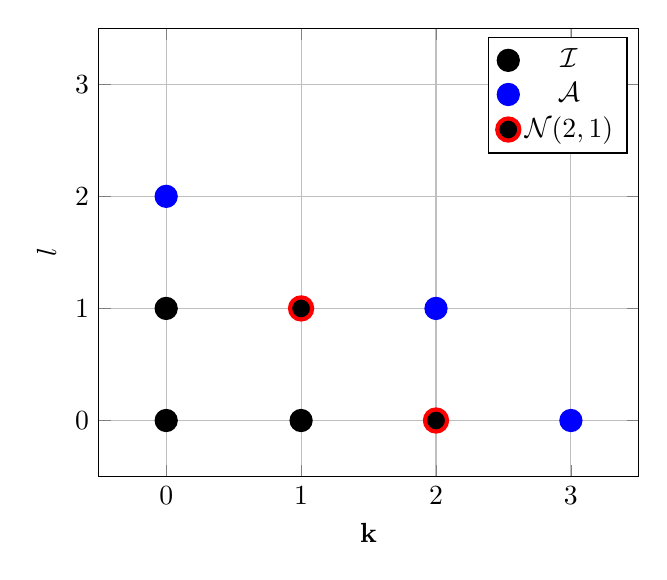
\begin{tikzpicture}

\begin{axis}[
xmin=-0.5, xmax=3.5,
ymin=-0.5, ymax=3.5,
axis on top,
xmajorgrids,
ymajorgrids,
xlabel=$\mi$,
ylabel=$l$
]
\addplot [only marks,mark size=4, draw=black, fill=black]
table {%
x                      y
+0.000000000000000e+00 +0.000000000000000e+00
+1.000000000000000e+00 +0.000000000000000e+00
+0.000000000000000e+00 +1.000000000000000e+00
+2.000000000000000e+00 +0.000000000000000e+00
+1.000000000000000e+00 +1.000000000000000e+00
};
\addplot [only marks, mark size=4,draw=blue, fill=blue]
table {%
x                      y
+3.000000000000000e+00 +0.000000000000000e+00
+2.000000000000000e+00 +1.000000000000000e+00
+0.000000000000000e+00 +2.000000000000000e+00
};
\addplot [only marks,mark size=4,line width=1.5, draw=red, fill=black]
table {%
x                      y
+1.000000000000000e+00 +1.000000000000000e+00
+2.000000000000000e+00 +0.000000000000000e+00
};
\addlegendentry{$\mis$};
\addlegendentry{$\mia$};
\addlegendentry{$\neighbors(2,1)$};
\end{axis}

\end{tikzpicture}
	\caption{Example with $d=1$ of a multi-index set $\mis$ and the associated set of admissible multi-indices $\mia$, as well as neighbors $\neighbors(2,1)$ of  $(2,1)\in\mia$. In this example $L=1$,  $\vsp_{1}=\vspan\{1,\psmi,\dots,\psmi^{6}\}=\vspan\{\leg_0(\psmi),\dots,\leg_{6}(\psmi)\}$, and  $\vsp_{0}=\vspan\{1,\psmi,\psmi^2\}=\vspan\{\leg_0(\psmi),\leg_1(\psmi),\leg_2(\psmi)\}$.}
	\label{fig:dc}
\end{figure}

We next explain how we arrive at the gain and work estimates that are required in step (i).
To estimate the norm of the orthogonal projection of $\rs_l-\rs_{l-1}$ onto $\pss_{\mi}$, we compute the arithmetic average of corresponding estimates for the neighbors $\neighbors(\mi,l)=\{(\mi^{(1)},l^{(1)}),\dots\}$ of $(\mi,l)$ in $\mathcal{I}$. Here, by neighbor we mean elements of $\mis$ that differ from $(\mi,l)$ in a single entry by $1$, see \Cref{fig:dc}.
For each such neighbor, we estimate the norm of the orthogonal projection $\operatorname{Proj}_{\mi^{(j)}}(\rs_{l^{(j)}}-\rs_{l^{(j)}-1})$ of $\rs_{l^{(j)}}-\rs_{l^{(j)}-1}$ onto $\pss_{\mi^{(j)}}$ simply by computing the Euclidean norm of those basis coefficients of $\P_{L-l^{(j)}}(\rs_{l^{(j)}}-\rs_{l^{(j)}-1})$ that belong to $\pss_{\mi^{(j)}}$. (Recall that $\P_{L-l^{(j)}}$ is a discrete projection onto the space $\vsp_{L-l^{(j)}}$ of which $\pss_{\mi^{(j)}}$ is a subspace since $\mi^{(j)}\in\mis_{l^{(j)}}$.)
The final estimate can be expressed as
\begin{equation*}
\frac{1}{|\neighbors(\mi,l)|}\sum_{j=1}^{|\neighbors(\mi,l)|}\norm{\operatorname{Proj}_{\mi^{(j)}}\P_{L-l^{(j)}}(\rs_{l^{(j)}}-\rs_{l^{(j)}-1})}{L^2_{\lambda}([0,1]^d)}.
\end{equation*}


To estimate the work that adding $(\mi,l)$ to $\mis$ incurs, we observe that \Cref{eq:adaptivestability} tells us exactly how many new samples are needed. More specifically, if we denote by $\NS(\mis_{l})$ the minimal solution of \Cref{eq:adaptivestability} for the polynomial subspace determined by $\mis_l$, then the required number of new samples of $\rs_{l}-\rs_{l-1}$ is $\NS(\mis_{l}\cup\{\mi\})-\NS(\mis_{l})$. It therefore remains to determine the  work per sample,  $\work(\rs_{l}-\rs_{l-1})$. If this work is unknown, then we store for each level $l$ an estimate, which we update with the observed computational work divided by the number of generated samples each time $\mathcal{I}_{l}$ changes. The final estimate of the work associated with $(\mi,l)$ is
\begin{equation*}
  \work(\rs_{l}-\rs_{l-1}) \cdot\left(\NS(\mis_{l}\cup\{\mi\})-\NS(\mis_{l})\right).
\end{equation*}

%\Cref{fig:dc} shows an example of $\mis$ and $\mia$ in the case $d=1$. In this case, the polynomial subspaces are simply spaces of polynomials with degree less than or equal to some natural number; more specifically, \Cref{fig:dc} represents the case
\Cref{alg:adaptive} gives a summary of our algorithm in pseudocode.
%\begin{rem}[Alternative multilevel construction]
%From the description of the multilevel method in terms of multi-indices as in \Cref{fig:dc}, one sees that one could alternatively first group all the indices that agree in the $\mi$ component instead of the $l$ component, which would yield approximations of the form
%$$
%\P_{\vsp_{0}}f_{L}+\sum_{l=1}^{L}\P_{\vsp_l\ominus \vsp_{l-1}}\rs_{L-l},
%$$
%where $\vsp_{l}\ominus\vsp_{l-1}$ denotes the orthogonal complement of $\vsp_{l-1}$ %in $\vsp_{l}$.
%\end{rem}


\begin{algorithm}[ht]
\caption{Adaptive multilevel algorithm.}\label{alg:adaptive}
\begin{algorithmic}[1]
		\Function{MLA}{$(\rs_l)_{l\in\N}$,STEPS}
		\State  $\mis\gets \{\mathbf{0}\}$
		\State $X_l\gets \varnothing\;\forall l\in\N$
		\State $\Delta_l\gets 0\;\forall l\in\N$
		\For{$0\leq i<\text{STEPS}$}
			\State $(\mi,l)\gets \argmax_{(\mi,l)\in\mia}\frac{\text{GAIN}((\mi,l),(\Delta_l)_{l\in\N},\mis)}{\text{WORK}((\mi,l),\mis)}$
			\State $N_{+}\gets \NS(\mis_{l}\cup\{\mathbf{k}\})-\NS(\mis_{l})$
			\State $\mis\gets \mathcal{I}\cup\{(\mi,l)\}$
			\For{$0\leq j<N_{+}$}
				\State Generate $\psmi\sim \arcsine_{d}$
				\State $y\gets (\rs_{l}-\rs_{l-1})(\psmi)$
				\State $X_l\gets X_l\cup\{(\psmi,y)\}$
			\EndFor
			\State $\Delta_l\gets \P_{L-l}(\rs_{l}-\rs_{l-1})$
		\EndFor
		\State \Return $\sum_{0\leq l\leq L}\Delta_l$
	\EndFunction
	\item[]
	\Function{GAIN}{$(\mi,l)$,$(\Delta_l)_{l\in\N}$,$\mathcal{I}$}
		\State $s=0$
		\For{$(\mi^{(j)},l^{(j)})\in \neighbors(\mi,l)$}
			\State $s\gets s+\|\operatorname{Proj}_{\mi^{(j)}}\Delta_{l^{(j)}} \|_{L^2_{\lambda}}$
		\EndFor

		\State \Return $s/|\neighbors(\mathbf{k},l)|$
	\EndFunction
	\item[]
	\Function{WORK}{$(\mi,l)$,$\mathcal{I}$}
		\State \Return $\work(\rs_{l}-\rs_{l-1})\cdot\left(\NS(\mis_{l}\cup\{\mi\})-\NS(\mis_{l})\right)$
	\EndFunction

\end{algorithmic}
\end{algorithm}

\section{Application to parametric PDE}
\label{sec:uq}
%In this section, we discuss the applicability of \Cref{thm:main,thm:main2} to problems in uncertainty quantification.

We assume in this section that $\pde(\cdot,\psmi)$ is the solution of some partial differential equation (PDE) with parameters $\psmi\in\domPS\subset\R^\dps$ and that we are interested in the \emph{response surface}
\begin{equation*}
\psmi\mapsto \rs_{\infty}(\psmi):=\QoI(\pde(\cdot,\psmi))\in\R,
\end{equation*}
where $\QoI(\pde(\cdot,\psmi))$ is a real-valued quantity of interest, such as a point evaluation, a spatial average, or a maximum.  
In most situations, we cannot evaluate $\rs_{\infty}(\psmi)$ exactly, as this would require an analytic solution of the PDE. Instead, we have to work with discretized solutions $\pde_{n}(\cdot,\psmi)$ for each $\psmi$, which yield approximate response surfaces
\begin{equation*}
\begin{split}
\rs_{n}\colon &\domPS\to\R \\
&\psmi\mapsto Q(\pde_{n}(\cdot,\psmi)).
\end{split}
\end{equation*}
For example, if we employ finite element discretizations with maximal element diameter $h:=n^{-1}$, then the work required for evaluations of $\rs_{n}$ grows like $h^{-\gamma}=n^{\gamma}$ for some $\gamma>0$. To apply the multilevel method of \Cref{sec:nonadaptive}, we need to verify the remaining Assumptions A1 and A2 from there. 

%consider parametric partial differential equations of the form
%\begin{equation}
%\label{eq:PDE}
%\begin{split}
%\PDE_y(u)=\rs_y
%\end{split}
%\end{equation}
%where both operator  $\PDE_y$ and right-hand side $\rs_y$ may depend on a %parameter $y\in\domPS\subset\mathbb{R}^d$ with $d\in\N\cup\{\infty\}$.%
% Assuming that there is a unique solution $u_y:=\PDE_y^{-1}(\rs_y)$ for each $y\in\domPS$, our goal is to approximate the dependence of a scalar, possibly nonlinear, quantity of interest $\qoi(u_y)$ on the parameter $y$.
As a motivating example, we consider a linear elliptic second order PDE, which has been extensively studied in recent years \cite{harbrecht2013multilevel,ChkifaCohenSchwab2015,CohenDevoreSchwab2011,BabuskaTemponeZouraris2004},
\begin{equation}
\label{eq:UQex}
\begin{aligned}
-\nabla \cdot (a(x,\psmi) \nabla \pde(x,\psmi))&=\rhs(x)&\text{ in }U\subset\R^{\dpde}\\
\pde(x,\psmi)&=0&\text{ on } \partial U,
\end{aligned}
\end{equation}
with $a:U\times \domPS\to\R$ and $\domPS:=[0,1]^\dps$. 


%If $\rhs\in H^{-1}(U)$ and
%\begin{equation}
%\inf_{x\in U}a(x,\psmi)>0\quad \forall \psmi\in\domPS,
%\end{equation}
%then the Lax-Milgram theorem guarantees existence of a unique solution $\pde(\cdot,\psmi)\in H_0^1(U)$ for all $\psmi\in\domPS$. In order to obtain convergence of 
\begin{pro}
	\label{pro:finite}
	For any $n\in\N$, let $\pde_{n}$ be finite element approximations of order $r\geq 1$ and maximal element diameter $h:=(n+1)^{-1}$, and let $\rs_{n}(\psmi):=Q(\pde_n(\cdot,\psmi))$.
	Assume that $g$ and $U$ are sufficiently smooth, that 
	\begin{equation}
		\inf_{x\in U,\psmi\in\domPS}a(x,\psmi)>0,
	\end{equation}
	and that $Q$ is a continuous linear functional on $L^2(U)$.
	
	
	
	\begin{enumerate}[(i)]
		\item If $a\in C^{r}(U\times\domPS)$ for some $r\geq 1$, then  %$\norm{\partial_{x}^{\mathbf{r}}\partial_{\psmi}^{\mathbf{s}}a}{C^0(U\times \domPS)}<\infty$ for all $|\mathbf{r}|_{1}+|\mathbf{s}|_{1}\leq r$, then 
		\begin{equation*}
		\norm{\rs_{\infty}-\rs_{n}}{L^2(\domPS)}\lesssim h^{r+1}
		\end{equation*}
		and
		\begin{equation*}
		\norm{\rs_{\infty}-\rs_{n}}{C^{r-1}(\domPS)}\lesssim h^{2}.
		\end{equation*}
		\item If for some $r,s\geq 1$ we have
		\begin{equation}
		\label{eq:tensor}
		\begin{split}
		a\in C^{r}(U)\otimes C^{s}(\domPS):=\{a\colon U\times \domPS\to\R :  \norm{\partial_{x}^{\mathbf{r}}\partial_{\psmi}^{\mathbf{s}}a}{C^0(U\times\domPS)}<\infty\;\forall\;|\mathbf{r}|_{1}\leq r,|\mathbf{s}|_{1}\leq s\}
		,
		\end{split}
		\end{equation} then 
		\begin{equation*}
		\norm{\rs_{\infty}-\rs_{n}}{C^{s}(\domPS)}\lesssim h^{r+1}.
		\end{equation*}
		
	%	\item If there exists $s\geq $ such that $\norm{\partial_{x}^{\mu}\partial_{\psmi}^{\nu}a}{C^0(U\times \domPS)}<\infty$ for all $|\mu|_{1}\leq r,|\nu|_{1}\leq s$ for some $s\geq 1$, then 
	%	\begin{equation*}
	%	\norm{\rs_{\infty}-\rs_{n}}{C^{s}_{\mix}(\domPS)}\lesssim h^{r+1}.
	%	\end{equation*}
	\end{enumerate}
\end{pro}
\begin{proof}
	In both cases, the standard theory of second order elliptic differential equations shows that $\psmi\mapsto \pde(\cdot,\psmi)$ is well defined as a map from $\domPS$ into $H^{r+1}(U)$, with 
	\begin{equation*}
	\norm{\pde}{L^\infty(\domPS;H^{r+1}(U))}<\infty.
	\end{equation*}
	Next, we observe that the derivatives $\partial_{\psmi_{j}}\pde(\cdot,\psmi)$, $j\in \{1,\dots,d\}$ satisfy PDEs with the same operator as in \Cref{eq:UQex} but with new right-hand sides
	\begin{equation*}
	\tilde{\rhs}(x):=\nabla\cdot(\partial_{\psmi_j}a(x,\psmi)\nabla \pde(x,\psmi)).
	\end{equation*}
	The regularity of this right-hand side now depends on the assumptions on the coefficient $a$.
	In case (i) we have $\partial_{\psmi_j}a(\cdot,\psmi)\in C^{r-1}(U)$ and thus $\tilde{\rhs}\in H^{r-2}(U)$. Therefore, $\partial_{\psmi_{j}}\pde(\cdot,\psmi)\in H^{r}(U)$ for each $\psmi\in\domPS$ and, moreover, we have the uniform estimate
		\begin{equation*}
		\norm{\partial_{\psmi_j}\pde}{L^\infty(\domPS;H^{r}(U))}<\infty.
		\end{equation*}
		In case (ii) we have $\partial_{\psmi_j}a(\cdot,\psmi)\in C^{r}(U)$ and thus $\tilde{\rhs}\in H^{r-1}(U)$. Therefore, $\partial_{\psmi_{j}}\pde(\cdot,\psmi)\in H^{r+1}(U)$ for each $\psmi\in\domPS$ and, moreover, we have the uniform estimate
		\begin{equation*}
		\norm{\partial_{\psmi_j}\pde}{L^\infty(\domPS;H^{r+1}(U))}<\infty.
		\end{equation*}
		Repeatedly applying these arguments yields
			\begin{equation*}
			\norm{\pde}{C^{r-1}(\domPS;H^2(U))}<\infty,
			\end{equation*}
			and
			\begin{equation*}
			\norm{\pde}{C^{s}(\domPS;H^{r+1}(U))}<\infty,
			\end{equation*}
%			or
%			\begin{equation*}
%			\norm{\pde}{C^{s}_{\mix}(\domPS;H^{r+1}(U))}<\infty,
%			\end{equation*}
		in cases (i) and (ii), respectively. We may now conclude by using standard finite-element theory. In case (i), we have
		\begin{equation*}
		\begin{split}
		\norm{\rs_{\infty}-\rs_{n}}{L^2(\domPS)}&\leq \norm{Q}{}\norm{\pde-\pde_{n}}{L^2(\domPS;L^2(U))}\\
		&\lesssim h^{r+1}\norm{\pde}{L^2(\domPS;H^{r+1}(U))}
		\end{split}
		\end{equation*}
		and
		\begin{equation*}
		\begin{split}
		\norm{\rs_{\infty}-\rs_{n}}{C^{r-1}(\domPS)}&\lesssim \norm{\pde-\pde_{n}}{C^{r-1}(\domPS;L^2(U))}\\
		&\lesssim h^{2}\norm{\pde}{C^{r-1}(\domPS;H^{2}(U))},
		\end{split}
		\end{equation*} 
	whereas in case (ii), we have
	\begin{equation*}
	\begin{split}
	\norm{\rs_{\infty}-\rs_{n}}{C^{s}(\domPS)}&\lesssim \norm{\pde-\pde_{n}}{C^{s}(\domPS;L^2(U))}\\
	&\lesssim h^{r+1}\norm{\pde}{C^{s}(\domPS;H^{r+1}(U))},
	\end{split}
	\end{equation*}
\end{proof}
\begin{rem}
In case (i) of the previous proposition, differentiating with respect to $\psmi$ reduces the number of available derivatives in $x$, which are required for convergence of the finite element method. Thus, the convergence in $L^2(\domPS)$ is faster than that in $C^{r-1}(\domPS)$. Case (ii), on the other hand, describes the so-called \emph{mixed smoothness} of the coefficient in $x$ and $\psmi$, meaning that differentiating in $\psmi$ does not affect the differentiability with respect to $x$.  
\end{rem}
 % Roughly speaking, it can be shown that for \Cref{eq:UQex} the response surface $\rs_{\infty}$ is as regular with respect to $\psmi$ as the diffusion coefficient $a_{\psmi}$. For example, if $a_{\psmi}$ is $s$ times differentiable with respect to $\psmi$ and the functional $\QoI$ is $s$ times differentiable with respect to $u$ (both in a suitable sense), then $\rs_{\infty}$ is $s$ times differentiable as well. % and lies in a Sobolev or a Hölder space of functions on $\domPS$ depending on the specifics of the problem and on the integrability of the derivatives $\partial^{s}_{\psmi}a_{\psmi}$. 
If the coefficients depend analytically on $\psmi$, then the same holds for $\rs_{\infty}$, which can be exploited to obtain algebraic polynomial approximability rates of $\rs_{\infty}$ even in the case of infinite-dimensional parameters \cite{ChkifaCohenSchwab2015,Haji-AliNobileTamelliniEtAl2015}, as shown below.

%However, to obtain strong convergence, we need not only know that $\rs_{\infty}\in \F$  for some space $\F$ with good polynomial approximability properties, but that 
%\begin{equation*}
%\norm{\rs_{\infty}-\rs_{n}}{\F}\lesssim n^{-\sc}
%\end{equation*}
%for some $\sc>0$. Estimates of this type have been established for example in \cite{harbrecht2013multilevel,Haji-AliNobileTamelliniEtAl2015}. An example of such an estimate is provided in \Cref{pro:UQ} below. 

%The underlying idea of this example is that the strong convergence rate $\sc=1$ can usually be obtained in any space $\F$ such that $\rs_{\infty}\in \F$. 

\begin{pro}
\label{pro:UQ}
Let $\domPS:=[-1,1]^{\infty}$.
Assume that $Q$ is a linear and continuous functional on $L^2(U)$, that $0<\inf_{x,\psmi}  a(x,\psmi)\leq \sup_{x,\psmi}  a(x,\psmi)<\infty$, and that
	\begin{align*}
	a(x,\psmi)&=\bar{a}(x)+\sum_{j=0}^{\infty}\ps_j\psi_j(x),\\
		a(x,\psmi)&=\bar{a}(x)+\left(\sum_{j=0}^{\infty}\ps_j\psi_j(x)\right)^2,\quad \\
	\intertext{or}
		a(x,\psmi)&=\exp\left(\sum_{j=0}^{\infty}\ps_j\psi_j(x)\right). 
	\end{align*}
	If there exists $r_{\max}>1$ such that
	\begin{equation*}
	 \|\psi_j\|_{C^{r}(U)}\lesssim (j+1)^{-(r_{\max}+1 - r)}\quad\forall j\in\N, \; 0\leq r< r_{\max},
	 \end{equation*} 
	 	 then, for any $r\in \N$ with $1\leq r< r_{\max}$, finite element approximations with maximal element diameter $h:=(n+1)^{-1}$ achieve
\begin{equation*}
\norm{\rs_{\infty}-\rs_{\n}}{L^{\infty}(\domPS)}\leq C h^{r+1}
\end{equation*}
with a constant $C$ independent of $n$.
Furthermore, for any such $r$, there is a sequence $(\vsp_\dvsp)_{\dvsp\in\N}$ of downward closed polynomial spaces with $\dim \vsp_\dvsp=m$ such that finite element approximations with order $r$ and maximal diameter $h:=(n+1)^{-1}$ achieve 
\begin{equation*}
e_{\vsp_\dvsp,1,\infty}(\rs_{\infty}-\rs_\n)\leq C(\dvsp+1)^{-\uqsummability}h^{r+1} \quad \forall\, 0<\uqsummability<r_{\max}- r
\end{equation*}
with a constant $C$ independent of $n$ and $m$.
%and
%\begin{equation*}
%e_{\vsp_\dvsp,2}(\rs_{\infty}-\rs_\n)\leq C(\dvsp+1)^{-\uqsummability}h^{r+1},\quad \forall \uqsummability<r_{\max}-\delta r-\frac{1}{2}
%\end{equation*}
\end{pro}
\begin{proof}
	
	It was shown in \cite[Theorem 4.1 \& Section 5]{ChkifaCohenSchwab2015} that for each $0\leq r<r_{\max}$ there exists a set $\domPS_{r}\subset \C^{\infty}$, $\domPS\subset \domPS_{r}$ such that
	$\norm{a}{L^{\infty}(\domPS_{r};C^{r}(U))}<\infty$ and such that $\psmi\mapsto \pde(\cdot,\psmi)$ may be extended to a complex differentiable map from $\domPS_{r}$ into $H^{1+r}(U)$ with
		\begin{equation}
		\label{eq:complexbounds}
		\begin{split}
	\norm{\pde}{L^{\infty}(\domPS_{r};H^{1+r}(U))}<\infty
		\end{split}
		\end{equation}
	
For a detailed description of the sets $\domPS_{r}$ we refer to \cite{ChkifaCohenSchwab2015}. For our purposes it suffices to know that the better the summability of $(\norm{\psi_j}{C^{r}(U)})_{j\in\N}$, the larger $\domPS_{r}$ can be chosen; and the larger $\domPS_{r}$ the better the polynomial approximability properties of complex differentiable maps defined on $\domPS_{r}$.
In particular, the results of \cite[Section 2]{ChkifaCohenSchwab2015}, show that when  restricted to the smaller set $\domPS$ such maps may be approximated at algebraic convergence rates within downward closed polynomial subspaces. More specifically, \cite[Equation (2.27)]{ChkifaCohenSchwab2015} shows that if a function $e$ is complex differentiable on $\domPS_{r}$, then for any $\dvsp\in\N$ there exists a downward closed polynomial subspace $\vsp_{\dvsp}$ such that
	\begin{equation*}
	\begin{split}
	\inf_{\tilde{\p}\in \vsp_{\dvsp}\otimes L^2(U)}\norm{e-\tilde{\p}}{L^\infty(\domPS;L^2(U))}\lesssim (\dvsp+1)^{-\alpha} \norm{e}{L^\infty(\domPS_{r};L^2(U))}
	\end{split}
	\end{equation*}
	for all $\alpha<r_{\max}- r$. 
 Applying this estimate with $e:=\pde-\pde_{n}$ shows
	\begin{equation*}
	\begin{split}
	\inf_{\p\in\vsp_{\dvsp}}\norm{(\rs_{\infty}-\rs_{\n})-\p}{L^\infty(\domPS)}&\leq \norm{Q}{} \inf_{\tilde{\p}\in \vsp_{\dvsp}\otimes L^2(U)}\norm{(\pde-\pde_n)-\tilde{\p}}{L^\infty(\domPS;L^2(U))}\\
\lesssim & (\dvsp+1)^{-\alpha} \norm{\pde-\pde_{n}}{L^\infty(\domPS_{r};L^2(U))}.
	\end{split}
	\end{equation*}

By standard finite element analysis we finally obtain
\begin{equation*}
\norm{\pde-\pde_{n}}{L^{\infty}(\domPS_{r};L^2(U))}\leq C h^{r+1}\norm{\pde}{L^{\infty}(\domPS_{r};H^{r+1}(U))}.
\end{equation*}
with  $C=C\big(	\norm{a}{L^{\infty}(\domPS_{r};C^{r}(U))}\big)<\infty$. Combining the previous two estimates with \Cref{eq:complexbounds} concludes the proof.
\end{proof}

\begin{rem}
	Similar results can also be shown for PDEs of parabolic type and for some nonlinear PDEs \cite{ChkifaCohenSchwab2015}.
\end{rem}
\section{Numerical implementation and solution}
In this section, we explain how to implement and solve the minimization problem \eqref{eq:dynamic_recon} numerically which, depending on the amount of time steps $T$, can be challenging. 
We derive a general primal-dual algorithm for its solution, before we line out some strategies to reduce computational costs and speed up the implementation at the end of this section. 

\subsection{Gradients and sampling operators}
\label{subsec:implementation of operators}

In order to use the discrete total variation already defined in Section \ref{subsubsec:TV}, we need a discrete gradient operator that maps an image $u \in \C^N$ to its gradient $\nabla u \in \C^{N \times 2}$. 
Following \cite{ChambollePock}, we implement the gradient by standard forward differences. Moreover, we  will use its discrete adjoint, the negative divergence $-\diverg$, defined by the identity $\langle \nabla u, w \rangle_{\C^{N \times 2}} = - \langle u, \diverg(w) \rangle_{\C^N}$.
The inner product on the gradient space $\C^{N\times 2}$ is defined in a straightforward way as 
\begin{align*}
	\langle v,w \rangle_{\C^{N \times 2}} = \Real(v_1^* w_1) + \Real(v_2^* w_2),
\end{align*}
%
for $v,w \in \C^{N \times 2}$.
For $v \in \C^{N \times 2}$, the (isotropic) 1-norm is defined by 
\begin{align*}
	\|v \|_1 := \sum_{i=1}^N \sqrt{|(v_i)_1|^2 + |(v_i)_2|^2},
\end{align*}
and accordingly the dual $\infty$-norm for $w \in \C^{N \times 2}$ is given by 
\begin{align*}
	\| w \|_\infty := \max_{i=1,\cdots,N} |w_i| = \max_{i=1,\cdots,N} ~ \sqrt{|(w_i)_1|^2 + |(w_i)_2|^2}.
\end{align*}

The sampling operators $\Kcal_t \colon \C^N \to \C^{M_t}$ (and analogously for $\Kcal_0 \colon \C^{N_0} \to \C^{M_0}$) we consider are either a standard fast Fourier transform (FFT) on a Cartesian grid, followed by a projection onto the sampled frequencies, or a non-uniform fast Fourier transform (NUFFT), in case the sampled frequencies are not located on a Cartesian grid \cite{Fessler:NUFFT}. \\

\noindent {\it Fourier transform on a Cartesian grid - the simulated data case}\\
\noindent
In the numerical study on artificial data we use a simple version of the Fourier transform and sampling operator (the same can also be found in e.g. \cite{Ehrhardt2016,Rasch2017}). 
We discretize the image domain on the unit square using an (equi-spaced) Cartesian grid with $N_1 \times N_2$ pixels such that the discrete grid points are given by 
\begin{align*}
 \Omega_N = \left\{ \left(\frac{n_1}{N_1-1}, \frac{n_2}{N_2-1} \right) ~\Big|~ n_1 = 0, \dots, N_1-1, \; n_2 = 0, \dots N_2-1 \right\}.
\end{align*}
We proceed analogously with the $k$-space, i.e. the location of the $(m_1,m_2)$-th Fourier coefficient is given by $(m_1/(N_1-1), m_2/(N_2-1))$. Then, we arrive at the following formula for the (standard) Fourier transform $\Fcal$ applied to $u \in \C^{N_1 \times N_2}$:
\begin{align*}
 (\Fcal u)_{m_1,m_2} = \frac{1}{N_1 N_2} \sum_{n_1=0}^{N_1-1} \sum_{n_2=0}^{N_2-1} u_{n_1,n_2} e^{-2\pi i \left(\frac{n_1 m_1}{N_1} + \frac{n_2 m_2}{N_2} \right)},
\end{align*}
where $ m_1 = 0, \dots, N_1-1, m_2 = 0, \dots, N_2 -1$.
For simplicity, we use a vectorized version such that $\Fcal \colon \C^N \to \C^N$ with $N = N_1 \cdot N_2$.
We then employ a simple sampling operator $\Scal_t \colon \C^N \to \C^{M_t}$ which discards all Fourier frequencies which are not located on the desired sampling geometry at time $t$ (i.e. the chosen spokes). 
More precisely, following \cite{Ehrhardt2016}, if we let $\Pcal_t \colon \{1,\dots,M_t \} \to \{1,\dots,N\}$ be an injective mapping which chooses $M_t$ Fourier coefficients from the $N$ coefficients available, we can define the sampling operator $\Scal$ applied to $f \in \C^N$ as
\begin{align*}
 \Scal_t \colon \C^N \to \C^{M_t}, \quad (\Scal_t f)_k = f_{\Pcal_t(k)}.
\end{align*}
The full forward operator $\Kcal_t$ can hence be expressed as 
\begin{align}\label{eq:forward_op_art}
 \Kcal_t \colon \C^N \xrightarrow{\Fcal} \C^N \xrightarrow{\Scal_t} \C^{M_t}.
\end{align}
The corresponding adjoint operator of $\Kcal_t$ is given by  
\begin{align*}
 \Kcal_t^* \colon \C^{M_t} \xrightarrow{\Scal_t^*} \C^N \xrightarrow{\Fcal^{-1}} \C^N,
\end{align*}
where $\Fcal^{-1}$ denotes the standard inverse Fourier transform and $\Scal_t^*$ `fills' the missing frequencies with zeros, i.e. 
\begin{align*}
 (\Scal_t^*z)_l = \sum_{k=1}^{M_t} z_k \delta_{l,\Pcal_t(k)}, \qquad \text{for } l = 1, \dots, N.
\end{align*}
For the prior $u_0$, we choose a full Cartesian sampling, which corresponds to $\Pcal_0$ being the identity. For the subsequent dynamic scan, we set up $\Pcal_t$ such that it chooses the frequencies located on (discrete) spokes through the center of the $k$-space.     
It is important to notice that this implies that the locations of the (discretized) spokes are still located on a Cartesian grid, which allows to employ a standard fast Fourier transform (FFT) followed by the above projection onto the desired frequencies. 
This is not the case for the operators we use for real data. \\

\noindent {\it Non-uniform Fourier transform - the real data case}\\ 
\noindent 
In contrast to the above (simplified) setup for artificial data, in many real world application the measured $k$-space frequencies $\xi_m$ in \eqref{eq:fourier_transform} are {\it not} located on a Cartesian grid. 
While this is not a problem with respect to the formula itself, it however excludes the possibility to employ a fast Fourier transform, 
%numerically
which usually reduces the computational costs of an $N$-point Fourier transform from an order of $O(N^2)$ to $O(N \log N)$.
To get to a similar order of convergence also for non-Cartesian samplings, it is necessary to employ the concept of non-uniform fast Fourier transforms (NUFFT) \cite{Fessler:NUFFT,Fessler:code,Matej2004,Nguyen:1999,Strohmer2000}. 
We only give a quick intuition here and for further information we refer the reader to the literature listed above. 
The main idea is to use a (weighted) and oversampled standard Cartesian $K$-point FFT $\Fcal$, $K \geq N$ followed by an interpolation $\Scal$ in $k$-space onto the desired frequencies $\xi_m$. 
Note that the oversampling takes place in $k$-space.
The operator $\Kcal_t$ for time $t$ can hence again be expressed as a concatenation of a $K$-point FFT and a sampling operator 
\textbf{\begin{align*}
 \Kcal_t \colon \C^N \xrightarrow{\Fcal} \C^N \xrightarrow{\Scal_t} \C^{M_t}.
\end{align*}}
For our numerical experiments with the experimental DCE-MRI data, the sampling operator $\Scal_t$ and its adjoint were taken from the NUFFT package \cite{Fessler:code}.

\subsection{Numerical solution}
%
Due to the nondifferentiablity and the involved operators we apply a primal-dual method \cite{ChambollePock} to solve the minimization problem \eqref{eq:dynamic_recon}. 
We first line out how to solve the (simple) TV-regularized problem for the prior (\ref{tvu0}) and then extend the approach to the dynamic problem. 
Interestingly, the problem for the prior already provides all the ingredients needed for the numerical solution of the dynamic problem, which can then be done in a very straightforward way. 
We consider the problem 
\begin{equation} \label{tvu0}
	\min_{u_0} ~ \frac{\alpha_0}{2} \| \Kcal_0 u_0 - f_0 \|_{\C^{M_0}}^2 + \| \nabla u_0 \|_1, 
\end{equation}
with $u_0 \in \C^{N_0}$.
Dualizing both terms leads to its primal-dual formulation 
\begin{align}\label{eq:tv_pd}
	\min_{u_0} \max_{y_1,y_2} ~ \langle y_1, \Kcal_0 u_0 - f_0 \rangle_{C^{M_0}} - \frac{1}{2 \alpha_0} \|y_1 \|_{\C^{M_0}}^2 + \langle y_2, \nabla u_0 \rangle_{\C^{N_0 \times 2}} + \chi_{C}(y_2),
\end{align}
where $y_1 \in \C^{M_0}$ and $\chi_{C}$ denotes the characteristic function of the set  
\begin{align*}
	C := \{ y \in \C^{N_0 \times 2} ~|~ \|y \|_\infty \leq 1 \}.
\end{align*}
% 
The primal-dual algorithm in \cite{ChambollePock} now essentially consists in performing a proximal gradient descent on the primal variable $u_0$ and a proximal gradient ascent on the dual variables $y_1$ and $y_2$, where the gradients are taken with respect to the linear part, the proximum with respect to the nonlinear part. 
We hence need to compute the proximal operators for the nonlinear parts in \eqref{eq:tv_pd} to obtain the update steps for $u_0$ and $y_1,y_2$. 
It is easy to see that the proximal operator for $\phi(y_1) = \frac{1}{2 \alpha} \|y_1\|_{\C^{M_0}}^2$ is given by 
\begin{align}\label{eq:prox_dual_l2}
	y_1 = \prox_{\sigma \phi} (r) \Leftrightarrow y_1 = \frac{\alpha r}{\alpha + \sigma}.
\end{align}
The proximal operators for the update of $y_2$ are given by a simple projection onto the set $C$, i.e. 
\begin{align}\label{eq:prox_proj}
	y_2 = \proj_C (r) \Leftrightarrow (y_2)_i = r_i / \max (|r_i|,1) \quad \text{for all } i.
\end{align}
Putting everything together leads to Algorithm \ref{alg:prior}.
\begin{algorithm}[t!] 
\caption{\textbf{Reconstruction of the prior}}
{
\begin{algorithmic}[1]
\Require step sizes $\tau,\sigma > 0$, data $f_0$, parameter $\alpha_0$
\Ensure $u_0^0 = \bar{u}_0^0 = \Kcal_0^*f_0, ~ y_1^0 = y_2^0 = 0$
	\While{$\sim$ stop crit}
    	\State {\it Dual updates}
        \State $y_1^{k+1} = (\alpha_0 \left[ y_1^k + \sigma (\Kcal_0 \bar{u}_0^k - f_0)\right]) / (\alpha_0 + \sigma)$
          \State $y_2^{k+1} = \proj_C \left(y_2^k + \sigma \nabla \bar{u}_0^k\right)$
          \State {\it Primal updates}
          \State $u_0^{k+1} =  u_0^k - \tau \left[ \Kcal_0^* y_1^{k+1} - \diverg(y_2^{k+1}) \right]$
          \State {\it Overrelaxation}
          \State $\bar{u}_0^{k+1}= 2 u_0^{k+1} - u_0^k$
	\EndWhile\\
\Return $u_0 = u_0^k$
\end{algorithmic}
}
\label{alg:prior}
\end{algorithm}
\ \\

The numerical realization of the dynamic problem is now straightforward.
In order to deal with the infimal convolution, we use its definition and introduce an additional auxiliary variable yielding 
\begin{alignat*}{4}
	&\min_{\ubold}&& ~ &&\sum_{t=1}^T \frac{\alpha_t}{2} \| \Kcal_t u_t - f_t \|_{\C^{M_t}}^2 + \sum_{t=1}^{T-1} \frac{\gamma_t}{2} \|u_{t+1} - u_t \|_{\C_N}^2 + \sum_{t=1}^T w_t \TV(u_t) \\
	& && + && \sum_{t=1}^T (1-w_t) \ICBTV^{p_0}(u_t,u_0) \\    
   = &\min_{\ubold,\zbold}&& ~ &&\sum_{t=1}^T \frac{\alpha_t}{2} \| \Kcal_t u_t - f_t \|_{\C^{M_t}}^2 + \sum_{t=1}^{T-1} \frac{\gamma_t}{2} \|u_{t+1} - u_t \|_{\C_N}^2 +\sum_{t=1}^T w_t \| \nabla u_t \|_1\\
   & && + &&\sum_{t=1}^T (1-w_t) \left[ \| \nabla (u_t - z_t) \|_1 + \| \nabla z_t \|_1  - \langle p_0,u_t \rangle_{\C^N} + \langle 2 p_0, z_t \rangle_{\C^N} \right]
\end{alignat*}
where $\ubold = [u_1, \dots, u_T] \in \C^{N \times T}$ and $\zbold = [z_1, \dots, z_T] \in \C^{N \times T}$.
Introducing a dual variable $\ybold$ for all the terms containing an operator, leads to the primal-dual formulation 
\begin{alignat}{4}
\label{eq:primal_dual}
	&\min_{\ubold,\zbold} \max_{\ybold} && ~ && \sum_{t=1}^T \left(\langle y_{t,1}, \Kcal_t u_t - f_t \rangle_{\C^{M_t}} - \frac{1}{2 \alpha_t} \|y_{t,1} \|_{\C^M}^2 \right) + \sum_{t=1}^{T-1} \frac{\gamma_t}{2} \| u_{t+1} - u_t \|_{\C^N}^2 \notag \\
    & && + && \sum_{t=1}^T \left(\langle y_{t,2}, \nabla u_t \rangle_{\C^{N \times 2}} + \langle y_{t,3}, \nabla (u_t - z_t) _{\C^{N \times 2}} + \langle y_{t,4}, \nabla z_t \rangle_{\C^{N \times 2}}\right) \notag \\
    & && - && \sum_{t=1}^T \langle (1-w_t)p_0,u_t \rangle_{\C^N} + \sum_{t=1}^T \langle 2(1-w_t)p_0,z_t \rangle_{\C^N}  \notag \\
    & && + && \sum_{t=1}^T \left(\chi_{C_{t,2}}(y_{t,2}) + \chi_{C_{t,3}}(y_{t,3}) + \chi_{C_{t,4}}(y_{t,4})\right)
\end{alignat}
where $\ybold = [\ybold_1, \dots, \ybold_T]$, $\ybold_t = [y_{t,1}, \dots, y_{t,4}]$, and for all $t = 1, \dots, T$, $u_{t} \in \C^{M_t}$ and
\begin{align*}
	&C_{t,2} := \{ y \in \C^{M \times 2} ~|~ \|y \|_{\infty} \leq w_t \}, \\
    &C_{t,3} := \{ y \in \C^{M \times 2} ~|~ \|y \|_{\infty} \leq (1-w_t) \}, \\
    &C_{t,4} := \{ y \in \C^{M \times 2} ~|~ \|y \|_{\infty} \leq (1-w_t) \}. \\
\end{align*}
%
\begin{algorithm}[t!]
\caption{\textbf{Dynamic reconstruction with structural prior}}
{
\begin{algorithmic}[1]
\Require step sizes $\tau,\sigma > 0$, subgradient $p_0$, for all $t=1,\dots,T$: data $f_t$, parameters $\alpha_t$, $w_t$, $\gamma_t$
\Ensure for all $t=1,\dots,T$: $u_t^0 = \bar{u}_t^0 = \Kcal_t^*f_t, ~ z_t^0 = \bar{z}_t^0 = 0, ~ y_{t,1}^0 = y_{t,2}^0 = y_{t,3}^0 = y_{t,4}^0 = 0$
	\While{$\sim$ stop crit}
    	\For{t=1,\dots,T} 
          \State {\it Dual updates}
          \State $y_{t,1}^{k+1} = \frac{\alpha_t \left[ y_{t,1} + \sigma (\Kcal_t \bar{u}_t^k - f_t)\right]}{\alpha_t + \sigma}$
          \State $y_{t,2}^{k+1} = \proj_{C_2}\left(y_{t,2}^k + \sigma \nabla \bar{u}_t^k\right)$
          \State $y_{t,3}^{k+1} = \proj_{C_3}\left(y_{t,3}^k + \sigma \nabla (\bar{u}_t^k - \bar{z}_t^k) \right)$
          \State $y_{t,4}^{k+1} = \proj_{C_4}\left(y_{t,4}^k + \sigma \nabla \bar{z}_t^k \right)$
          \State {\it Primal updates}
          \State $u_t^{k+1} =  \frac{u_t^k - \tau \left[ \Kcal_t^* y_{t,1}^{k+1} - \diverg(y_{t,2}^{k+1}) - \diverg(y_{t,3}^{k+1}) - (1-w_t)p_0 \right] + \tau \gamma_t u_{t+1}^k + \tau \gamma_{t-1} u_{t-1}^k}{\tau (\gamma_t + \gamma_{t+1}) +1}$
          \State $z_t^{k+1} - \tau \left[ 2(1-w_t) p_0 + \diverg(y_{t,3}^{k+1}) - \diverg(y_{t,4}^{k+1}) \right]$
          \State {\it Overrelaxation}
          \State $(\bar{u}_t^{k+1}, \bar{z}_t^{k+1}) = 2 (u_t^{k+1}, z_t^{k+1}) - (u_t^k,z_t^k)$
    	\EndFor
	\EndWhile\\
\Return for all $t = 1,\dots,T$: $u_t = u_t^k$
\end{algorithmic}
}
\label{alg:fmri}
\end{algorithm}
%
To solve the problem, we again perform a proximal gradient descent on the primal variables $\ubold$ and $\zbold$, and a proximal gradient ascent on the dual variables $\ybold$, where the gradients are taken with respect to the linear parts, the proximum with respect to the nonlinear parts. 
We hence need to compute the proximal operators for the nonlinear parts in \eqref{eq:primal_dual} to obtain the update steps for $u_t,z_t$ and $\ybold_t$ for every $t = 1, \dots, T$. 
The proximal operators for $\phi_t(y_{t,1}) = \frac{1}{2 \alpha_t} \| y_{t,1} \|_{\C^{M_t}}^2$ can be computed exactly as in \eqref{eq:prox_dual_l2}.
The proximal operators for the updates of $y_{t,j}$, $j = 2,3,4$, are given by projections onto the sets $C_{t,j}$ similar to \eqref{eq:prox_proj}.
For the squared norm related to the time regularization, we notice that for every $1< t < T$, $u_t$ only interacts with the previous and the following time step, i.e. $u_{t-1}$ and  $u_{t+1}$. 
Hence, analogously to $\phi_t$, the proximum for 
\begin{align*}
	\psi_t(u_t) = \frac{\gamma_{t-1}}{2} \|u_t - u_{t-1}\|_{\C^N}^2 + \frac{\gamma_t}{2} \|u_{t+1} - u_t\|_{\C^N}^2
\end{align*}
is given by 
\begin{align*}
	u_t = \prox_{\tau \psi_t} (r) \Leftrightarrow u_t = \frac{r + \tau \gamma_t u_{t+1} + \tau \gamma_{t-1} u_{t-1}}{\tau (\gamma_t + \gamma_{t-1}) + 1}. 
\end{align*}
The two odd updates for $t = 1$ and $t = T$ can be obtained by the same formula by simply setting $\gamma_0 = 0$ and $\gamma_T = 0$, respectively.
Putting everything together, we obtain Algorithm \ref{alg:fmri}.\\

\subsection{Step sizes and stopping criteria}
We quickly discuss the choice of the step sizes $\tau, \sigma$ and stopping criteria for Algorithm \ref{alg:fmri}. 
In most standard applications it stands to reason to choose the step sizes according to the condition $\tau \sigma \| L \|^2 < 1$ ($L$ denotes the collection of all operators) such that convergence of the algorithm is guaranteed \cite{ChambollePock}.
However, depending on $T$, i.e. the number of time frames we consider, the norm of the operator $L$ 
can be very costly to compute, or too large such that the condition $\tau \sigma \| L \|^2 < 1$ only permits extremely small step sizes. 
For practical use, we instead simply choose $\tau$ and $\sigma$ reasonably ''small`` and track both the energy of the problem and the primal-dual residual \cite{Goldstein:Adaptive} to monitor convergence. 
For the sake of brevity, we do not write down the primal-dual residual for Algorithm \ref{alg:fmri} and instead refer the reader to \cite{Goldstein:Adaptive} for its definition. 
The implementation is then straightforward.
We hence stop the algorithm if both, the relative change in energy between consecutive iterates and the primal-dual residual, have dropped below a certain threshold.

\subsection{Practical considerations}
It is clear that for a large number of time frames $T$ Algorithm \ref{alg:fmri} starts to require an increasing amount of time to return reliable results and for reasonably ''large`` step sizes $\tau$ and $\sigma$ it is even doubtful whether we can obtain convergence. 
In practice, it is hence necessary to divide the time series $\Tbold = \{1, \dots, T\}$ into $l$ smaller bits of consecutive time frames. More precisely, choose numbers $1 \leq T_1 < \dots < T_l = T$ such that $\Tbold = \Tbold_1 \cup \Tbold_2 \cup \dots \cup \Tbold_l$ with $\Tbold = \{1, \dots, T_1, T_1+1, \dots, T_2, \dots, T_{l-1}+1, \dots, T_l\}$.
We can then perform the reconstruction separately for all $\Tbold_i$. 
In order to keep the ''continuity`` between $\Tbold_i$ and $\Tbold_{i+1}$, we can include the last frame of $\Tbold_i$ into the reconstruction of $\Tbold_{i+1}$ by letting $\gamma_{T_i} \neq 0$ and choosing $u_{T_i}$ as the respective last frame of $\Tbold_i$.
This divides the overall problem into smaller and easier subproblems, which can be solved faster.
In practice, we observed that a size of five to ten frames per subset $\Tbold_i$ is a reasonable choice, which essentially gives very similar results as doing a reconstruction for the entire time series $\Tbold$.







% \vspace{-0.5em}
\section{Conclusion}
% \vspace{-0.5em}
Recent advances in multimodal single-cell technology have enabled the simultaneous profiling of the transcriptome alongside other cellular modalities, leading to an increase in the availability of multimodal single-cell data. In this paper, we present \method{}, a multimodal transformer model for single-cell surface protein abundance from gene expression measurements. We combined the data with prior biological interaction knowledge from the STRING database into a richly connected heterogeneous graph and leveraged the transformer architectures to learn an accurate mapping between gene expression and surface protein abundance. Remarkably, \method{} achieves superior and more stable performance than other baselines on both 2021 and 2022 NeurIPS single-cell datasets.

\noindent\textbf{Future Work.}
% Our work is an extension of the model we implemented in the NeurIPS 2022 competition. 
Our framework of multimodal transformers with the cross-modality heterogeneous graph goes far beyond the specific downstream task of modality prediction, and there are lots of potentials to be further explored. Our graph contains three types of nodes. While the cell embeddings are used for predictions, the remaining protein embeddings and gene embeddings may be further interpreted for other tasks. The similarities between proteins may show data-specific protein-protein relationships, while the attention matrix of the gene transformer may help to identify marker genes of each cell type. Additionally, we may achieve gene interaction prediction using the attention mechanism.
% under adequate regulations. 
% We expect \method{} to be capable of much more than just modality prediction. Note that currently, we fuse information from different transformers with message-passing GNNs. 
To extend more on transformers, a potential next step is implementing cross-attention cross-modalities. Ideally, all three types of nodes, namely genes, proteins, and cells, would be jointly modeled using a large transformer that includes specific regulations for each modality. 

% insight of protein and gene embedding (diff task)

% all in one transformer

% \noindent\textbf{Limitations and future work}
% Despite the noticeable performance improvement by utilizing transformers with the cross-modality heterogeneous graph, there are still bottlenecks in the current settings. To begin with, we noticed that the performance variations of all methods are consistently higher in the ``CITE'' dataset compared to the ``GEX2ADT'' dataset. We hypothesized that the increased variability in ``CITE'' was due to both less number of training samples (43k vs. 66k cells) and a significantly more number of testing samples used (28k vs. 1k cells). One straightforward solution to alleviate the high variation issue is to include more training samples, which is not always possible given the training data availability. Nevertheless, publicly available single-cell datasets have been accumulated over the past decades and are still being collected on an ever-increasing scale. Taking advantage of these large-scale atlases is the key to a more stable and well-performing model, as some of the intra-cell variations could be common across different datasets. For example, reference-based methods are commonly used to identify the cell identity of a single cell, or cell-type compositions of a mixture of cells. (other examples for pretrained, e.g., scbert)


%\noindent\textbf{Future work.}
% Our work is an extension of the model we implemented in the NeurIPS 2022 competition. Now our framework of multimodal transformers with the cross-modality heterogeneous graph goes far beyond the specific downstream task of modality prediction, and there are lots of potentials to be further explored. Our graph contains three types of nodes. while the cell embeddings are used for predictions, the remaining protein embeddings and gene embeddings may be further interpreted for other tasks. The similarities between proteins may show data-specific protein-protein relationships, while the attention matrix of the gene transformer may help to identify marker genes of each cell type. Additionally, we may achieve gene interaction prediction using the attention mechanism under adequate regulations. We expect \method{} to be capable of much more than just modality prediction. Note that currently, we fuse information from different transformers with message-passing GNNs. To extend more on transformers, a potential next step is implementing cross-attention cross-modalities. Ideally, all three types of nodes, namely genes, proteins, and cells, would be jointly modeled using a large transformer that includes specific regulations for each modality. The self-attention within each modality would reconstruct the prior interaction network, while the cross-attention between modalities would be supervised by the data observations. Then, The attention matrix will provide insights into all the internal interactions and cross-relationships. With the linearized transformer, this idea would be both practical and versatile.

% \begin{acks}
% This research is supported by the National Science Foundation (NSF) and Johnson \& Johnson.
% \end{acks}
\paragraph{Acknowledgements} F. Nobile received support from the Center for ADvanced MOdeling Science (CADMOS). R. Tempone and S. Wolfers are members of the KAUST SRI Center for Uncertainty Quantification in Computational Science and Engineering. R. Tempone received support from the KAUST CRG3 Award Ref:2281 and the KAUST CRG4 Award Ref:2584.



%\clearpage
%\listoffigures
%\addcontentsline{toc}{section}{\refname}\printbibliography

\bibliography{library.bib}{}
\bibliographystyle{plain}
\end{document}
